\documentclass[a4paper, 12pt]{report}
\usepackage[italian]{babel}
%\usepackage[english]{babel}
\usepackage[a4paper, top=2cm, bottom=2cm, inner=2cm, outer=2cm, headheight=1cm, headsep=1cm, footskip=1cm]{geometry}
\usepackage{setspace} % Interlinea
%\usepackage{mathptmx} % Times New Roman
\usepackage[utf8]{inputenc}
\usepackage{graphicx, wrapfig} % Per il logo dell'università
\usepackage{amsmath}
\usepackage{float}
\usepackage{multicol}
\usepackage[hidelinks]{hyperref}
\usepackage{listings}
\usepackage[dvipsnames]{xcolor}
\usepackage{hyperref} % Gestisce gli URL e i collegamenti ipertestuali
\usepackage{breakurl} % Permette di spezzare gli URL lunghi
%\usepackage{minted}

% Pacchetto per le note a piè di pagina
\usepackage{footmisc}
\renewcommand{\footnotesize}{\fontsize{10pt}{10pt}\selectfont} % Note in 10 pt con interlinea singola

%latexmk -pdf -shell-escape tuo_documento.tex
\setlength{\parindent}{0pt}
\usepackage{amsmath,amssymb}

%\onehalfspacing

% Definizione del colore di sfondo e altre impostazioni
\definecolor{bggray}{rgb}{0.95, 0.95, 0.95}
\definecolor{keywords}{rgb}{0.0, 0.0, 0.6}
\definecolor{comments}{rgb}{0.0, 0.5, 0.0}
\definecolor{strings}{rgb}{0.6, 0.1, 0.1}

\lstset{
    language=Python,
    basicstyle=\ttfamily\small,
    backgroundcolor=\color{bggray},
    keywordstyle=\color{keywords}\bfseries,
    commentstyle=\color{comments}\itshape,
    stringstyle=\color{strings},
    frame=single,
    rulecolor=\color{black},
    numbers=left,
    numberstyle=\tiny,
    stepnumber=1,
    showstringspaces=false,
    tabsize=4,
    breaklines=true,
    breakatwhitespace=true
}

\begin{document}

    %%==========[RIASSUNTO]==========%%
    %\section*{Riassunto del contenuto della Tesi}
%\subsection*{Campo applicativo}
La tesi tratta l'applicazione delle reti neurali % al telerilevamento 
% , nello specifico di reti 
% convoluzionali (CNN), 
% Il telerilevamento, è una scienza che permette di identificare, misurare ed
% analizzare le caratteristiche qualitative e quantitative di una 
% determinata area di interesse senza entrare in contatto diretto con 
% essa. Tipicamente, l’oggetto di studio nel telerilevamento è il 
% pianeta Terra in tutte le sue componenti: territorio, acqua e atmosfera.
% Nello specifico, l'applicazione 
% delle reti neurali convoluzionali (CNN) all'agricoltura di precisione, 
per svolgere  
una mappatura delle colture agricole (\textit{Crop mapping}) 
utilizzando immagini satellitari Sentinel-2.
La mappatura delle colture è una delle molte applicazioni del telerilevamento e 
consiste nell’identificazione e classificazione delle colture agricole 
all'interno di un'area geografica.
Questa applicazione è fondamentale per supportare il 
processo decisionale e fornire inventari accurati e tempestivi per stimare la 
produzione e monitorare la crescita dinamica delle colture a varie scale. 
%\subsection*{Parte sperimentale}
La tesi è strutturata su otto capitoli:
Il primo capitolo tratta la definizione di rete neurale, di \textit{Deep learning} e di 
\text{Machine Learning}.
Viene inoltre illustrato il concetto di dataset ed i metodi che si utilizzano per 
valutare le prestazioni di un modello di \textit{Deep learning}.
Nel secondo capitolo vengono presentati i framework che permettono lo sviluppo di modelli 
di \textit{Deep learning}, il linguaggio di programmazione utilizzato per la realizzazione dei 
modelli ed il concetto di Tensore.
Nel terzo capitolo vengono richiamati i concetti fondamentali del
telerilevamento, illustrando come avviene l'acquisizione delle informazioni nel telerilevamento.
Nel quarto capitolo si approfondisce il funzionamento di una rete neurale classica, 
partendo dalle basi fino a trattare concetti più complessi.
Nel quinto capitolo vengono trattate le reti neurali convolutive, illustrando i principi 
su cui si basano queste tipologie di reti e gli elementi di cui sono composte. 
% Nel sesto capitolo vengono richiamati i concetti di base dietro alla segmentazione delle immagini.
% Sempre nello stesso capitolo, viene anche illustrata l'architettura UNet.
Nel sesto capitolo vengono trattati i concetti di base relativi alla segmentazione 
delle immagini. Illustrando anche l'architettura UNet, spesso utilizzata per applicazioni 
di segmentazione semantica delle immagini.
Il settimo capitolo tratta la sperimentazione, illustrando il processo per la realizzazione di 
un modello in grado di eseguire la segmentazione semantica su delle immagini satellitari.
% Mentre nell'ottavo capitolo vengono discussi i risultati ottenuti, mettendoli a confronto con i 
% risultati ottenuti da altri modelli applicati allo stesso problema. 
Nell'ottavo capitolo vengono discussi i risultati ottenuti, confrontandoli
con quelli ottenuti da altri modelli descritti in articoli che utilizzano lo stesso dataset.
Nella parte sperimentale della tesi è stato esposto l'intero 
procedimento per realizzare un sistema capace di apprendere 
automaticamente le caratteristiche di ogni campo agricolo, descrivendo i vari problemi riscontrati 
e le soluzioni adottate.
Per l'addestramento di questo sistema è stato utilizzo il dataset Sentinel2-Munich480, 
un dataset contenente immagini satellitari Sentinel-2 sull'area a nord di Monaco, in Germania.
Per lo sviluppo del modello sono state applicate due diverse architetture di reti neurali per la 
segmentazione semantica di immagini.
La prima versione del sistema era 
basata sull'architettura U-Net, ma presentava alcune limitazioni nel riconoscimento di molte colture agricole.
La seconda versione del sistema si basava invece su una versione dell'architettura U-Net che 
sfruttava le convoluzioni 3D. 
L'utilizzo di quest'ultima architettura, ha permesso al sistema di raggiungere un precisione 
del 91.92\% sul dataset di valutazione ed una precisione del 91.84\% sul dataset 
di validazione, raggiungendo risultati molto vicini allo stato dell'arte nel campo del 
crop mapping sul dataset Sentinel2-Munich480.






% \subsection*{Struttura della tesi}
% Il libro si articola in un'esauriente trattazione tecnica che 
% spazia dai fondamenti teorici dell'intelligenza artificiale (AI) e 
% dell'apprendimento automatico (Machine Learning, ML) fino a 
% specifiche applicazioni nel telerilevamento per la segmentazione 
% delle immagini, con particolare attenzione ai dati 
% satellitari Sentinel-2.

% Introduzione all'Intelligenza Artificiale, Machine Learning e Deep Learning
% Il primo capitolo introduce i concetti fondamentali di intelligenza artificiale, delineando l'evoluzione storica e i principi alla base di questa disciplina. Successivamente, il focus si sposta sul machine learning, descrivendone le definizioni, le modalità di apprendimento (supervisionato, non supervisionato e per rinforzo) e le principali categorie di problemi affrontati. La sezione dedicata al deep learning esplora le caratteristiche delle reti neurali profonde, enfatizzando l'importanza dei dataset e delle tecniche di valutazione dei modelli, come la matrice di confusione, l'accuratezza, precisione, richiamo e F1-score.

% Frameworks e Linguaggi di Programmazione
% Il secondo capitolo analizza i principali strumenti di sviluppo, con un approfondimento sul linguaggio Python e sui framework per il deep learning, come TensorFlow, Keras, PyTorch e PyTorch Lightning. Viene sottolineata l'importanza dei tensori come struttura dati centrale per il calcolo nei modelli neurali, discutendo le loro proprietà computazionali e rappresentazioni.

% Caratterizzazione Remota del Suolo
% La sezione sul telerilevamento (remote sensing) fornisce una panoramica completa delle tecniche e tecnologie impiegate per l'osservazione della Terra. Si analizzano le piattaforme di acquisizione dati, lo spettro elettromagnetico, le interazioni tra radiazione e superficie terrestre e le firme spettrali. Ampio spazio è dedicato al programma Copernicus e alle missioni Sentinel-2, spiegandone le caratteristiche tecniche e le applicazioni.

% Reti Neurali Artificiali
% Questo capitolo affronta la struttura e il funzionamento delle reti neurali artificiali (ANN). Dopo un'introduzione alle reti biologiche, si passa ai modelli matematici fondamentali, come il modello McCulloch-Pitts, il perceptrone e le reti multilivello (MLP). Sono trattati dettagliatamente concetti come il gradient descent, la backpropagation e le funzioni di attivazione, inclusi Softmax e ReLU. La sezione si conclude con una discussione sugli ottimizzatori e sulla cross-entropy come funzione di perdita.

% Reti Neurali Convoluzionali (CNN)
% Le CNN vengono introdotte con una descrizione dei principi matematici della convoluzione discreta e della cross-correlation. Si approfondiscono le peculiarità delle reti convoluzionali, i parametri della convoluzione e le tecniche di pooling (Max e Average Pooling).

% Image Segmentation e Architettura U-Net
% Il capitolo sulla segmentazione delle immagini presenta le diverse tecniche per suddividere un'immagine in regioni significative, con particolare attenzione all'architettura U-Net. Vengono spiegati gli aspetti strutturali delle U-Net, come le skip connections e l'up-convolution, che rendono questo modello particolarmente adatto per applicazioni di segmentazione.

% Sperimentazione e Applicazioni
% La parte finale si concentra su esperimenti pratici. Viene descritto l'approccio al riconoscimento di campi agricoli utilizzando i dati Sentinel-2. Le sezioni includono dettagli sull'implementazione delle reti neurali (incluso l'uso di U-Net e di convoluzioni 3D), sull'elaborazione di dataset multispettrali e sull'ottimizzazione dei risultati tramite tecniche come la mosaicatura e l'esclusione di classi irrilevanti.

% Conclusioni
% Il libro offre un'analisi approfondita e multidisciplinare, integrando teorie di base, strumenti pratici e applicazioni avanzate. È una risorsa ideale per chi desidera comprendere il ruolo delle reti neurali nella segmentazione di immagini, con un particolare focus sul telerilevamento e sull'elaborazione di dati multispettrali.
    
    %%==========[FRONTESPIZIO]==========%%
    
    % \begin{center}
%     
\includegraphics[width=4cm]{Immagini/Loghi/Logoinsubria.png} \\ % Inserisci qui il logo dell'università, sostituisci "logo.png" con il nome del file.
%     \vspace{1cm}
    
%     {\LARGE \textbf{Nome dell'Università}} \\
%     \vspace{0.5cm}
    
%     {\large Facoltà o Dipartimento di...} \\
%     \vspace{1cm}
    
%     {\Large \textsc{Tesi di Laurea in informatica}} % Cambia il corso di laurea o la materia
%     \vspace{2cm}
    
%     % Titolo della tesi
%     {\Huge \textbf{Applicazione delle reti neurali per la segmentazione semantica di immagini multispettrali satellitari}} \\
%     \vspace{2cm}
    
%     \begin{flushleft}
%         \large
%         \textbf{Relatore:} Prof. Nome Cognome \\ % Nome del relatore
%         \textbf{Correlatore:} Prof. Nome Cognome \\ % Se c'è un correlatore
%         \vspace{1cm}
        
%         \textbf{Candidato:} Nome Cognome \\ % Nome del candidato
%         \vspace{1cm}
%     \end{flushleft}
    
%     % Informazioni aggiuntive
%     \vfill
%     {\large Anno Accademico 2023/2024} % Anno accademico
% \end{center}


\thispagestyle{empty}
\begin{center}
    
\includegraphics[width=5cm]{Immagini/Loghi/Logoinsubria.png}
\end{center}
% Logo

% Testo dell'intestazione
% \begin{center}
%     \textbf{\large Università degli Studi dell'Insubria} \\
%     \vspace{0.2cm}
%     Dipartimento di Scienze teoriche e applicate \\
%     Corso di laurea triennale in Informatica
% \end{center}

% Nome dell'università
\begin{center}
    \textbf{\Large UNIVERSITÀ DEGLI STUDI\\ DELL’INSUBRIA}\\
    \vspace{0.3cm}
    Dipartimento di Scienze teoriche e applicate\\
    Corso di laurea triennale in Informatica
    %\textbf{{INFORMATICA}}
\end{center}

\vspace{2cm}


\vspace{1cm}


% Titolo della tesi
\begin{center}
    %{\LARGE \textbf{Applicazione delle reti neurali per la segmentazione semantica di immagini multispettrali satellitari}} \\
    {\LARGE \textbf{Applicazione delle reti neurali per il riconoscimento dei campi agricoli tramite immagini multispettrali satellitari}} \\
\end{center}

\vspace{2cm}

%Informazioni sul candidato
% \begin{center}
%     Tesi di Laurea di Matteo Mariani \\
%     Matricola n.\ 748241
% \end{center}

% \vspace{2cm}

% % Informazioni sul relatore
% \begin{flushright}
%     Relatore: Ignazio Gallo\\
%     Correlatrice: Silvia Corchs \\
% \end{flushright}
% \begin{center}
%     Tesi di Laurea di Matteo Mariani \\
%     Matricola n.\ 748241
% \end{center}

% \vspace{2cm}

% % Informazioni sul relatore
% \begin{center}
%     \textbf{Relatore:}\\
%     prof. Ignazio Gallo\\
% \end{center}

% \begin{center}
%     \textbf{Correlatrice:}\\
%     prof. Silvia Corchs \\
% \end{center}

\vspace{3cm}
\begin{multicols}{2}
    {
        
        \begin{flushleft}
            \textbf{Relatore:}\\
            Prof. Ignazio Gallo
        \end{flushleft}

        \vspace{0.5cm}
        \begin{flushleft}
            \textbf{Correlatrice:}\\
            Prof. Silvia Corchs
        \end{flushleft}
    }
    {
        \vspace{3cm}
        \begin{flushright}
            \textbf{Tesi di Laurea di:}\\
            Matteo Mariani\\
            Matricola n.\ 748241
        \end{flushright}
    }
\end{multicols}




\vfill

% Anno accademico
\begin{center}
    \textbf{Anno accademico:}\\
    2023/2024
\end{center}
    \newpage
    \thispagestyle{empty}
    \mbox{}
    \newpage

    %%==========[ABSTRACT]==========%%
    % Abstract
\chapter*{Introduzione}
\addcontentsline{toc}{chapter}{Introduzione} 

Il telerilevamento è una scienza che permette di identificare, misurare ed
analizzare le caratteristiche qualitative e quantitative di un determinato oggetto,
area o fenomeno senza entrare in contatto diretto con esso. In generale l’oggetto di
studio nel telerilevamento è il pianeta Terra in tutte le sue componenti: territorio,
acqua e atmosfera. Avendo la possibilità di operare dall'alto, a diverse distanze
e in tempi differenti, questa disciplina ha introdotto una nuova filosofia di
controllo e d’indagine nello studio del territorio e dei relativi problemi,
permettendo di osservare fenomeni non direttamente accessibili e quindi di
superare le difficoltà connesse alle campagne di misura a terra, quali grandi sforzi
organizzativi, tempo e risorse non sempre disponibili 
\cite{ALL4_REMOTE_SENSING, ALL5_REMOTE_SENSING,ALL6_REMOTE_SENSING}.

Negli ultimi anni, in quest’ambito si è fatta molta strada in termini tecnologici
e le risoluzioni, sia geometriche che spettrali, dei sensori impiegati, sono
nettamente migliorate, permettendo di estendere le applicazioni del
telerilevamento all’agricoltura di precisione. L'agricoltura di precisione è una strategia di 
gestione dell’attività agricola con la quale i dati vengono raccolti, 
elaborati, analizzati e combinati con altre informazioni per orientare le decisioni in 
funzione della variabilità spaziale e temporale al fine di migliorare l'efficienza 
nell'uso delle risorse, la produttività, la qualità, la redditività e la sostenibilità 
della produzione agricola \cite{Agricoltura_precisione}.

La mappatura delle colture (\textit{Crop mapping}) è fondamentale per supportare il 
processo decisionale e fornire inventari accurati e tempestivi per stimare la 
produzione e monitorare la crescita dinamica delle colture a varie scale. 
Tuttavia, la mappatura delle colture in situ (sul posto) si rivela spesso costosa e ad alta 
intensità di lavoro. Il telerilevamento satellitare offre un'alternativa più economica, 
in grado di fornire serie di dati temporali in grado di catturare ripetutamente le 
dinamiche della crescita delle colture su larga scala e a intervalli regolarmente 
rivisitati. Sebbene la maggior parte dei prodotti di tipo colturale esistenti sia 
generata utilizzando dati di telerilevamento e approcci di apprendimento automatico, 
l'accuratezza delle previsioni può essere bassa, dato che persistono errori di classificazione 
dovuti alle somiglianze fenologiche tra le diverse colture e alla complessità dei sistemi agricoli 
negli scenari reali. Le reti neurali profonde dimostrano un grande potenziale nel catturare i 
modelli stagionali e le relazioni sequenziali nei dati delle serie temporali nel contesto 
del loro modo di apprendere le caratteristiche in modo completo e autonomo. 

% Questa tesi ha presentato 
% un'esplorazione completa di metodologie avanzate di deep learning per la mappatura 
% delle colture agricole su larga scala, utilizzando dati di telerilevamento multi-temporali e multi-sorgente.


Questa tesi esplora le applicazioni delle reti neurali, nello specifico di reti 
convoluzionali (CNN), per affrontare il problema della segmentazione semantica 
su immagini satellitari Sentinel-2, con l'obiettivo principale di mappare su 
larga scala le colture agricole.
%Al fine della mappatura delle colture agricole su larga scala.
La tesi espone lo sviluppo di un sistema capace di apprendere 
automaticamente le caratteristiche di ogni campo agricolo, utilizzando per l’addestramento 
il dataset Sentinel2-Munich480 \cite{Munich480}.
Questo sistema, applicabile alle immagini satellitari, 
consente di identificare i campi agricoli e di riconoscere le diverse colture.
% In modo che possa essere utilizzato su 
% immagini satellitari, per riconoscere, tramite segmentazione segmentazione semantica, i campi 
% agricoli e distinguere il contenuto. Utilizzando per lo sviluppo del sistema i dati del dataset 
% Sentinel2-Munich480 \cite{Munich480}.
% L’obiettivo della tesi consisterebbe nello sviluppo di un sistema capace di apprendere 
% automaticamente le caratteristiche di ogni campo agricolo. In modo che possa essere utilizzato 
% per riconoscere e distinguere, tramite segmentazione segmentazione semantica, i campi agricoli 
% presenti nelle immagini satellitari.
La tesi espone anche tutta la parte teorica relativa al funzionamento delle reti neurali, sia classiche 
che convolutive, esponendo anche come vengono rappresentati e acquisiti i dati nel telerilevamento. 
% Nel corso degli esperimenti, verranno addestrate e valutate diverse architetture 
% di reti neurali, esplorando le potenzialità delle diverse architetture nella 
% cattura di informazioni spaziali e temporali.

% Illustrando anche tutto quello che c'è dietro al funzionamento 
% delle reti neurali.

La tesi è strutturata su otto capitoli:
Il primo capitolo tratta la definizione di rete neurale, di \textit{Deep learning} e di 
\text{Machine Learning}.
Viene inoltre illustrato il concetto di dataset ed i metodi che si utilizzano per 
valutare le prestazioni di un modello di \textit{Deep learning}.

Nel secondo capitolo vengono presentati i framework che permettono lo sviluppo di modelli 
di \textit{Deep learning}, il linguaggio di programmazione utilizzato per la realizzazione dei 
modelli ed il concetto di Tensore.

Nel terzo capitolo vengono richiamati i concetti fondamentali del
telerilevamento, illustrando come avviene l'acquisizione delle informazioni nel telerilevamento.

Nel quarto capitolo si approfondisce il funzionamento di una rete neurale classica, 
partendo dalle basi fino a trattare concetti più complessi.

Nel quinto capitolo vengono trattate le reti neurali convolutive, illustrando i principi 
su cui si basano queste tipologie di reti e gli elementi di cui sono composte. 

% Nel sesto capitolo vengono richiamati i concetti di base dietro alla segmentazione delle immagini.
% Sempre nello stesso capitolo, viene anche illustrata l'architettura UNet.
Nel sesto capitolo vengono trattati i concetti di base relativi alla segmentazione 
delle immagini. Illustrando anche l'architettura UNet, spesso utilizzata per applicazioni 
di segmentazione semantica delle immagini.

Il settimo capitolo tratta la sperimentazione, illustrando il processo per la realizzazione di 
un modello in grado di eseguire la segmentazione semantica su delle immagini satellitari.

% Mentre nell'ottavo capitolo vengono discussi i risultati ottenuti, mettendoli a confronto con i 
% risultati ottenuti da altri modelli applicati allo stesso problema. 
Nell'ottavo capitolo vengono discussi i risultati ottenuti, confrontandoli
con quelli ottenuti da altri modelli descritti in articoli che utilizzano lo stesso dataset.
    

    %%==========[INDICE]==========%%
    \input{Index.tex}


    % %%==========[CAPITOLO I]==========%%
    \chapter{Intelligenza Artificiale, Machine Learning e Deep Learning}
Nella tesi si utilizzeranno spesso i termini \textbf{Machine Learning (ML)} e 
\textbf{Deep Learning (DL)}, termini utilizzati come sinonimi di 
\textbf{Intelligenza Artificiale (IA)}.
Inoltre si farà anche riferimento al concetto di  
\textbf{rete neurale}, poiché l'argomento centrale della tesi si focalizza 
sull'applicazione delle reti neurali artificiali (ANN, Artificial Neural Networks).

In questo capitolo verrà data una panoramica veloce di questi termini e di altri 
aspetti relativi ad essi, al fine di comprendere meglio ciò che sarà poi esposto nei 
capitoli successivi.

    
\section{Intelligenza Artificiale}
L'Intelligenza Artificiale è la scienza che si occupa di creare sistemi informatici 
in grado di svolgere compiti che normalmente richiedono l’intelligenza umana, 
come il riconoscimento di oggetti, la comprensione del linguaggio naturale, la 
risoluzione di problemi e l’apprendimento.
In altre parole, l’IA è un ramo dell’informatica che studia la progettazione di 
agenti intelligenti.
% , ovvero sistemi capaci di percepire l’ambiente in cui 
% operano e di agire perseguendo specifici scopi.
L’IA, pertanto, è la capacità delle macchine di simulare le capacità 
cognitive umane, come il ragionamento e la pianificazione \cite{IA_1,IA_EM_SH, IA_ML_DL}.

% Questa disciplina è un ambito molto dibattuto sia tra scienziati che tra filosofi, 
% in quanto manifesta aspetti etici, oltre che teorici e pratici. 
% Le grandi menti mondiali hanno menzionato a più
% riprese, nei loro interventi, i pericoli di un’intelligenza artificiale mal gestita:
% Stephen Hawking, nel 2014, la considerò una minaccia per la sopravvivenza
% umana; Elon Musk, nello stesso anno, la definì più pericolosa del nucleare.
% Tuttavia, i vantaggi di un utilizzo consapevole dell’intelligenza artificiale come
% ambito di sviluppo e di progresso sembrano aver superato i rischi, tant'è che al
% giorno d’oggi è diventata parte del quotidiano \cite{IA_EM_SH, IA_1}.

Come si può osservare dalla figura (\ref{fig:rappresentazione dell'IA, ML e DL}), 
il campo dell'intelligenza artificiale è un'area di studio che include molteplici 
discipline.

\begin{figure}[H]
    \centering
    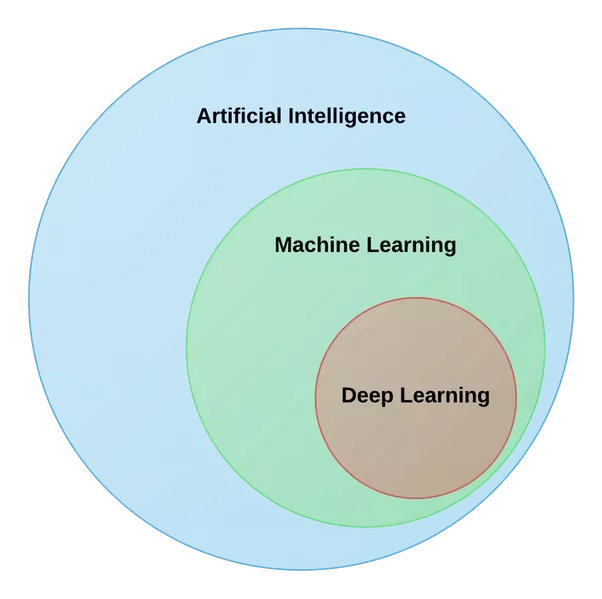
\includegraphics[width=0.44\textwidth]{Immagini/Generiche/AI_ML_DL_Differenze_v2.png}
    \caption{Rappresentazione delle categorie \cite{INGLOBAZIONE_IA}.} 
    \label{fig:rappresentazione dell'IA, ML e DL}
    %Figura 2.1: Esempio schematico di un neurone
\end{figure}
Ciascuna di queste discipline può essere vista come un elemento del livello precedente.
Il Machine Learning rappresenta un sottoinsieme dell’Intelligenza Artificiale. 
Il Deep Learning, a sua volta, è un sottoinsieme del Machine Learning e le 
reti neurali costituiscono l'elemento fondamentale degli 
algoritmi di Deep Learning.
Si può anche dire che l'Intelligenza Artificiale è la disciplina di base e il Machine 
Learning e il Deep Learning le tecniche che ne consentono 
l’applicazione \cite{IA_1,IA_ML_DL}. 


% \subsection{Cenni storici}
% Si può dire che l’AI nasce con l’avvento dei computer, nella seconda metà
% degli anni cinquanta. Il primo programma di un sistema intelligente riguardava solo la
% dimostrazione di alcuni teoremi matematici partendo da determinate informazioni. 
% Successivamente, molte università e aziende americane come l’IBM si
% cimentarono nello sviluppo di programmi e software in grado di pensare come
% gli esseri umani.
% Col passare degli anni vennero sviluppati software sempre più complicati
% dal punto di vista matematico ma, contrariamente a quello che si sperava,
% l’intelligenza artificiale sembrava non riuscire a riprodurre le caratteristiche
% intellettuali umane. Il progresso definitivo si ebbe con l’avvento delle reti
% neurali, che hanno permesso ai sistemi intelligenti di migliorare sempre di più
% le proprie capacità di comportamento. Ora, questi sistemi sono in grado di
% prendere decisioni senza l’intervento umano ed effettuare scelte a seconda del
% contesto in cui sono inseriti \cite{IA_1}.


\section{Machine Learning}
\subsection{Definizione}

Machine Learning comprende un insieme di metodi con cui si allena l’intelligenza artificiale 
a svolgere delle attività non programmate, a imparare dall’esperienza passata, 
come fa esattamente l’intelligenza umana, correggendosi 
e quindi migliorandosi attraverso gli errori commessi.
Questa disciplina viene chiamata anche apprendimento automatico, poiché il modello
impara dalla propria esperienza, senza la necessità di inserire 
nuove istruzioni \cite{IA_ML_DL}.

% Per fare ciò vengono usati algoritmi di regressione o di classificazione 
% per comprendere i dati a disposizione. 

\subsection{Le modalità dell’apprendimento}
Gli algoritmi di apprendimento automatico possono essere suddivisi i quattro categorie 
\cite{I_3_PROBLEMI_ML_e_APPRENDIMENTO, ASPETTI_ML}:
\begin{itemize}
    \item \textbf{Apprendimento supervisionato}: vengono presentati al modello una
    serie di esempi ideali costituiti dalla coppia input-output, in modo che
    riesca a capire la correlazione tra le entrate e le uscite.

    \item \textbf{Apprendimento non supervisionato}: al contrario dell’apprendimento
    precedente il modello riceve solo gli input. Deve capire da solo l’output
    da generare senza potersi confrontare con gli esempi dati.

    \item \textbf{Apprendimento per rinforzo}: Al programma viene fornito 
    un feedback per ogni azione che svolge. Un feedback positivo
    che si tradurrà in una ricompensa indica un’azione svolta correttamente,
    al contrario una punizione indicherà un’azione sbagliata.
    
    \item \textbf{Apprendimento semi-supervisionato}: vengono fornite informazioni
    incomplete sotto forma di esempi come nell’apprendimento supervisionato
    e il modello cercherà di prevedere anche quali sono i risultati mancanti.
\end{itemize}

\newpage
\subsection{Tipologie di problemi}
Nel Machine Learning, si possono distinguere tre tipologie di problemi
\cite{I_3_PROBLEMI_ML_e_APPRENDIMENTO, ASPETTI_ML}:

\begin{itemize}
    \item La \textbf{classificazione}, nella quale gli input sono divisi 
    in due o più classi e
    il sistema di apprendimento deve produrre un modello in grado di
    assegnare ad un input una o più classi tra quelle disponibili. Questi tipi
    di task sono tipicamente affrontati mediante tecniche di apprendimento
    supervisionato. Un esempio di classificazione è l’assegnamento di una
    o più etichette ad una immagine in base agli oggetti o soggetti contenuti
    in essa;
    
    \item La \textbf{regressione}, concettualmente simile alla classificazione con la
    differenza che l’output ha un dominio continuo e non discreto.
    Anch'essa è tipicamente affrontata con l’apprendimento supervisionato.

    \item Il \textbf{clustering}, nel quale, come nella classificazione, un insieme di dati
    viene diviso in gruppi che però, a differenza di questa, non sono noti a
    priori. La natura stessa dei problemi appartenenti a questa categoria li
    rende tipicamente dei task di apprendimento non supervisionato.
\end{itemize}


\section{Deep Learning}
\subsection{Definizione}
Il Deep Learning è un sottoinsieme del Machine Learning che si occupa
di analizzare i dati in maniera profonda, solitamente attraverso una rete di
apprendimento che prende decisioni e giunge a conclusioni in base ai dati forniti.
Questo metodo è particolarmente adatto a grandi set di dati, in quanto molto
più preciso, anche se molto più dispendioso in termini di risorse computazionali
e temporali rispetto all’apprendimento automatico.
% Il modello classico del Deep Learning è caratterizzato da gerarchie di
% caratteristiche comuni che mira ad andare in profondità nell’albero gerarchico
% tra i vari strati (per questo motivo viene detto "apprendimento profondo").
Tra i modelli di apprendimento automatico, trovano larga applicazione le reti 
neurali \cite{IA_ML_DL, ASPETTI_DEEP_LEARNING, ASPETTI_DEEP_LEARNING_2}.
% profonde, la convoluzione di reti neurali profonde e le reti neurali ricorsive, le
% quali vengono applicate nella visione artificiale, nel riconoscimento automatico
% del discorso, nell’elaborazione del linguaggio naturale, nel riconoscimento audio
% e nella bioinformatica 
% \cite{IA_ML_DL, ASPETTI_DEEP_LEARNING, ASPETTI_DEEP_LEARNING_2}.
    \section{I Dataset}
Spesso nella tesi useremo il termine \textbf{dataset} ("insieme di dati" in italiano). 
Questo termine viene utilizzato per riferirsi ad una collezione 
strutturata di dati, generalmente di grandi dimensioni e organizzata, correlati a 
un argomento, tema o settore specifico. 

I dataset possono includere diversi tipi di informazioni, come numeri, testo, 
immagini, video e audio, e possono essere archiviati in vari formati, 
come CSV, JSON, SQL o altri formati.

I dataset possono essere utilizzati per condurre ricerche di mercato, 
analizzare i concorrenti, confrontare i prezzi, identificare e studiare le 
tendenze o addestrare modelli di apprendimento automatico. Questi sono solo 
alcuni esempi e i dataset sono utili in varie aree e situazioni. Ad esempio, noi 
utilizzeremo dei dataset per "addestrare" delle reti neurali per uno specifico 
problema \cite{Dataset_Bright,Dataset_Wikipedia}.
\newpage
\subsection{Tipologie di dataset per il ML}
Quando si addestra un modello di ML, vengono utilizzati diversi dataset per 
applicazioni differenti \cite{UTILIZZI_DATASET}:

\begin{itemize}
    \item \textbf{Training Dataset}: è il dataset utilizzato per addestrare il 
    modello di Machine Learning. Durante questa fase, il modello apprende le 
    relazioni e i pattern nei dati.

    \item \textbf{Validation Dataset}: è utilizzato per monitorare il modello 
    durante l'addestramento e ridurre il rischio di overfitting, ovvero quando 
    il modello si adatta troppo bene ai dati di addestramento e 
    perde capacità di generalizzare.
    
    \item \textbf{Test Dataset}: è il dataset utilizzato dopo l'addestramento per 
    valutare le prestazioni finali del modello. Serve a confermare 
    che il modello generalizzi bene su dati completamente nuovi.
\end{itemize}

Questi dataset possono essere anche ottenuti partendo da uno stesso dataset, 
dividendo il dataset principale in diversi dataset più piccoli.
Tipicamente, dal dataset principale, si utilizza un 60-70\% per il training, un 10-20\% 
per la validation e un 10-20\% per il test \cite{DIVISIONE_DATASET,DIVISIONE_DATASET_2}.

\begin{figure}[H]
    \centering
    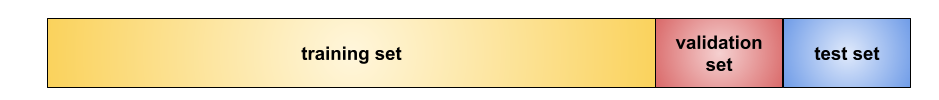
\includegraphics[width=1\textwidth]{Immagini/Generiche/PartitionThreeSets.png}
    \caption{Rappresentazione della suddivisione del dataset \cite{DIVISIONE_DATASET}.}
\end{figure}

    \newpage
\section{Valutazione dei modelli}
Quasi sempre quando si addestra un modello di ML, occorre un modo per valutare le 
sue prestazioni.

\subsection{La Matrice di confusione}
Una matrice di confusione (o matrice di errore) è un metodo di visualizzazione 
per i risultati dell'algoritmo di classificazione. Più specificamente, 
è una tabella che suddivide il numero di istanze di verità di base di una 
classe specifica rispetto al numero di istanze di classe previste.
In una matrice di confusione, le colonne rappresentano i valori previsti di una 
data classe, mentre le righe rappresentano i valori effettivi 
(ad esempio, le verità di base) di una data classe, o viceversa.
Questa struttura a griglia è uno strumento utile per visualizzare l'accuratezza 
della classificazione dei modelli. In quanto permette di visualizzare 
il numero di previsioni corrette e previsioni errate per tutte le classi una 
accanto all'altra
\cite{Confusion_Matrix_e_metrics1,Confusion_Matrix_e_metrics2}.

Un modello di matrice di confusione standard per un classificatore 
binario può essere simile a:

\begin{figure}[H]
    \centering
    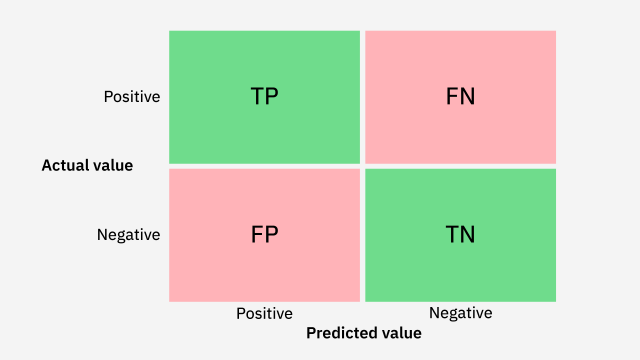
\includegraphics[width=0.60\textwidth]{Immagini/Grafici/esempio_MC_1.png}
    \caption{Esempio di una matrice di confusione per classificazione binaria
    \cite{Confusion_Matrix_e_metrics1} .}
\end{figure}

La casella in alto a sinistra fornisce il numero di veri positivi (TP), ovvero 
il numero di previsioni corrette per la classe positiva. Il riquadro sottostante è 
rappresentato dai falsi positivi (FP), ovvero quei casi di classe negativa erroneamente 
identificati come casi positivi. In statistica, questi sono anche chiamati errori 
di tipo I. La casella in alto a destra indica il numero di falsi negativi (FN), 
i casi effettivamente positivi erroneamente previsti come negativi. Infine, nella 
casella in basso a destra viene visualizzato il numero di veri negativi (TN), 
ovvero le istanze effettive della classe negativa previste con precisione. 
Sommando ciascuno di questi valori si otterrebbe il numero totale di previsioni 
del modello \cite{Confusion_Matrix_e_metrics1,Confusion_Matrix_e_metrics2}.

% Naturalmente, questo modello è per un rudimentale problema di classificazione 
% binaria. La matrice di confusione può visualizzare i risultati anche per 
% problemi di classificazione multiclasse. 
% Ad esempio, immaginiamo di sviluppare un 
% modello di classificazione delle specie come parte di un programma di conservazione 
% della vita marina. Il modello prevede le specie ittiche. 
\newpage
Una matrice di confusione può essere utilizzata anche per problemi di 
classificazione multiclasse. 
%di questo tipo può essere simile alla seguente:

\begin{figure}[H]
    \centering
    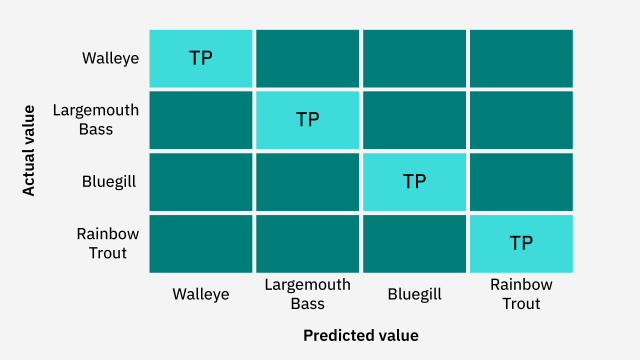
\includegraphics[width=0.70\textwidth]{Immagini/Grafici/esempio_MC_2.png}
    \caption{Esempio di una matrice di confusione per classificazione multi classe}
    %\label{fig:rappresentazione dell'IA, ML e DL}
    %Figura 2.1: Esempio schematico di un neurone
\end{figure}

Tutte le caselle diagonali indicano i veri positivi previsti. 
Le altre caselle forniscono le quantità per i falsi positivi, i falsi 
negativi ed i veri negativi a seconda della classe che si sceglie di mettere a fuoco.
La matrice di confusione può servire a calcolare diverse metriche di valutazione, 
come per esempio il tasso di errore, l’accuratezza, la precisione, 
il richiamo o sensibilità (Recall) e l’F1-score.
Mettendo la matrice di confusione e le metriche ad essa associate sotto osservazione, 
è possibile identificare le aree in cui il modello presenta criticità. 
Così è possibile adottare misure specifiche per aumentare la precisione 
delle previsioni \cite{Confusion_Matrix_e_metrics1,Confusion_Matrix_e_metrics2}.

\subsection{L'accuratezza}

% L’accuratezza rappresenta la percentuale di predizioni corrette 
% rispetto al totale delle predizioni. L'accuratezza varia da 0 (scenario peggiore) 
% a 1 (previsione migliore).

L'accuratezza rappresenta la percentuale di predizioni corrette 
rispetto al totale delle predizioni effettuate. Questo valore 
varia da 0, che rappresenta lo scenario peggiore in cui tutte le predizioni sono errate, 
a 1, che corrisponde alla massima accuratezza con tutte le predizioni corrette.
L'accuratezza si calcola utilizzando la seguente formula:

\begin{equation}
    \text{ACC} = \frac{\text{Casi corretti}}{\text{Numero totale di casi}}=\frac{TP + TN}{TP+TN+FP+FN}
\end{equation}

Tuttavia, l'accuratezza del modello non è una metrica di valutazione completamente 
informativa per i classificatori. Immaginiamo, ad esempio, di eseguire un 
classificatore su un set di dati di 100 istanze. La matrice di confusione 
del modello mostra solo un falso negativo e nessun falso positivo; 
il modello classifica correttamente ogni altra istanza di dati. 
Pertanto, il modello ha una precisione del 99\%. 
Sebbene apparentemente desiderabile, l'elevata precisione non è di per sé 
indicativa di eccellenti prestazioni del modello. 
Ad esempio, supponiamo che il nostro modello miri a classificare malattie 
altamente contagiose. Questa errata classificazione dell'1\% rappresenta un 
rischio enorme. Pertanto, è possibile utilizzare altre metriche di valutazione 
per fornire un quadro migliore delle prestazioni dell'algoritmo di classificazione
\cite{Confusion_Matrix_e_metrics1,Confusion_Matrix_e_metrics2}.

\subsection{Precisione e richiamo}
La precisione è la proporzione di stime di classe positive che 
appartengono effettivamente alla classe in questione. 
Un altro modo per comprendere la precisione è che misura la probabilità 
che un'istanza scelta a caso appartenga ad una certa classe. La precisione può 
anche essere chiamata valore previsto positivo (PPV) 
\cite{Confusion_Matrix_e_metrics1,Confusion_Matrix_e_metrics2} . 
È rappresentato dall'equazione:

\begin{equation}
    \text{Precisione} = \frac{TP}{TP + FP}
\end{equation}

Mentre il richiamo indica la percentuale di istanze di classe rilevate da un modello.
In altre parole, indica la percentuale di previsioni positive per una data 
classe rispetto a tutte le istanze effettive di quella classe
\cite{Confusion_Matrix_e_metrics1,Confusion_Matrix_e_metrics2}. 
Il richiamo è noto anche come sensibilità o tasso di veri positivi ed è 
rappresentato dall'equazione:

\begin{equation}
    \text{Richiamo} = \frac{TP}{TP+FN}
\end{equation}

\subsection{F1 score}
F1 score, chiamato anche \textit{F-score}, \textit{F-measure} o 
\textit{media armonica di precisione e richiamo}, combina precisione e 
richiamo per rappresentare l'accuratezza totale 
di un modello rispetto alla classe. Utilizzando questi due valori, 
si può calcolare l'F1 score con l'equazione, in cui P indica la precisione 
(PPV) e R indica il richiamo (sensibilità):

\begin{equation}
    F = \frac{2PR}{P+R}
\end{equation}

F1 score è particolarmente utile per set di dati sbilanciati, 
in cui il compromesso tra precisione e richiamo può essere più evidente. 
Ad esempio, supponiamo di avere un classificatore che prevede la probabilità 
di una malattia rara. Un modello previsionale in cui nessuno nel nostro set di 
dati di test risulta affetto dalla malattia può avere una precisione perfetta ma 
zero richiami. Nel frattempo, un modello che preveda che tutti i soggetti del 
nostro set di dati siano affetti dalla malattia restituirebbe un richiamo 
perfetto ma una precisione pari alla percentuale di persone effettivamente 
affette dalla malattia (ad esempio 0,00001\% se solo uno su dieci milioni ha la malattia). 
F1 score è un mezzo per bilanciare questi due valori per ottenere una visione più 
olistica delle prestazioni di un classificatore \cite{Confusion_Matrix_e_metrics1,Confusion_Matrix_e_metrics2}.



    %%==========[CAPITOLO II]==========%%
    
\chapter{Frameworks e linguaggi di programmazione utilizzati}

\section{Il linguaggio Python}

\begin{wrapfigure}[6]{l}{0.13\textwidth}  % Specifica la larghezza dell'immagine e il numero di righe da avvolgere
    \setlength{\fboxsep}{1pt} % Distanza tra l'immagine e il bordo
    \setlength{\fboxrule}{0pt} % Spessore del bordo
    \fbox{
\includegraphics[width=0.11\textwidth]{Immagini/Loghi/Python-logo.png}}  % Aggiungi il logo con contorno
\end{wrapfigure}

Per la realizzazione dei vari esperimenti e illustrazioni esposti nel corso della
tesi, è stato utilizzato il linguaggio di programmazione Python, un linguaggio di 
programmazione utilizzato per lo sviluppo dell’analisi empirica. 
Python è un linguaggio di programmazione ad alto livello noto per la 
sua: dinamicità, semplicità e flessibilità.
Esso è un linguaggio interpretato in grado di supportare paradigmi di 
programmazione come: la programmazione procedurale, la programmazione orientata agli 
oggetti e la programmazione funzionale.
Vanta la possibilità di interfacciarsi con diversi tipi di system call, librerie e 
sistemi a finestra ed è estensibile in C o C++. Può anche essere utilizzato come linguaggio di 
estensione per applicazioni che necessitano di un’interfaccia programmabile. Python è in 
grado di combinare un potenziale notevole ad una sintassi molto chiara e infine si tratta di 
un linguaggio portatile: funziona su molte varianti di Unix, su MacOS e su Windows 
La nascita del linguaggio è attribuibile a Guido van Rossum, programmatore 
olandese laureatosi all’Università di Amsterdam con un Master in Matematica ed 
Informatica e conosciuto come il Benevolent Dictator for Life di Python. 
Con il tempo, Python, è diventato uno tra i più utilizzati
linguaggi di programmazione per l'ambito della \textit{data science} e 
\textit{data analytics}, con la crescente diffusione di progetti legati al 
Machine learning, Cloud computing e Big data. Ciò grazie anche
alla vasta raccolta di librerie \cite{Python_Wikipedia}.

Per la realizzazione dei vari programmi, alcune delle principali librerie che sono 
state utilizzate sono: %l'analisi dei dati sono:
\begin{itemize}
    \item \textbf{Numpy}, una libreria che fornisce supporto per array multidimensionali e 
    funzioni matematiche ad alte prestazioni per operare su di esse. 
    È particolarmente utile per manipolare grandi quantità di dati numerici in 
    modo efficiente;

    \item \textbf{Matplotlib} è una libreria per la visualizzazione dei dati. Consente di 
    realizzare grafici a linee, istogrammi, scatter plot e altro ancora;
    
    \item \textbf{Seaborn} è una libreria basata su Matplotlib che offre un'interfaccia più 
    intuitiva per la realizzazione di grafici statisticamente informativi, come le heatmap e 
    le matrici di confusione. 
    
    \item \textbf{Scikit-learn} è una libreria per l'apprendimento automatico. Fornisce una 
    vasta raccolta di strumenti per la classificazione, la regressione e il 
    clustering;

    \item \textbf{Pandas} è una libreria progettata per la manipolazione e l'analisi dei dati strutturati;
 
    \item \textbf{Pytorch} è una libreria open-source per l'apprendimento automatico e 
    il deep learning. Fornisce strumenti per creare reti neurali e algoritmi di 
    apprendimento basati su tensori.
\end{itemize}



\section{Frameworks per lo sviluppo di reti neurali}
Le reti neurali artificiali hanno dimostrato di essere all'avanguardia 
in molti casi di apprendimento supervisionato, ma programmare manualmente 
una rete neurale può essere un compito impegnativo. 
% Di conseguenza, sono stati 
% creati framework come TensorFlow e PyTorch per semplificare la creazione, 
% il servizio e la scalabilità dei modelli di deep learning.
Con l'aumento dell'interesse per il deep learning negli ultimi anni, 
si è assistito a un'esplosione di strumenti di apprendimento automatico. 
Negli ultimi anni sono stati introdotti e sviluppati a ritmo sostenuto 
framework di deep learning come PyTorch, TensorFlow, Keras, Chainer e altri.

\begin{figure}[H]
    \centering
    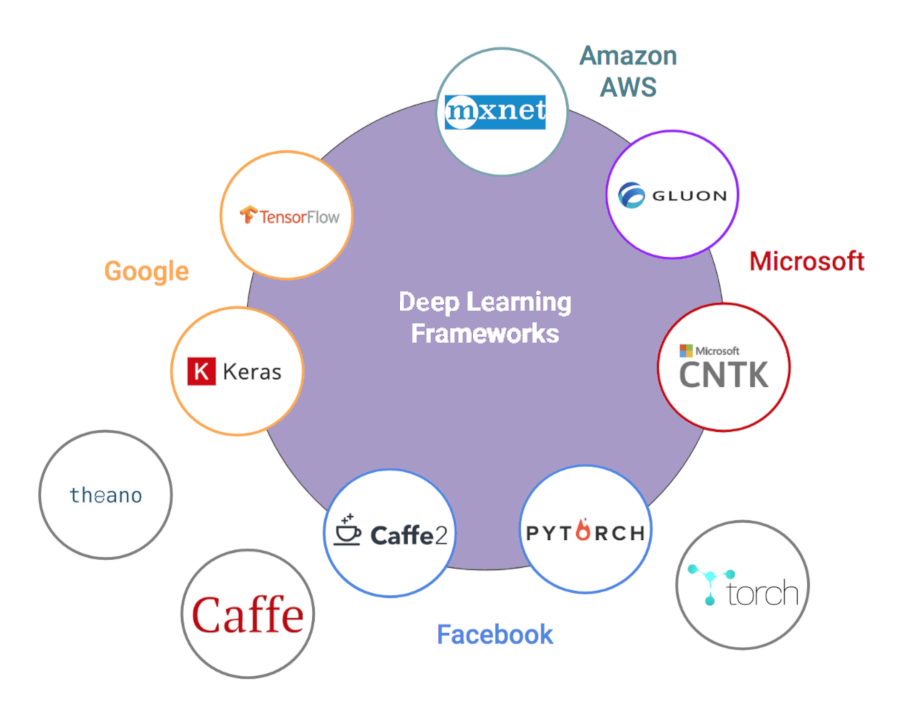
\includegraphics[width=0.55\textwidth]{Immagini/Generiche/Deep Learning Frameworks.png}
    \caption{Alcuni dei principali framework \cite{Framework_Devopedia}.}
\end{figure}

Questi framework forniscono unità di rete neurale, funzioni di costo e 
ottimizzatori per assemblare e addestrare modelli di rete neurale, permettendo di
semplificare e velocizzare lo sviluppo di questi modelli.
Alcuni di questi frameworks come Tensorflow, PyTorch e Keras; Sono disponibili
per il linguaggio di programmazione Python, sotto forma di libreria, fornendo un
API per la progettazione e l’addestramento di modelli.  


\subsection{Trends dei frameworks}

\begin{figure}[H]
    \centering
    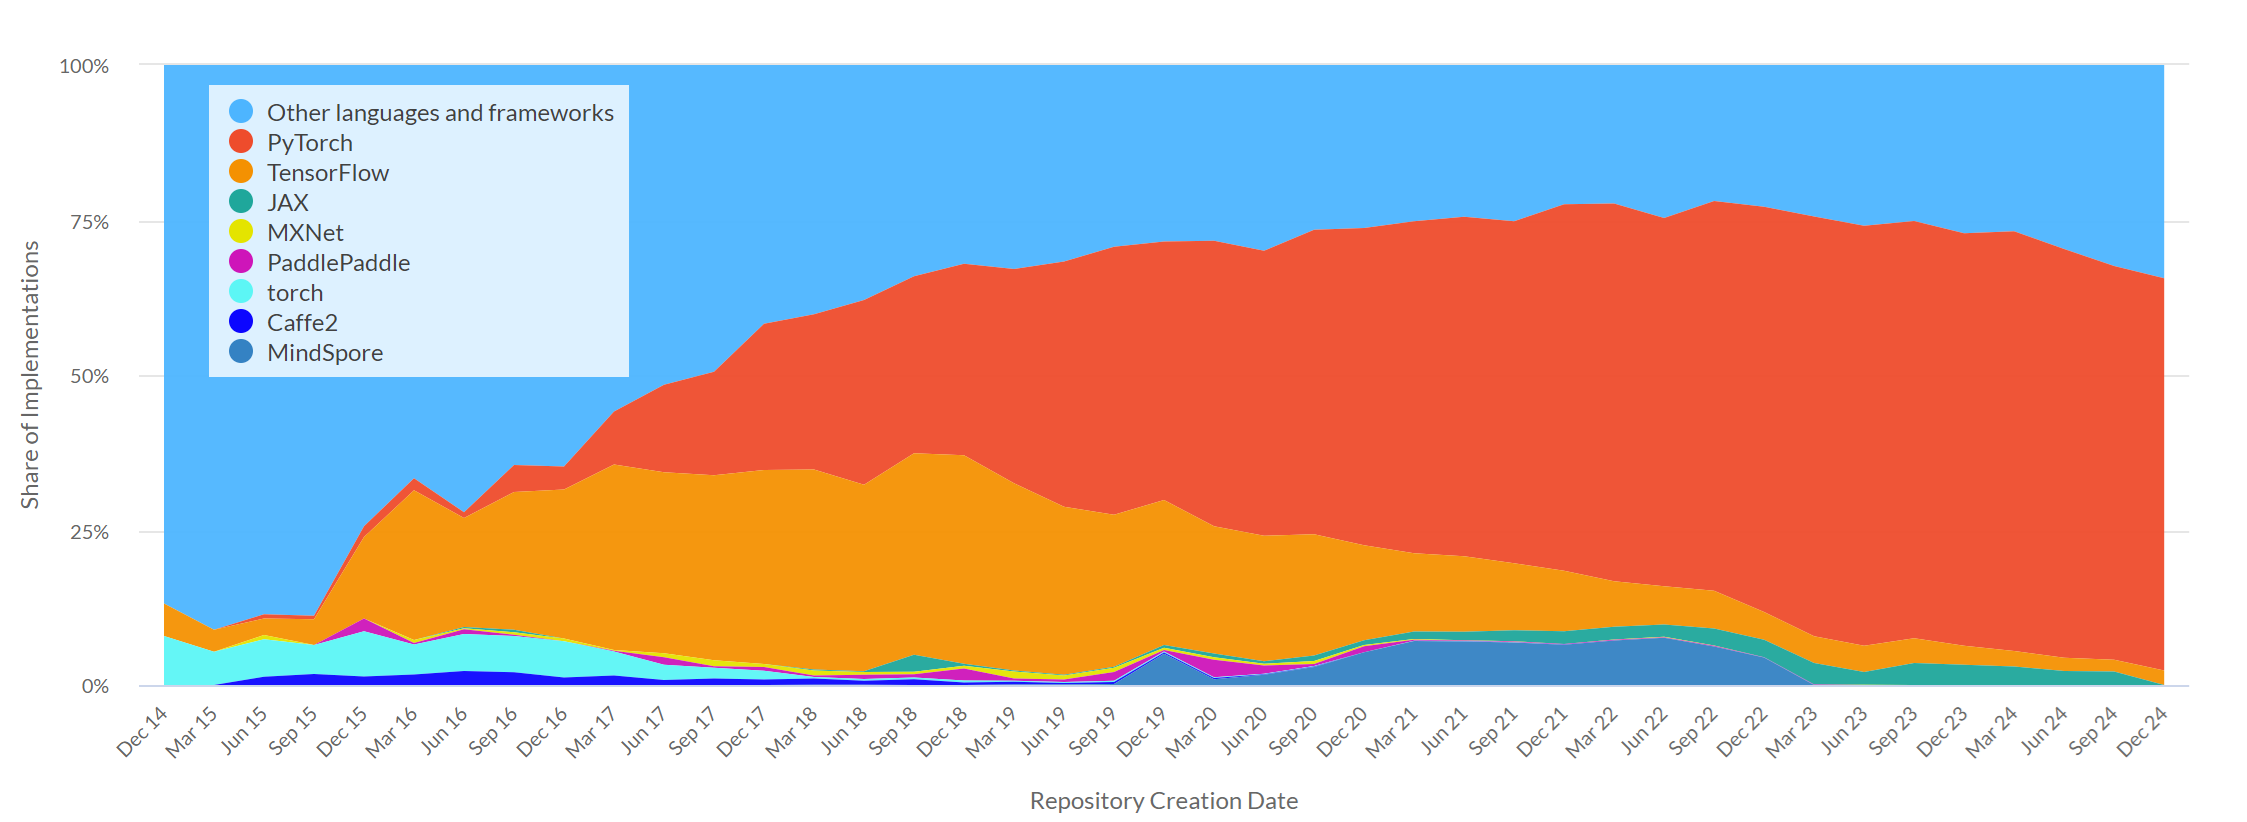
\includegraphics[width=1.0\textwidth]{Immagini/Grafici/graficoFrameWork.png}
    \caption{Trends dei frameworks \cite{Framework_PapersWithCode}.}
\end{figure}

Il grafico mostra l'andamento dei framework utilizzati nei repository GitHub 
dedicati alle implementazioni di articoli scientifici.
L'asse temporale indica la data di creazione dei repository, consentendo di 
osservare come la popolarità dei vari framework sia cambiata nel tempo.
Tra i più utilizzati spiccano TensorFlow e PyTorch, due strumenti fondamentali e 
molto apprezzati nel campo dell'apprendimento automatico.
Pertanto, per la realizzazione delle reti neurali, utilizzeremo Pytorch, in quanto è uno 
dei migliori framework per chi si avvicina per la prima volta a questo ambito. 



\subsection{TensorFlow}
% TensorFlow wrapfigure
\begin{wrapfigure}[6]{l}{0.25\textwidth}  % Specifica la larghezza dell'immagine e il numero di righe da avvolgere
    \setlength{\fboxsep}{1pt} % Distanza tra l'immagine e il bordo
    \setlength{\fboxrule}{0pt} % Spessore del bordo
    \fbox{
\includegraphics[width=0.23\textwidth]{Immagini/Loghi/Tensorflow_v2.png}}  % Aggiungi il logo con contorno
\end{wrapfigure}

Tensorflow \cite{Framework_AnalyticsVidhya,Framework_VisoAI,Framework_Devopedia} è una libreria open source sviluppata da Google che fornisce risorse per la creazione di modelli per l’apprendimento automatico.  
Rilasciata ufficialmente nel 2015, è diventata velocemente una delle più popolari soprattutto grazie 
al supporto per diversi linguaggi di programmazione, come Python, C++ e R.
In oltre dispone di un'ottima documentazione e linee guida,che la rendono un’ottima scelta per chi si avvicina per la prima volta a tale mondo.  

Tra i principali vantaggi, TensorFlow offre:
\begin{itemize}
    \item Supporto per l’esecuzione su GPU e TPU, che permette di accelerare i tempi di addestramento.
    \item Un ecosistema completo, che include TensorBoard per la visualizzazione e TensorFlow Lite per l’ottimizzazione su dispositivi mobili.
\end{itemize}
\aftergroup
\par
\subsection{Keras}
% Keras wrapfigure
\begin{wrapfigure}[4]{l}{0.25\textwidth}  % Specifica la larghezza dell'immagine e il numero di righe da avvolgere
    \setlength{\fboxsep}{2pt} % Distanza tra l'immagine e il bordo
    \setlength{\fboxrule}{0pt} % Spessore del bordo
    \fbox{
\includegraphics[width=0.22\textwidth]{Immagini/Loghi/Kerass.png}}  % Aggiungi il logo con contorno
\end{wrapfigure}

Keras \cite{Framework_AnalyticsVidhya,Framework_VisoAI,Framework_Devopedia} è 
una libreria open source scritta in Python e può essere eseguita su 
TensorFlow (oltre che su CNTK e Theano). L'interfaccia di TensorFlow può essere un 
po' ostica, poiché si tratta di una libreria di basso livello e i nuovi utenti 
potrebbero avere difficoltà a comprendere alcune implementazioni.
Keras, invece, è un'API di alto livello, sviluppata con l'obiettivo di consentire 
una sperimentazione rapida. Quindi, se si vogliono ottenere risultati rapidi, 
Keras si occuperà automaticamente dei compiti principali e genererà l'output.

\aftergroup
\par

\subsection{Pytorch}
% PyTorch wrapfigure
\begin{wrapfigure}[4]{l}{0.28\textwidth}  % Specifica la larghezza dell'immagine e il numero di righe da avvolgere
    \setlength{\fboxsep}{2pt} % Distanza tra l'immagine e il bordo
    \setlength{\fboxrule}{0pt} % Spessore del bordo
    \fbox{
\includegraphics[width=0.25\textwidth]{Immagini/Loghi/PyTorch_logo_black.png}}  % Aggiungi il logo con contorno
\end{wrapfigure}

PyTorch \cite{Framework_AnalyticsVidhya,Framework_VisoAI,Framework_Devopedia} è una libreria open source sviluppata da Facebook e introdotta per la 
prima volta nel 2016. Questa libreria è particolarmente apprezzata per la 
sua flessibilità con un'attenta considerazione delle prestazioni e per l'approccio 
dinamico al calcolo dei grafi computazionali. Oggi, la maggior parte del suo nucleo è scritto in C++, uno dei motivi principali 
per cui PyTorch può ottenere un overhead molto più basso rispetto ad 
altri framework. Ad oggi, PyTorch sembra essere il più adatto a ridurre 
drasticamente il ciclo di progettazione, addestramento e test di nuove reti 
neurali per scopi specifici. Per questo è diventato molto popolare nelle comunità 
di ricerca.

\subsection{PyTorch Lightning}

\begin{wrapfigure}[4]{l}{0.30\textwidth}  % Specifica la larghezza dell'immagine e il numero di righe da avvolgere
    \setlength{\fboxsep}{2pt} % Distanza tra l'immagine e il bordo
    \setlength{\fboxrule}{0pt} % Spessore del bordo
    \fbox{
\includegraphics[width=0.28\textwidth]{Immagini/Loghi/Lightning_Logo.png}}  % Aggiungi il logo con contorno
\end{wrapfigure}

PyTorch Lightning \cite{PyTorchLightning, PyTorchLightning_site} è una libreria Python 
open-source che fornisce un'interfaccia di 
alto livello per PyTorch. È un framework leggero e ad alte prestazioni che 
organizza il codice PyTorch per disaccoppiare la ricerca dall'ingegneria, rendendo 
così gli esperimenti di deep learning più facili da leggere e riprodurre,
accelerando così i tempi di sviluppo dei modelli. 
È stato progettato per creare modelli scalabili di deep learning che possono 
essere facilmente eseguiti su hardware distribuito.
In oltre, PyTorch Lightning possiede una struttura modulare che semplifica 
la gestione di training, validazione e logging.
\aftergroup
\par
    \section{Il tensore}
Quando si lavora con gli algoritmi di machine learning, spesso occorre un modo per
rappresentare numericamente informazioni complessi come: suoni, immagini, testo o 
altre informazioni. 
In framework di machine learning e deep learning come TensorFlow e PyTorch,
la rappresentazione numerica delle informazioni è ottenuta attraverso
l'uso dei \textbf{Tensori}, che fungono da unità fondamentale 
per il calcolo sulla piattaforma. 

Un Tensore può essere definito come un oggetto matematico, una struttura dati 
multidimensionale che generalizza il concetto di scalare, vettore e 
matrice a $n$-dimensioni. Nel contesto della \textit{data science}, i tensori 
sono matrici multidimensionali di numeri che rappresentano dati complessi
\cite{Tensore_Fidacaro,Tensore_IBM,tensor_analytic,tensor_medium1,tensor_medium2,tensor_strano}. 

\subsection{Struttura e Caratteristiche dei Tensori}
Un tensore è definito da due proprietà principali che ne determinano la 
struttura \cite{Tensore_Fidacaro} :

\begin{itemize}
    \item \textbf{Rank (o dimensione)}:  
    Il rank di un tensore indica il numero di assi o direzioni lungo cui i dati 
    sono organizzati.
    
    \item \textbf{Shape (o forma)}:  
    La shape di un tensore è una tupla che specifica il numero di elementi lungo ogni asse. 
\end{itemize}

\subsection{Rappresentazione dei dati}
A seconda della loro dimensione (rank) e della forma (shape), i tensori possono modellare 
dati di diversa natura \cite{Tensore_Fidacaro}:

\begin{itemize}
    \item \textbf{Scalare}: Un tensore scalare rappresenta un singolo valore numerico. 
    Non ha direzioni o assi, ed è quindi di dimensione 0. 
    Ad esempio potrebbe essere il numero $5.5$ . 

    \item \textbf{Vettore}: Un vettore, ad esempio $[1\ 2\ 3]$, è una sequenza ordinata 
    di numeri disposti lungo un unico asse, e può essere rappresentato da un tensione di 
    dimensione 1.
  
    \item \textbf{Matrice}: una matrice come $\begin{bmatrix} 1 & 2 & 3 \\ 4 & 5 & 6 \end{bmatrix}$ 
    può essere vista come un tensore di dimensione 2.

    \item \textbf{Strutture 3D e oltre}: tutte le strutture matematiche con tre o più dimensioni, 
    ad esempio come 
    $\begin{bmatrix} 
    \begin{bmatrix} 1 & 2 \\ 3 & 4 \end{bmatrix} & 
    \begin{bmatrix} 5 & 6 \\ 7 & 8 \end{bmatrix} 
    \end{bmatrix}$, vengono rappresentati come tensori di dimensione 3 o superiore.
\end{itemize}

La figura (\ref{fig:Rappresentazione_Tensori}) mostra una rappresentazione grafica dei tensori al variare 
della dimensione

\begin{figure}[H]
    \centering
    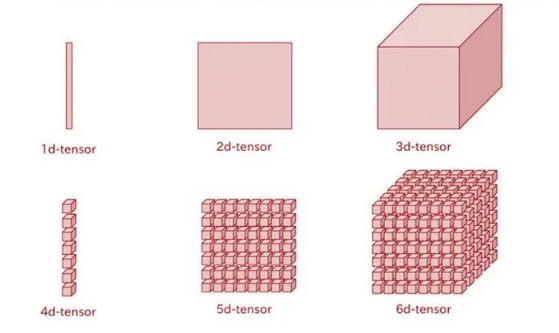
\includegraphics[width=0.72\textwidth]{Immagini/Generiche/esempio_tensori.png}
    \caption{Rappresentazione grafica dei tensori \cite{tensor_medium2} .}
    \label{fig:Rappresentazione_Tensori}
    %Figura 2.1: Esempio schematico di un neurone
\end{figure}


Ad esempio, se volessi utilizzare in python un tensore di pytorch per rappresentare 2 immagini 
RGB 3x3, il tensore apparirebbe così:
\begin{lstlisting}
images = torch.tensor([
    [
        [[255, 0, 0], [255, 255, 0], [0, 255, 0]], 
        [[0, 0, 255], [0, 255, 255], [0, 0, 255]], 
        [[255, 255, 255], [128, 128, 128], [0, 0, 0]]
    ], 
    [
        [[0, 0, 0], [128, 128, 128], [255, 255, 255]], 
        [[255, 0, 255], [255, 255, 0], [0, 255, 0]], 
        [[0, 0, 255], [255, 255, 255], [128, 128, 128]]
    ] 
])
\end{lstlisting}
Questo tensore così creato avrebbe shape $(2, 3, 3, 3)$ .


% \section{Operazioni tra tensori}
% Le operazioni sui tensori generalizzano quelle tra numeri, vettori e matrici. Tra le operazioni più comuni troviamo:

% \subsubsection{1. Somma tra tensori}
% Due tensori possono essere sommati solo se hanno la stessa forma (dimensioni). La somma viene eseguita elemento per elemento.

% \begin{itemize}
%     \item \textbf{Tensore A:} $\begin{bmatrix} 1 & 2 \\ 3 & 4 \end{bmatrix}$
%     \item \textbf{Tensore B:} $\begin{bmatrix} 5 & 6 \\ 7 & 8 \end{bmatrix}$
%     \item \textbf{Somma A + B:} $\begin{bmatrix} 1+5 & 2+6 \\ 3+7 & 4+8 \end{bmatrix} = \begin{bmatrix} 6 & 8 \\ 10 & 12 \end{bmatrix}$
% \end{itemize}

% \subsubsection{2. Moltiplicazione elemento per elemento (Hadamard product)}
% Due tensori con la stessa forma possono essere moltiplicati elemento per elemento.

% \begin{itemize}
%     \item \textbf{Tensore A:} $\begin{bmatrix} 1 & 2 \\ 3 & 4 \end{bmatrix}$
%     \item \textbf{Tensore B:} $\begin{bmatrix} 5 & 6 \\ 7 & 8 \end{bmatrix}$
%     \item \textbf{Prodotto Hadamard AB:} $\begin{bmatrix} 1 \cdot 5 & 2 \cdot 6 \\ 3 \cdot 7 & 4 \cdot 8 \end{bmatrix} = \begin{bmatrix} 5 & 12 \\ 21 & 32 \end{bmatrix}$
% \end{itemize}

% \subsubsection{3. Prodotto scalare (dot product)}
% Il prodotto scalare tra due tensori è possibile quando una delle dimensioni del primo tensore corrisponde a una delle dimensioni del secondo.

% \begin{itemize}
%     \item \textbf{Tensore A (2x3):} $\begin{bmatrix} 1 & 2 & 3 \\ 4 & 5 & 6 \end{bmatrix}$
%     \item \textbf{Tensore B (3x2):} $\begin{bmatrix} 7 & 8 \\ 9 & 10 \\ 11 & 12 \end{bmatrix}$
%     \item \textbf{Prodotto A · B:} 
%     $\begin{bmatrix} 
%     (1 \cdot 7 + 2 \cdot 9 + 3 \cdot 11) & (1 \cdot 8 + 2 \cdot 10 + 3 \cdot 12) \\ 
%     (4 \cdot 7 + 5 \cdot 9 + 6 \cdot 11) & (4 \cdot 8 + 5 \cdot 10 + 6 \cdot 12) 
%     \end{bmatrix} = \begin{bmatrix} 58 & 64 \\ 139 & 154 \end{bmatrix}$
% \end{itemize}

% \subsubsection{4. Prodotto tensore (tensor product)}
% Il prodotto tensore tra due tensori crea un tensore di ordine più alto.

% \begin{itemize}
%     \item \textbf{Tensore A:} $[1, 2]$
%     \item \textbf{Tensore B:} $[3, 4]$
%     \item \textbf{Prodotto AB:} $\begin{bmatrix} 1 \cdot 3 & 1 \cdot 4 \\ 2 \cdot 3 & 2 \cdot 4 \end{bmatrix} = \begin{bmatrix} 3 & 4 \\ 6 & 8 \end{bmatrix}$
% \end{itemize}

% \subsubsection{5. Trasposizione}
% La trasposizione di un tensore consiste nello scambiare l'ordine di alcune delle sue dimensioni. Per esempio, in una matrice, si scambiano righe e colonne.

% \begin{itemize}
%     \item \textbf{Tensore A:} $\begin{bmatrix} 1 & 2 & 3 \\ 4 & 5 & 6 \end{bmatrix}$
%     \item \textbf{Trasposta $A^T$:} $\begin{bmatrix} 1 & 4 \\ 2 & 5 \\ 3 & 6 \end{bmatrix}$
% \end{itemize}

% \subsubsection{6. Riduzione di dimensioni}
% I tensori possono essere ridotti lungo una determinata dimensione, sommando o calcolando la media degli elementi.

% \begin{itemize}
%     \item \textbf{Tensore A (2x3):} $\begin{bmatrix} 1 & 2 & 3 \\ 4 & 5 & 6 \end{bmatrix}$
%     \item \textbf{Somma lungo la prima dimensione:} $[1+4, 2+5, 3+6] = [5, 7, 9]$
%     \item \textbf{Somma lungo la seconda dimensione:} $[1+2+3, 4+5+6] = [6, 15]$
% \end{itemize}

\subsection{I tensori nelle reti neurali}
Come si vedrà più avanti, il funzionamento delle reti neurali si basa 
su delle operazioni matematiche lineari, come ad esempio il prodotto matriciale. 
I tensori funzionano in modo simile ai \textit{ndarray} usati in NumPy, ma a 
differenza dei \textit{ndarray}, che possono essere eseguiti solo su unità 
di elaborazione centrali (CPU), i tensori possono essere eseguiti anche
su appositi acceleratori hardware, come le unità di elaborazione grafica (GPU) e 
unità di elaborazione per Tensori (TPU) .
Le GPU e TPU consentono un calcolo notevolmente più veloce rispetto alle CPU, 
il che rappresenta un grande vantaggio dati gli enormi volumi di dati e 
l'elaborazione parallela tipici del deep learning.
Riassumendo, utilizzare i tensori per rappresentare le informazioni e 
svolgere calcoli, permette di sfruttare l'accelerazione hardware 
offerta da GPU e TPU per parallelizzare le operazioni matematiche e 
svolgerle in modo efficiente.
I tensori, oltre ad essere utilizzati per codificare gli input e gli output 
di un modello di una rete neurale, vengono utilizzati anche per 
codificare i parametri del modello: pesi, pregiudizi e gradienti che 
vengono "appresi". 
Questa proprietà dei tensori consente la differenziazione automatica 
(calcolo automatico delle derivate), una delle funzioni più importanti 
di PyTorch \cite{Tensore_Fidacaro,Tensore_IBM,tensor_analytic,tensor_medium1,tensor_medium2,tensor_strano}.

\subsection{Velocità computazionale dei tensori}
Per dare idea dei vantaggi computazionali dell'utilizzo dei tensori, 
realizziamo un test in cui confrontiamo le prestazioni degli array \textit{NumPy}
e dei tensori di \textit{PyTorch} nella moltiplicazione tra matrici.
In questo test inizializziamo casualmente  due \textit{arrays/tensors} 4D
e misureremo il tempo necessario a svolgere la moltiplicazione tra i due.
Come dispositivo di accelerazione hardware utilizzeremo una GPU, la cui 
selezione avviene tramite il comando \texttt{torch.device("cuda")}.
Qualora si volesse selezionare una specifica GPU, è possibile aggiungere un numero dopo 
\texttt{"cuda"} il numero della GPU (ad esempio \texttt{"cuda:1"} per selezionare la 
seconda GPU). Se il numero viene omesso, il comando utilizzerà automaticamente 
la GPU \texttt{"cuda:0"}. Il codice del test è il seguente:

\begin{lstlisting}
import torch
import numpy as np
import time

dim_max = 110
shapes = []
device = torch.device("cuda")

for dim in range(5, dim_max + 1, 5):
    shapes.append((dim, dim, dim, dim))

for shape in shapes:
    array1 = np.random.rand(*shape)
    array2 = np.random.rand(*shape)
    tensor1 = torch.rand(*shape).to(device)
    tensor2 = torch.rand(*shape).to(device)

    start_time = time.perf_counter()
    np.matmul(array1, array2)
    dt = time.perf_counter() - start_time
    cpu_times.append(dt)

    torch.cuda.synchronize() 
    start_time = time.perf_counter()
    torch.matmul(tensor1, tensor2)
    torch.cuda.synchronize()
    gpu_times.append(time.perf_counter() - start_time)
plot(shapes, cpu_times, gpu_times)

\end{lstlisting}

Eseguito il test di confronto, questi sono i risultati che otteniamo: 

\begin{figure}[H]
    \centering
    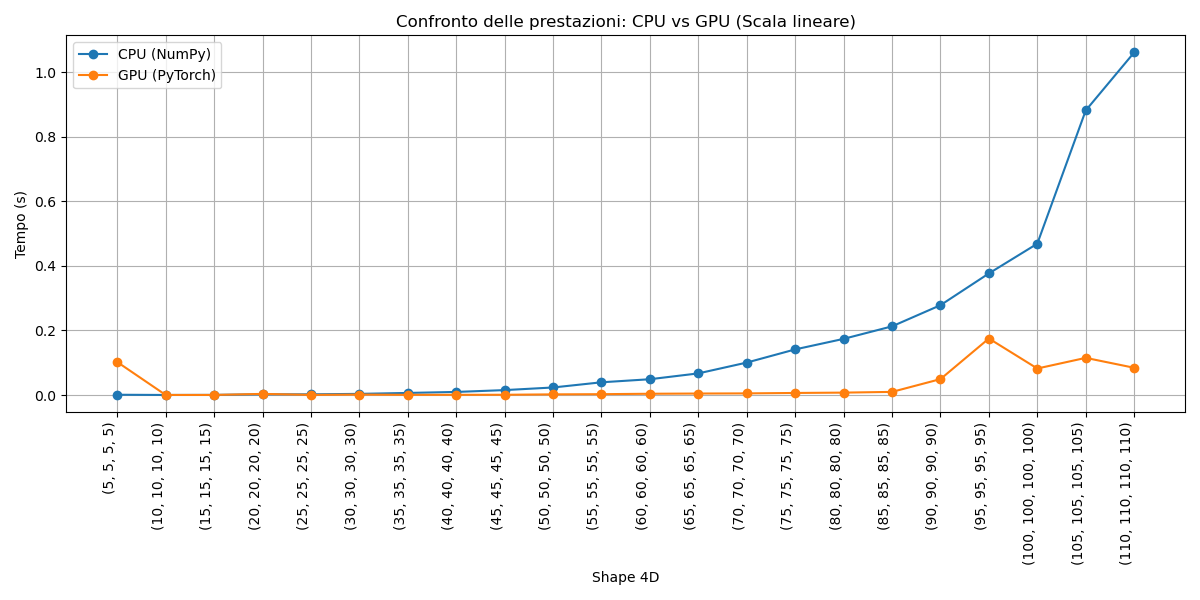
\includegraphics[width=0.92\textwidth]{Immagini/Grafici/Tensor_lin_plot.png}
    \caption{Grafico lineare del paragone array-tensore }
\end{figure}

\begin{figure}[H]
    \centering
    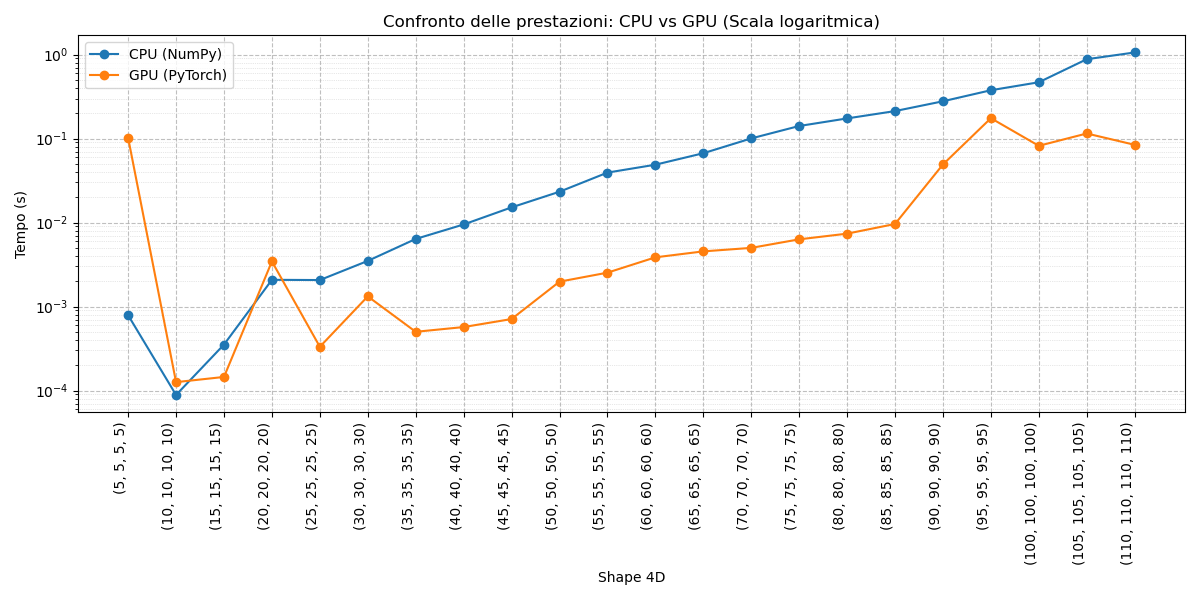
\includegraphics[width=0.92\textwidth]{Immagini/Grafici/Tensor_log_plot.png}
    \caption{Grafico logaritmico del paragone array-tensore }
\end{figure}
 

Come possiamo osservare, per dimensioni ridotte, i calcoli eseguiti con gli array
di \textit{NumPy} risultano essere molto più veloci rispetto a quelli svolti 
con i tensori di \textit{PyTorch}.
Ma all'aumentare delle dimensioni, i calcoli eseguiti su GPU 
risultano essere da 24 a 52 volte più veloci rispetto a quelli su CPU.
Le prestazioni possono dipendere sia dall'implementazione del codice, sia 
dall'hardware utilizzato. Ma questa velocità di elaborazione offerta dalle GPU è uno 
dei motivi principali per cui i tensori (e non gli array) sono 
ampiamente utilizzati nel deep learning per rappresentare i dati ed eseguire operazioni 
matematiche.



    %%==========[CAPITOLO III]==========%%
    %\chapter{Acquisizione delle informazioni sulla superficie Terrestre}
\chapter{Caratterizzazione remota del suolo Terrestre}
In questo capitolo verrà trattato il modo in cui si ottengono le informazioni 
sulla superficie terrestre. Nel particolare si parlerà della caratterizzazione remota 
del suolo tramite il telerilevamento (Remote Sensing, RS) e dei principi 
fisici che ci sono dietro.
Inoltre verranno illustrati i satelliti sentinel-2 e le loro caratteristiche. 
In quanto nella parte sperimentale si utilizzeranno dati di questi satelliti.
% Questa tecnologia permette lo sviluppo di modelli predittivi per l’agricoltura 
% che	negli ultimi anni sta vedendo un notevole progresso	tecnologico.

    \section{Definizione di remote sensing}
Il \textbf{remote sensing} (o telerilevamento) \cite{ALL1_REMOTE_SENSING, ALL2_REMOTE_SENSING,
ALL3_REMOTE_SENSING, ALL4_REMOTE_SENSING, ALL5_REMOTE_SENSING}  è la disciplina 
tecnico-scientifica che si occupa di acquisire informazioni di 
carattere spettrale, spaziale e temporale su 
oggetti materiali, su una determinata area o relativamente ad uno 
specifico fenomeno, senza avere contatto fisico con l’oggetto di 
studio, o con il fenomeno in esame. 
Il telerilevamento è, dunque, la misurazione o l'acquisizione di 
informazioni di alcune proprietà di un oggetto o fenomeno, da un 
dispositivo di registrazione che non è in contatto con l'oggetto o il 
fenomeno in esame.
I dispositivi che vengono utilizzati in questo ambito sono diversi: 
fotocamere, laser e ricevitori a radiofrequenza, sistemi radar.  

% Questa tecnologia è ampiamente impiegata nell’ osservazione della superficie 
% terrestre. Nello svolgimento di tale attività i sensori sono posti a quote elevate in 
% modo tale da poter acquisire immagini di aree molto vaste. I sensori non usano solo 
% la luce visibile ma operano anche mediante altre bande dello spettro 
% elettromagnetico {(Figura \ref{fig:BandeSpettroElettromagnetico})}  come infrarossi, microonde e ultravioletto.

Negli ultimi decenni il telerilevamento ha subito degli sviluppi tali da essere, 
oggigiorno, uno strumento fondamentale per la raccolta di informazioni su quasi 
ogni aspetto della terra.  
Il telerilevamento trova applicazione in numerosi contesti accomunati 
dalla necessità di acquisire dati relativi ad aree molto estese. 
Tra le principali applicazioni si includono:
\begin{itemize}
    \item Mappatura e analisi dell'uso del suolo;
    \item Monitoraggio della vegetazione in ambito agricolo e forestale;
    \item Monitoraggio delle risorse idriche, della neve e del ghiaccio;
    \item Indagini archeologiche;
    \item Gestione di eventi calamitosi;
    \item Gestione delle risorse costiere \cite{ALL3_REMOTE_SENSING, Descrizione_Piattaforme}.
\end{itemize}

% Il telerilevamento può trovare applicazione in numerosi contesti , accomunati 
% dalla necessità di acquisire dati relativi ad un’area molto estesa. Attualmente tra le 
% applicazioni del telerilevamento si ha la mappatura e l’analisi dell'uso del suolo, il 
% monitoraggio della vegetazione in ambito agricolo e forestale, il monitoraggio delle 
% risorse idriche, della neve e del ghiaccio, della fauna selvatica, le indagini 
% archeologiche, la gestione di eventi calamitosi, la gestione delle risorse costiere, 
% applicazioni in ambito militare e molte altre. 



Ogni applicazione ha necessità di sensori con caratteristiche tecniche differenti, con 
specifiche capacità di risoluzione spettrale, risoluzione spaziale, risoluzione 
radiometrica e risoluzione temporale. Inoltre, i sistemi di telerilevamento possono 
fornire dati e informazioni in aree in cui l'accesso è difficile a causa della 
conformazione del terreno o delle condizioni meteorologiche \cite{GISGeography_RemoteSensing}.  


Nel telerilevamento è inoltre compresa anche l'analisi e l'interpretazione di dati e 
immagini. Questo aspetto è fondamentale in quanto per poter cogliere le 
informazioni chiave per l’obiettivo che si sta perseguendo bisogna avere buona 
comprensione della base fisica e del processo di acquisizione, nonché di una solida 
conoscenza degli algoritmi utilizzati per elaborare i dati.

I dati vengono acquisiti dai sensori, i quali devono essere installati su specifiche 
piattaforme, mezzi o veicoli. Droni, aerei e satelliti raccolgono la maggior parte dei 
dati ma molti di questi strumenti possono essere installati anche su piattaforme 
terrestri, come autocarri e trattori.  

\subsection{Piattaforme di Telerilevamento}

I dati di telerilevamento vengono acquisiti da sensori installati su 
piattaforme specifiche, che si classificano in tre categorie 
principali \cite{Rappresentazione_piattaforme, Descrizione_Piattaforme}:


\begin{itemize}
    \item \textbf{Spaceborne}: Satelliti come Sentinel-2 offrono dati a bassa risoluzione ma un'ampia copertura spaziale \cite{Munich480}.
    \item \textbf{Airborne}: UAV (Unmanned Aerial Vehicle) e aerei più versatili, consentono acquisizioni ad alta risoluzione spaziale.
    \item \textbf{Ground-based}: Dispositivi a terra forniscono dati ad altissima risoluzione per dettagli locali.
\end{itemize}

\begin{figure}[H]
    \centering
    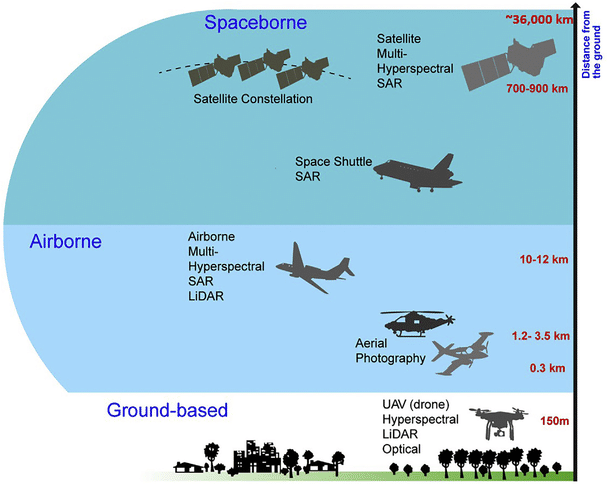
\includegraphics[width=0.7\textwidth]{Immagini/Generiche/Common-Remote-Sensing-Platform-a.png}
    \caption{Rappresentazione delle piattaforme \cite{Rappresentazione_piattaforme}.}
    \label{fig:Classificazione_Piattaforme}
    %Figura 2.1: Esempio schematico di un neurone
\end{figure}



    \newpage
\section{Acquisizione delle informazioni nel telerilevamento}
\subsection{Le Radiazioni elettromagnetiche}
L'acquisizione delle informazioni da remoto su un territorio è possibile attraverso 
l'uso di radiazioni elettromagnetiche (EMR) \cite{OndeEletroMagnetiche}, che vengono emesse o riflesse 
dagli oggetti osservati.
Una radiazione elettromagnetica è una perturbazione di natura simultaneamente 
elettrica e magnetica che si propaga nello spazio e che può trasportare energia.  

% Essa è  lunghezza d’onda 
% $(\lambda)$, frequenza $(f)$ e ampiezza $(A)$. 
% La lunghezza d’onda è la distanza che separa due creste consecutive; la frequenza equivale al numero di picchi
% d’onda che passano in un punto in un intervallo di tempo di un secondo, ed è inversamente
% proporzionale alla lunghezza d’onda; l’ampiezza è la distanza del massimo della cresta dall’asse di
% propagazione dell’onda.

\begin{figure}[H]
    \centering
    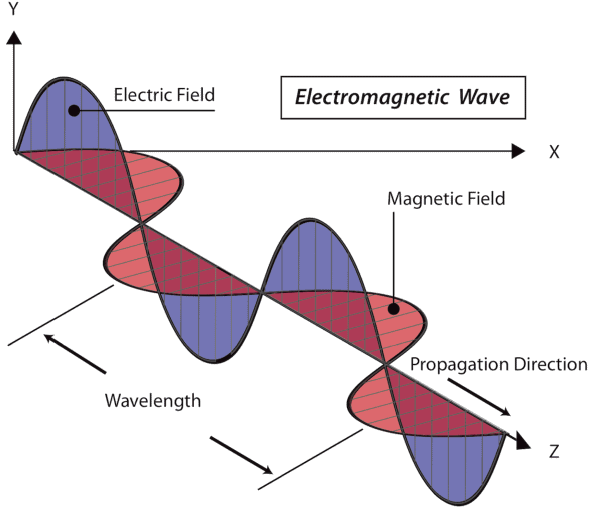
\includegraphics[width=0.44\textwidth]{Immagini/Generiche/OndaElettromagnetica.png}
    \caption{Rappresentazione dell’onda elettromagnetica \cite{Onda_IMG}.}
    \label{fig:onda_elettromagnetica}
\end{figure}

Un’onda elettromagnetica è caratterizzata da tre parametri fondamentali :

\begin{itemize}
    \item \textbf{Lunghezza d’onda $(\lambda)$} la quale esprime la distanza tra due creste d’onda 
    consecutive. La lunghezza d’onda si misura in metri [$m$], o in sottomultipli 
    del metro, come i nanometri ($nm$, $10^{-9}$ metri) o i micrometri ($\mu m$, $10^{-6}$ 
    metri); 

    \item \textbf{Frequenza $(f)$}, cioè il numero dei picchi d’onda che passano in un punto in 
    un certo intervallo di tempo $t$; la frequenza è di solito misurata in hertz [$\text{Hz}$], 
    che è equivalente ad un ciclo al secondo;

    \item \textbf{Ampiezza A}, che è l’altezza di ogni picco d’onda.
\end{itemize}

La frequenza e la lunghezza d’onda sono legate da una relazione, che è definita come:
\begin{equation}
    \lambda = \frac{C}{f}
\end{equation}

dove $C$ è una costante che ha valore $\textit{299.792.458}\ m/s$. Questa costante 
è la velocità della luce e rappresenta la velocità con cui si propaga 
l'onda elettromagnetica attraverso lo spazio. 

\newpage
\subsection{Lo Spettro Elettromagnetico}
La figura (\ref{fig:BandeSpettroElettromagnetico}) rappresenta lo spettro
elettromagnetico (o spettro EM), una distribuzione monodimensionale 
continua dell’energia elettromagnetica, ordinata per lunghezze d’onda $(\lambda)$ crescenti.  
In pratica, lo spettro elettromagnetico è l’insieme di tutte le possibili 
frequenze delle onde elettromagnetiche \cite{spetto_magnetico}.

\begin{figure}[H]
    \centering
    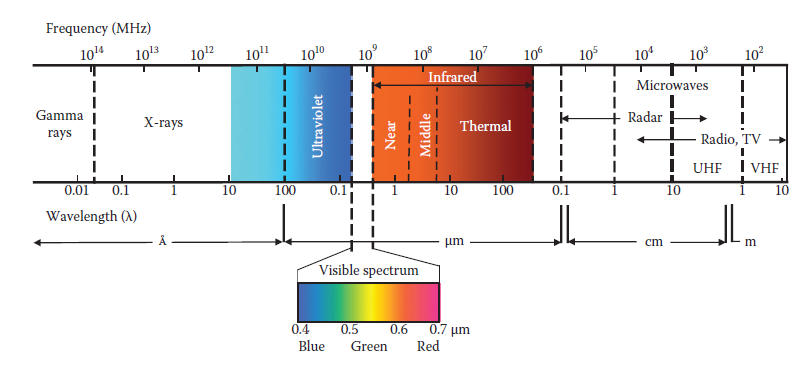
\includegraphics[width=0.95\textwidth]{Immagini/Generiche/BandeSpettroElettromagnetico.png}
    \caption{Bande dello spettro elettromagnetico \cite{SPETTRO_IMG} .}
    \label{fig:BandeSpettroElettromagnetico}
\end{figure}

Come si può osservare, lo spettro è diviso in sette intervalli (anche detti bande),
ciascuna della quali racchiude un insieme di frequenze (o lunghezze d’onda) 
appartenenti alla stessa tipologia di radiazione.

% \begin{figure}[H]
%     \centering
%     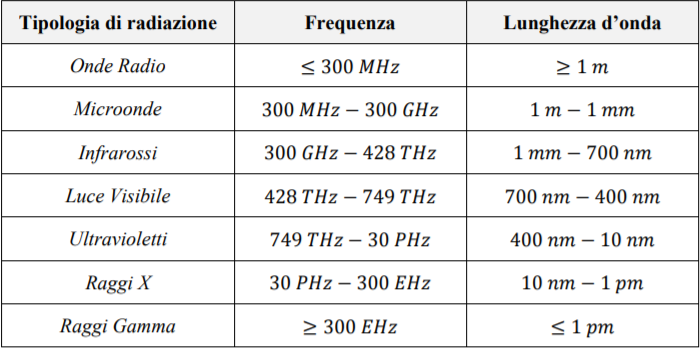
\includegraphics[width=0.65\textwidth]{Immagini/Generiche/Tabella_frequenze.png}
%     \caption{ Classificazione delle radiazioni elettromagnetiche.}
%     \label{fig:Classificazion_radiazioni_elettromagnetiche.}
% \end{figure}

\begin{table}[H]
    \centering
    \begin{tabular}{|p{5cm}|p{5cm}|p{5cm}|}
        \hline
        \textbf{Tipologia di radiazione} & \textbf{Frequenza} & \textbf{Lunghezza d’onda} \\
        \hline
        \textit{Onde Radio} & $\leq 300$ MHz & $\geq 1$ m \\
        \hline
        \textit{Microonde} & $300$ MHz – $300$ GHz & $1$ m – $1$ mm \\
        \hline
        \textit{Infrarossi} & $300$ GHz – $428$ THz & $1$ mm – $700$ nm \\
        \hline
        \textit{Luce Visibile} & $428$ THz – $749$ THz & $700$ nm – $400$ nm \\
        \hline
        \textit{Ultravioletti} & $749$ THz – $30$ PHz & $400$ nm – $10$ nm \\
        \hline
        \textit{Raggi X} & $30$ PHz – $300$ EHz & $10$ nm – $1$ pm \\
        \hline
        \textit{Raggi Gamma} & $\geq 300$ EHz & $\leq 1$ pm \\
        \hline
    \end{tabular}
    \caption{Tabella riassuntiva delle frequenze di ogni tipologia di radiazione.}
\end{table}

Lo spettro del visibile (visible spectrum) è quella parte dello spettro 
elettromagnetico, compresa tra i $400\ nm$ (viola) e $700\ nm$ (rosso), che è percepibile 
all’occhio umano.
% È importante notare come questa sia l’unica parte dello spettro a cui sia 
% possibile associare il concetto di colore.

Tra le diverse regioni spettrali, quelle che vengono principalmente utilizzate 
per l'acquisizione di informazioni su un territorio sono: l'infrarosso (Infrared), 
il visibile (visible) e l'ultravioletto (Ultraviolet). 

% \subsection{Interazioni con l’atmosfera e con la superficie terrestre}
% % La radiazione solare, prima di raggiungere la superficie terrestre percorre 
% % l’atmosfera: in questo passaggio una parte dell’energia è riflessa verso l’alto; 
% % un’altra parte viene invece assorbita e poi riemessa in tutte le direzioni come 
% % radiazione termica; una parte viene diffusa. L’energia elettromagnetica riflessa e 
% % parte di quella diffusa trasporta le informazioni registrate dai radiometri e dai 
% % sensori utilizzati nel telerilevamento.

% Le radiazioni elettromagnetiche posso interagire in diversi 
% modi con l’atmosfera e con la superficie terrestre. 
% Tali interazioni possono essere rilevanti o trascurabili ai fini dei rilievi spettrali, in
% quanto, a seconda del percorso che l’onda deve percorrere prima di essere catturata dal sensore,
% possono influenzare la misurazione del sensore.

% % Le interazioni atmosferiche della radiazione elettromagnetica possono essere 
% % rilevanti o trascurabili ai fini dei rilievi spettrali, a seconda del percorso che l’onda 
% % deve percorrere prima di essere catturata dal sensore. Maggiore è tale percorso, 
% % maggiori sono le influenze atmosferiche sulla radianza registrata dal sensore: se il 
% % sensore è montato su un aereo che vola a bassa quota o se le misure vengono 
% % effettuate a terra, gli effetti dell’atmosfera nella radiazione riflessa sono minimi; al 
% % contrario i sensori montati su satellite ne sono molto influenzati, perché la 
% % radiazione riflessa deve attraversarla completamente prima di raggiungerli.


% L’atmosfera modifica la radiazione in tre modi differenti:
% \begin{itemize}
%     \item Diffusione;
%     \item Assorbimento atmosferico;
%     \item Rifrazione.
% \end{itemize}

% Mentre la superficie terrestre interagisce con la radiazione elettromagnetica
% attraverso processi di:

% \begin{itemize}
%     \item Riflessione;
%     \item Trasmissione;
%     \item Assorbimento terrestre.
% \end{itemize}

% La figura (\ref{fig:interazioni_ondeElettromagnetiche}) mostra un rappresentazione 
% di queste interazioni:

% \begin{figure}[H]
%     \centering
%     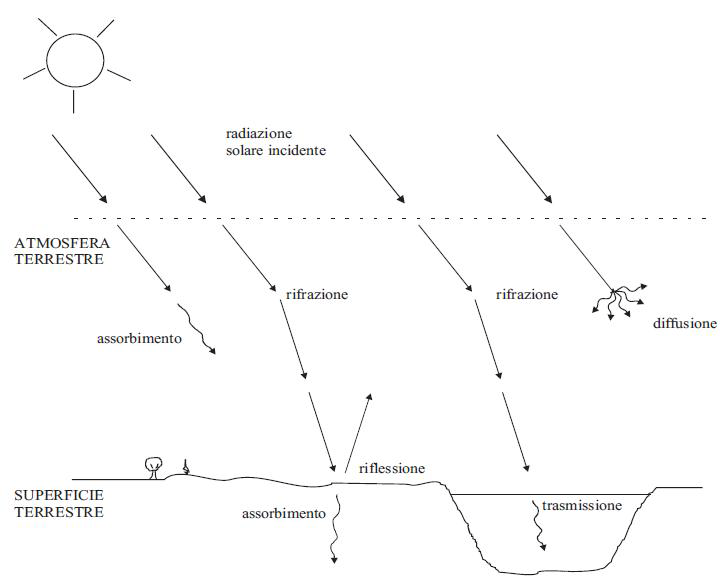
\includegraphics[width=0.70\textwidth]{Immagini/Generiche/interazioni_ondeElettromagnetiche.png}
%     \caption{Interazioni con le onde elettromagnetiche \cite{INTERAZIONI_ONDE}}
%     \label{fig:interazioni_ondeElettromagnetiche}
%     %Figura 2.1: Esempio schematico di un neurone
% \end{figure}

% La \textbf{diffusione} si verifica per interazione con le particelle fini o gassose 
% dell’atmosfera e distribuisce in tutte le direzioni la radiazione intercettata. La 
% diffusione avviene in prevalenza per le radiazioni a lunghezza d’onda più bassa, 
% vale a dire per quelle nel campo del violetto e del blu.

% La \textbf{rifrazione} avviene quando il fascio di luce attraversa due mezzi differenti 
% in grado di trasmettere la radiazione. Nell’atmosfera questo fenomeno avviene al 
% passaggio dei diversi strati atmosferici caratterizzati da umidità e temperature 
% differenti. Tali variazioni influenzano la densità degli strati atmosferici causando 
% una curvatura del raggio che li attraversa. Questo fenomeno è osservabile d’estate
% quando è percepibile un tremolio degli oggetti posti a distanza, dovuto al 
% passaggio della luce vicino a superfici molto calde, come ad esempio il manto 
% stradale. 

% L’\textbf{assorbimento atmosferico} si verifica per l’interazione della radiazione 
% elettromagnetica con i gas presenti nell’atmosfera, quali ozono, ossigeno, anidride 
% carbonica e vapor acqueo. Questi gas assorbono l’energia contenuta nella 
% radiazione luminosa per poi riemetterla sotto forma di energia radiante con 
% lunghezza d’onda maggiore.

% La \textbf{riflessione} avviene quando un raggio luminoso incide su una superficie non 
% trasparente e viene diretto in un’altra direzione. Il tipo di riflessione dipende dalle 
% dimensioni delle irregolarità della superficie: se essa è liscia in 
% relazione alla lunghezza d’onda, si verifica il fenomeno della riflessione speculare 
% in cui tutta la radiazione incidente viene riflessa in un'unica direzione, se la 
% superficie è invece irregolare si comporta come un riflettore isotropo (o diffuso) e 
% la luce viene riflessa in modo diffuso. 

% La \textbf{trasmissione} avviene quando la radiazione passa attraverso un mezzo senza 
% subire una significativa attenuazione.

% L’\textbf{assorbimento terrestre} della radiazione elettromagnetica può avvenire in 
% base alle caratteristiche chimico-fisiche dei corpi che vi si trovano. Ad esempio la 
% vegetazione assorbe gran parte della radiazione incidente della banda del rosso, 
% per poi riemetterla sotto forma di energia termica a lunghezza d’onda maggiore. In 
% natura ogni oggetto ha un comportamento spettrale caratteristico 
% \cite{fenomeni_luce,fenomeni_luce_2,ALL1_REMOTE_SENSING,ALL6_REMOTE_SENSING}. 

\newpage
\subsection{La Radianza e la Riflettanza}
Nel telerilevamento, quello che viene misurato dai sensori è la Radianza e Riflettanza. 
La radianza è definita come la quantità di radiazione elettromagnetica riflessa 
(o trasmessa) per unità di superficie e di angolo solido (angolo nello spazio 
tridimensionale). La radianza rappresenta una grandezza fondamentale nel 
telerilevamento in quanto molto utile per quantificare la luce riflessa da un 
oggetto che viene ricevuta da un sensore rivolto verso di essa. Questa grandezza 
fisica è legata sia alla geometria dell’osservazione, sia alle caratteristiche del 
sensore e permette di descrivere come la radiazione si distribuisce nello spazio
\cite{Radianza, ALL6_REMOTE_SENSING}. 

La radianza è caratterizzata dalla seguente formula: 
\begin{equation}
    L = \frac{P}{A \Omega \cos ({\theta})} \left[\frac{W}{m^2sr}\right]
\end{equation}

dove:
\begin{itemize}
    \item $L$ è la radianza;
    \item $P$ è la potenza in watt;
    \item $\theta$ è l'angolo compreso tra la normale alla superficie e la direzione specificata;
    \item $A$ è la superficie emittente;
    \item $\Omega$ è l'angolo solido.
\end{itemize}

\begin{figure}[H]
    \centering
    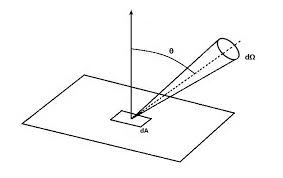
\includegraphics[width=0.40\textwidth]{Immagini/Grafici/radianza.png}
    \caption{Rappresentazione della radianza \cite{RADIANZA_IMG}.}
    \label{fig:Radianza}
    %Figura 2.1: Esempio schematico di un neurone
\end{figure}

La riflettanza invece è il rapporto tra la quantità di radiazione emessa (ovvero 
che colpisce una superficie) e la quantità di radiazione riflessa (o ricevuta) dalla stessa 
ed è quindi un numero puro generalmente minore di uno. 
Questa grandezza è indispensabile per l’individuazione e la discriminazione dei 
campioni oggetto di analisi, in quanto consente di svincolarsi completamente da 
condizioni variabili nel tempo (che influenzano la radianza) al momento 
dell’acquisizione, rendendo confrontabili misure condotte in momenti diversi
\cite{Riflettanza, ALL6_REMOTE_SENSING}. 
La riflettanza può essere espressa come: 

\begin{equation}
    \rho = \frac{\Phi_r}{\Phi_0}
\end{equation}

dove:
\begin{itemize}
    \item $\rho$ è la riflettanza;
    \item $\Phi_r$ il flusso luminoso riflesso;
    \item $\Phi_0$ il flusso luminoso incidente;
\end{itemize}
Ciò che viene direttamente misurato dal sensore è la radianza, per questo è necessaria una corretta 
calibrazione del sensore al fine di ottenere dati confrontabili.



\subsection{Firma spettrale}
Quando la riflettanza o la radianza è calcolata su tutte le frequenze dello spettro, 
si parla allora di \textbf{firma spettrale}. 

%L'imaging multispettrale si basa sulla spettroscopia e sull'ottica.
Ogni oggetto o unità di territorio (roccia, vegetazione…) ha la propria \textbf{firma spettrale} (o impronta digitale spettrale), 
che specifica il modo in cui le lunghezze d'onda della luce vengono assorbite, riflesse o trasmesse attraverso 
quell'oggetto \cite{Firma_spettare}. %Tale proprietà determina il colore nel campo visibile.
% Per esempio, confrontando la firma spettrale di campioni sconosciuti 
% con quella di sostanze note, è possibile identificata la composizione chimica del 
% campione ignoto.

\begin{figure}[H]
    \centering
    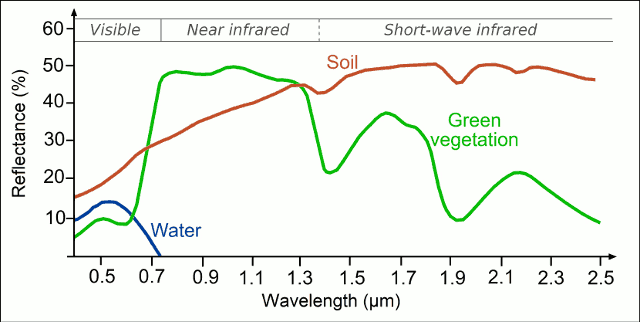
\includegraphics[width=0.70\textwidth]{Immagini/Generiche/spectral_sign.png}
    \caption{Esempi di firme spettrali per acqua, suolo, vegetazione \cite{ALL2_REMOTE_SENSING}.}
    %Figura 2.1: Esempio schematico di un neurone
\end{figure}

Ad esempio i canali utilizzati per la copertura della vegetazione catturano 
l'intensità della luce dal visibile all'infrarosso, consentendo di valutare l'attività fotosintetica e lo stato 
delle piante. I canali per il monitoraggio delle superfici terrestri possono registrare 
l'energia in una gamma più ampia, che comprende gli ultravioletti e le microonde.

\section{Tipologie di sensori}
I sensori possono essere classificati in base a diversi fattori.
Una delle classificazioni più comuni vede i sensori suddivisi in due gruppi: sensori passivi e 
sensori attivi. 
\begin{itemize}
    \item I \textbf{sensori passivi} si limitano a misurare la radiazione elettromagnetica derivata da 
    fonti esterne: ad esempio, l’energia della radiazione solare riflessa dalla superficie 
    terrestre o l’energia direttamente emanata dalla Terra, ovvero la Radianza. 
    Questi sensori sono stati ampiamente utilizzati nel telerilevamento negli ultimi decenni e includono: 
    fotocamere, scanner elettro-ottici e radiometri a microonde.

    \begin{figure}[H]
        \centering
        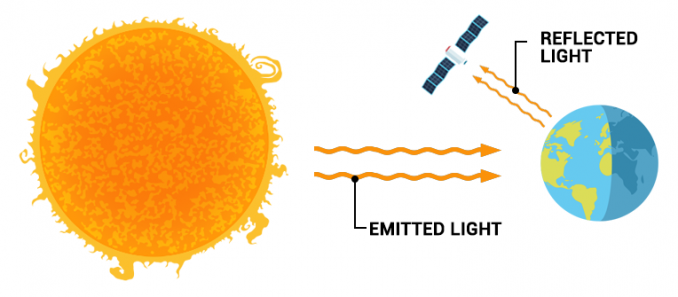
\includegraphics[width=0.65\textwidth]{Immagini/Generiche/Passive-Remote-Sensing.png}
        \caption{Illustrazione funzionamento sensori passivi \cite{GISGeography_RemoteSensing}}
        %Figura 2.1: Esempio schematico di un neurone
    \end{figure}

    \item I \textbf{sensori attivi} sono invece quelli che misurano la radiazione emessa da una fonte 
    di energia incorporata nello strumento stesso e che viene riflessa dalle superfici 
    inquadrate. Ovvero che si basano sul concetto della riflettanza. Questi sono in grado di inviare impulsi e registrare in seguito la loro 
    riflessione per caratterizzare gli oggetti. Queste tipologie di sensori
    sono ad esempio radar o LiDAR.

    \begin{figure}[H]
        \centering
        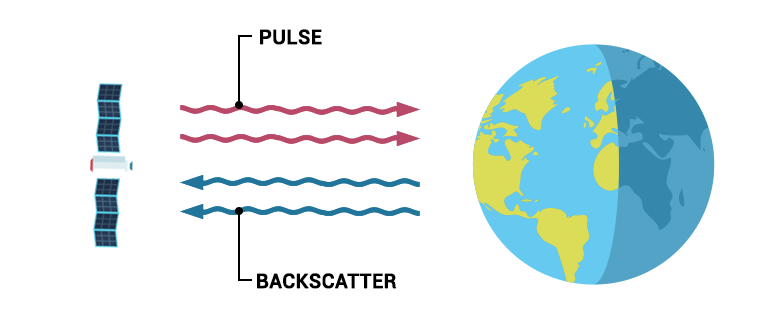
\includegraphics[width=0.65\textwidth]{Immagini/Generiche/Active-Remote-Sensing.png}
        \caption{Illustrazione funzionamento sensori attivi \cite{GISGeography_RemoteSensing}}
        %Figura 2.1: Esempio schematico di un neurone
    \end{figure}

\end{itemize}

I sensori posso essere classificati anche in base al numero di bande che sono in grado di acquisire, i sensori possono essere 
multispettrali o iperspettrali. 

\begin{itemize}
    \item I \textbf{sensori multispettrali} di solito riescono ad acquisire 
    da 3 a 10 bande circa. Le bande che vengono normalmente acquisite sono quelle 
    del visibile, rosso, verde, blu, e quella del vicino infrarosso.

    \item I \textbf{sensori iperspettrali}, invece, misurano l'energia in bande più strette e numerose rispetto ai sensori 
    multispettrali. Le immagini iperspettrali, infatti, possono contenere fino a 200 (o 
    più) bande spettrali. 
\end{itemize}
    
\section{Immagini Multispettrali e Iperspettrali}
Nelle immagini multispettrali, così come in quelle iperspettrali, ogni pixel 
dell’immagine non è costituito da un solo valore monocromatico, 
come nel caso delle immagini pancromatiche (a scala di grigi), o da una terna di valori, 
come nel caso delle immagini a colori RGB, ma da un insieme di valori appartenenti 
allo spettro elettromagnetico. 
Nella scienza del processamento delle immagini, questi valori sono
anche noti come \textbf{Canale} \cite{ALL6_REMOTE_SENSING,immagini_multispettrali2,immagini_multispettrale3,ALL2_REMOTE_SENSING}.

A differenza delle immagini multispettrali, le iperspettrali possiedono un numero elevato di bande, 
che rappresentano intervalli discreti dello spettro elettromagnetico, e producono uno spettro 
continuo per ogni pixel ritratto nella scena. Tipicamente, un'immagine multispettrale
possiede un numero di canali che varia dai 3 fino ad arrivare a 13. In alcuni casi si 
utilizzano anche 15 canali.
Mentre nelle immagini iperspettrali, il numero di canali si aggira intorno alle centinaia:
tipicamente si utilizzano 100 o 200 canali, ma è possibile arrivare anche a numeri ben 
più elevati
\cite{Immagini_multispettrali,immagini_multispettrali2,immagini_multispettrale3,ALL2_REMOTE_SENSING}.
\newpage
La figura (\ref{fig:Multy_vs_Hyper_spectral}) mette in risalto la differenza 
tra queste due tipologie di immagini.

\begin{figure}[H]
    \centering
    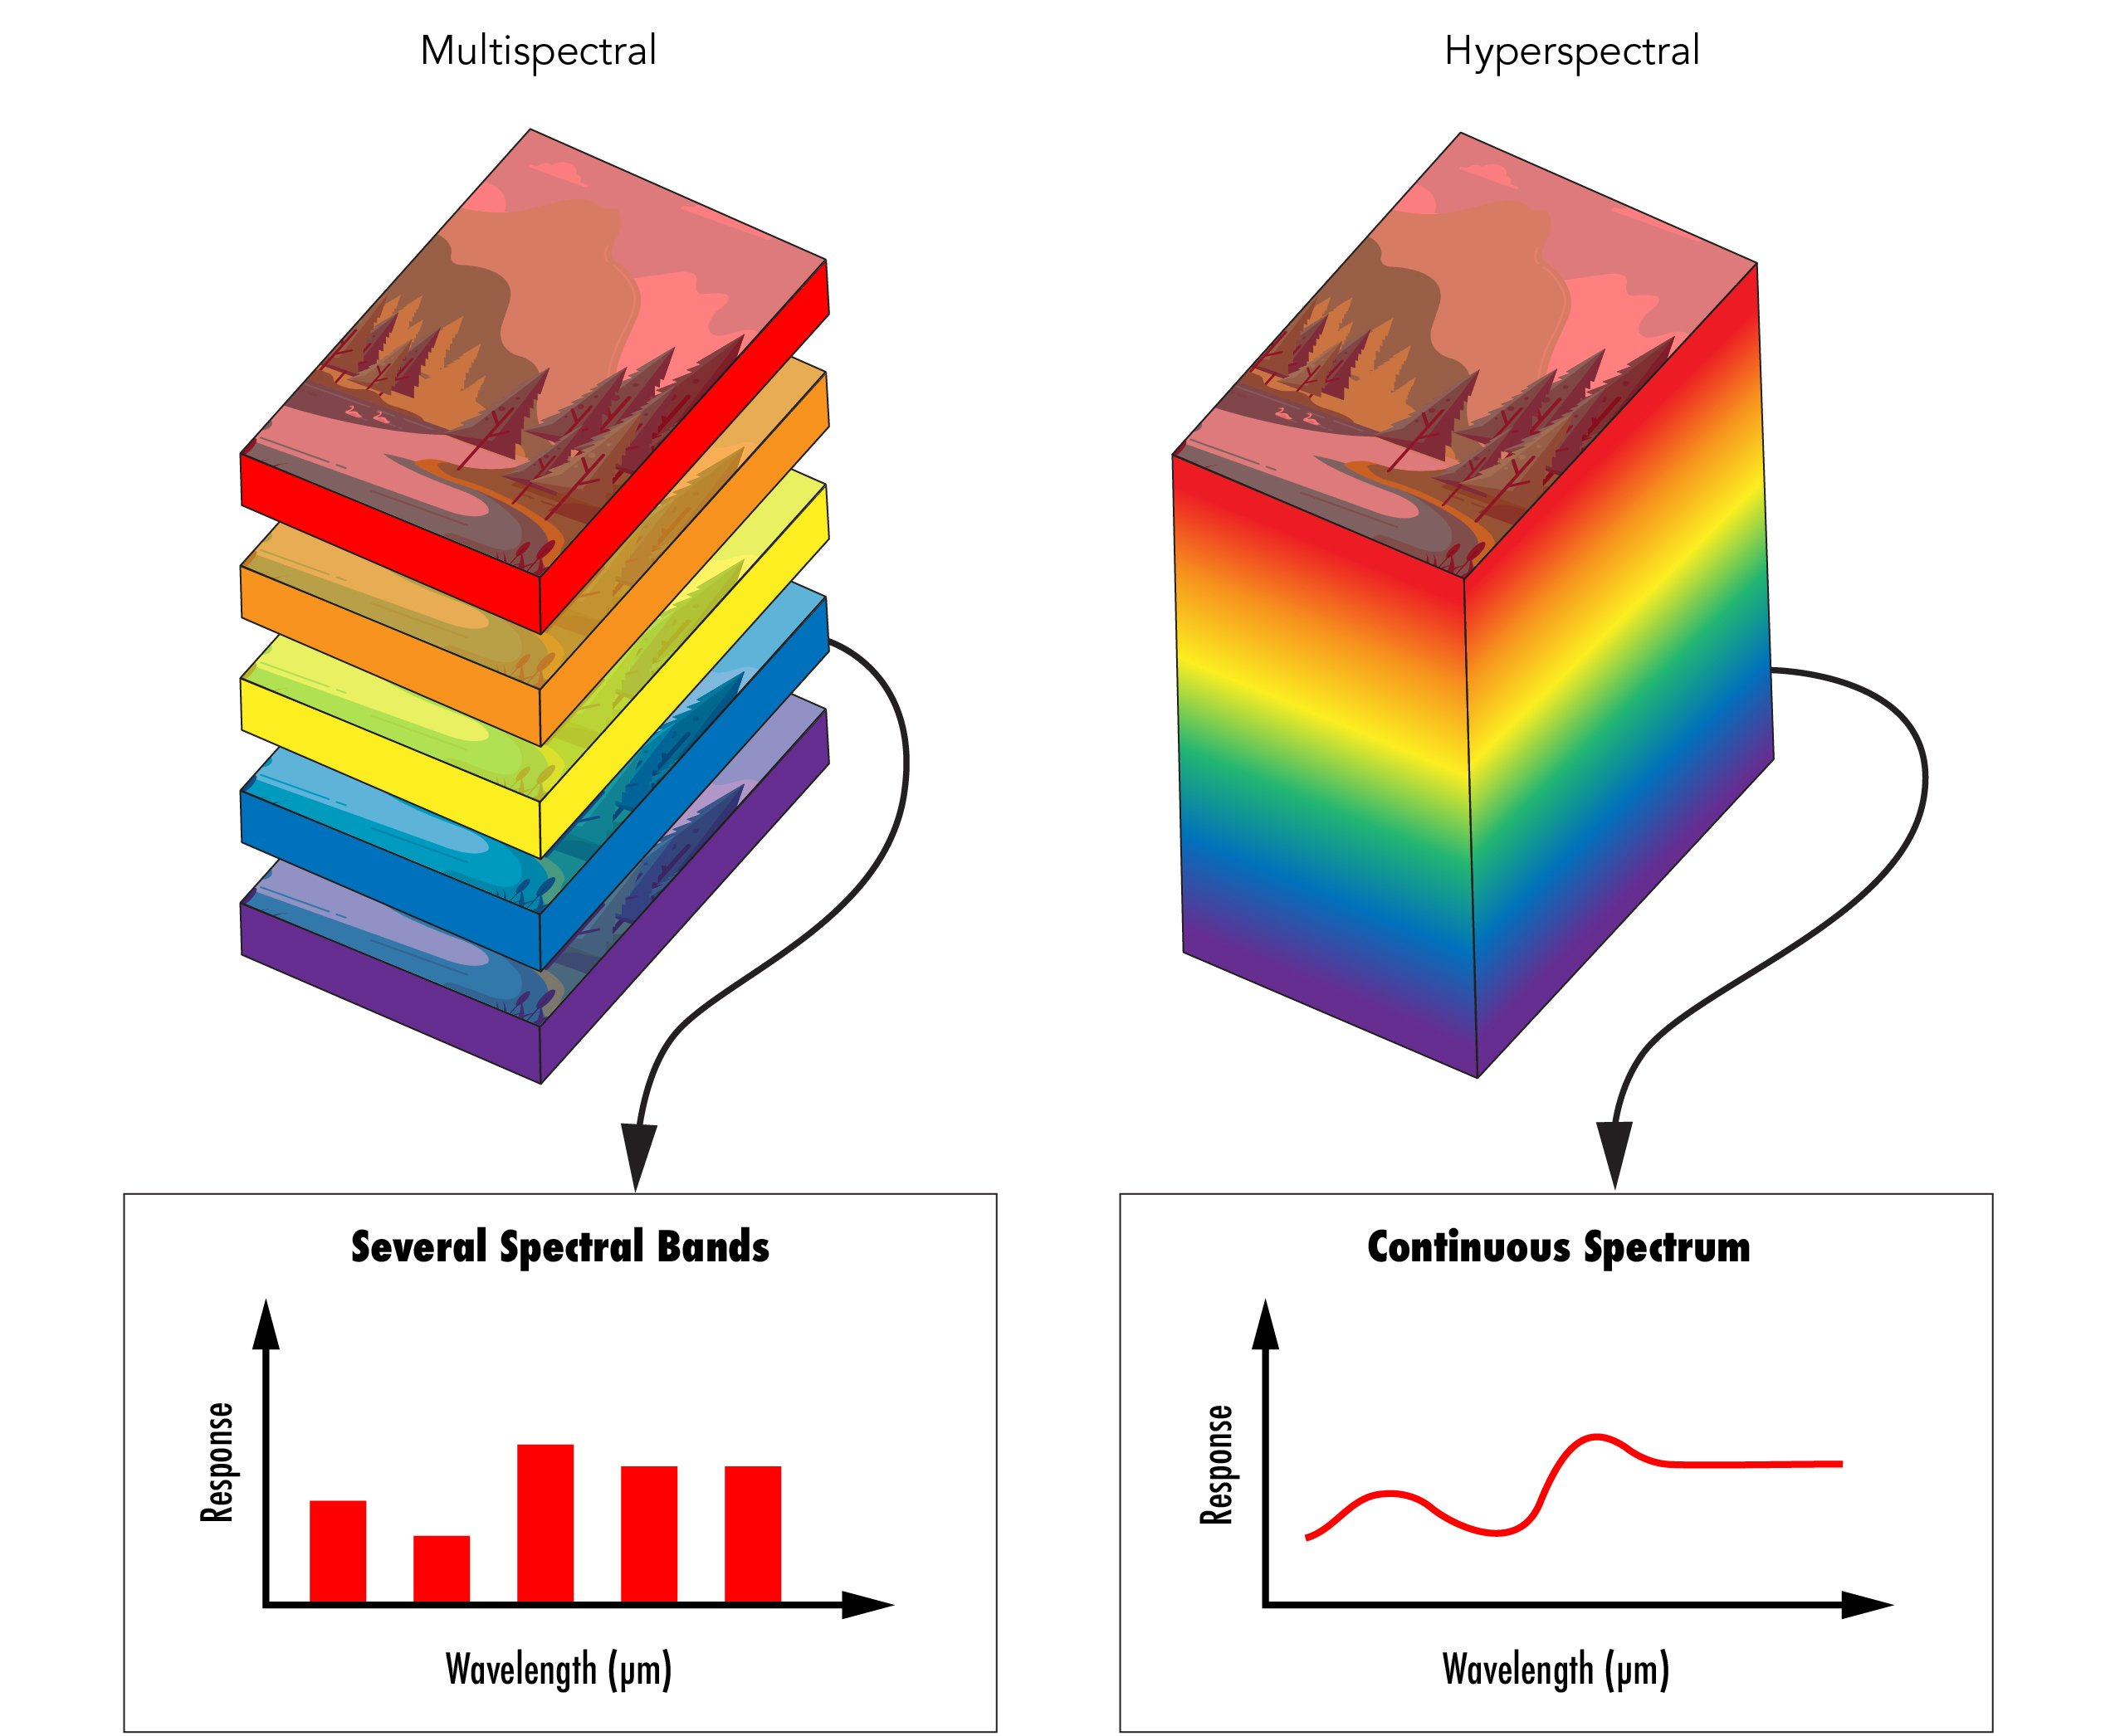
\includegraphics[width=0.60\textwidth]{Immagini/Generiche/Multy_vs_Hyper_spectral.png}
    \caption{ Confronto tra Multispectral e Hyperspectral Imaging \cite{Immagini_multispettrali}.}
    \label{fig:Multy_vs_Hyper_spectral}
    %Figura 2.1: Esempio schematico di un neurone
\end{figure}

Come si può osservare dalla figura \ref{fig:Multy_vs_Hyper_spectral}, 
una singola immagine iperspettrale o multispettrale può essere vista come un 
cubo di dati, in cui le informazioni spaziali sono disposte lungo l'asse X e 
l'asse Y, mentre le informazioni di carattere spettare sono disposte 
lungo l'asse Z \cite{Immagini_multispettrali}.
% Una singola immagine iperspettrale/multispettrale può essere considerata come un 
% cubo di dati, in cui le informazioni spaziali sono raccolte sul piano X-Y, 
% mentre le informazioni spettrali sono rappresentate lungo l’asse Z. 
% Lungo quest’ultima direzione il cubo è costituito da tanti piani quante sono le bande 
% che compongono lo spettro telerilevato.
 

\begin{figure}[H]
    \centering
    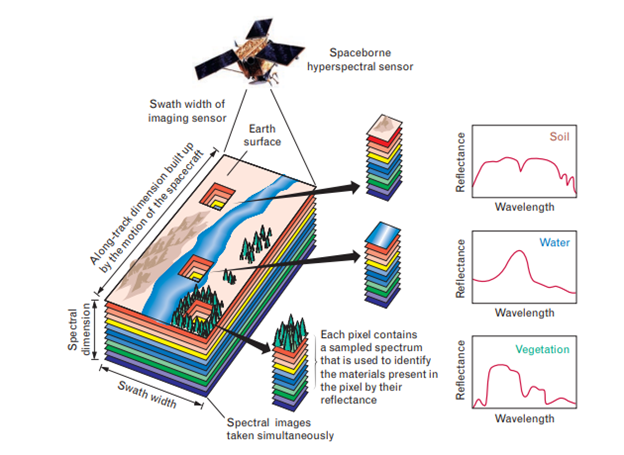
\includegraphics[width=0.80\textwidth]{Immagini/Generiche/scansionamento_terreno.png}
    \caption{Rappresentazione grafica dell'acquisizione di dati \cite{immagini_multispettrali2} .}
    \label{fig:bho1}
    %Figura 2.1: Esempio schematico di un neurone
\end{figure}

% Spesso lo spettro associato ad un pixel è uno spettro di riflettanza, 
% che può contenere fino a centinaia di valori monocromatici. La riflettanza è una 
% grandezza adimensionale, compresa tra 0 e 1, che rappresenta l’efficienza con la 
% quale una superficie riesce a riflettere la luce di una data lunghezza d’onda.

L'utilizzo di diversi canali spettrali fornisce informazioni più complete e accurate 
sulla superficie terrestre. Ogni canale registra informazioni sulla luce in una gamma 
specifica di lunghezze d'onda, che possono essere utili per applicazioni e compiti 
specifici.




 










\subsection{Visualizzazione delle diverse bande}

Le immagini a colori sono composte da 3 canali: il rosso, verde e il blu. Questi canali
vengono sovrapposti per permettere la visualizzazione a colori reali dell'immagine.

\begin{figure}[H]
    \centering
    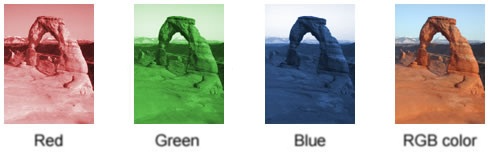
\includegraphics[width=0.60\textwidth]{Immagini/Generiche/canali_rgb.png}
    \caption{Rappresentazione di un immagine a colori.}
    %\label{fig:Classificazion_radiazioni_elettromagnetiche}
\end{figure}

Quando abbiamo un'immagine composta da diverse bande (come le immagini multispettrali e 
iperspettrali), la cosa più semplice (ma in genere meno interessante) che possiamo fare 
è visualizzare singolarmente ogni banda in scala di grigi oppure utilizzare delle heatmap. 

Se vogliamo un'immagine a colori dobbiamo scegliere tre bande a cui assegnare i tre 
colori fondamentali R (Red), G (Green), B (Blue). Se usiamo le bande che corrispondono 
effettivamente a rosso, verde e blu otteniamo un'immagine in colori reali, se invece 
usiamo anche le altre bande avremo un'immagine in falsi colori \cite{immagini_multispettrali_a_colori}.

\begin{figure}[H]
    \centering
    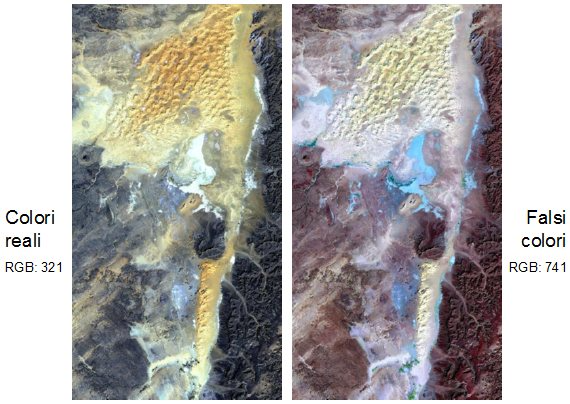
\includegraphics[width=0.75\textwidth]{Immagini/Generiche/paragone_bande.png}
    \caption{Differenze dell'utilizzo di diversi canali \cite{immagini_multispettrali_a_colori} .}
    %\label{fig:Classificazion_radiazioni_elettromagnetiche}
\end{figure}

La combinazione delle diverse bande dipende da cosa vogliamo visualizzare e 
mettere in risalto.
    \newpage
\section{Copernicus e Sentinel-2}
\subsection{Il programma spaziale Europeo Copernicus}
Copernicus \cite{COPERNICUS_INFO} è il nome dell’innovativo programma di 
monitoraggio del pianeta Terra portato avanti dall’Unione Europea.
Il programma è coordinato e gestito dalla Commissione europea ed è attuato in 
collaborazione con gli Stati membri, l'Agenzia spaziale europea (ESA), 
l'Organizzazione europea per l'esercizio dei satelliti meteorologici (EUMETSAT), 
il centro europeo per le previsioni meteorologiche a medio termine (CEPMMT), 
le agenzie dell'UE e il Mercator Océan.
Il programma Copernicus, iniziato nel 2014, si propone di fornire 
informazioni di libero accesso in merito alle condizioni del pianeta, 
al fine di informare e aiutare nelle decisioni le autorità, i cittadini, i 
ricercatori e le organizzazioni. Questo per offrire servizi in sei 
campi: atmosfera, ambiente marino, 
territorio, cambiamenti climatici, sicurezza ed emergenze. 
Il programma Copernicus è costituito da un insieme di satelliti in orbita 
e da altri sistemi aerei, terrestri o marittimi (detti in situ, ovvero non spaziali), 
i quali generano enormi quantità di dati su misurazioni e fotografie del pianeta.
Questi dati vengono poi resi disponibili al pubblico  
in seguito a elaborazioni e archiviazioni.

\subsection{Le missioni Sentinel}

I satelliti principali utilizzati dal programma sono quelli appartenenti 
alla classe \textit{Sentinel} (Sentinelle), i quali sono stati progettati e 
lanciati dall'Agenzia Spaziale Europea (ESA) appositamente per il programma 
Copernicus. Vengono utilizzati 
anche satelliti preesistenti o commerciali per dati complementari (in questo caso si parla 
di missioni partecipanti). Il programma ha attualmente attive 6 missioni Sentinel, ognuna delle 
quali è basata su una costellazione di 2 satelliti: questi ultimi viaggiano sulla stessa orbita 
però sfasati di 180° tra di loro, in modo da garantire tempi di rivisitazione 
(passaggio sopra lo stesso punto della Terra) ottimali. 
Questi satelliti trasportano sensori ottici, radar e strumenti di imaging 
dedicati al monitoraggio delle terre, degli oceani e dell’atmosfera.
I dati sentinel sono accessibili tramite il portale messo a disposizione dall'ESA: 
Sentinel Scientific Data Hub (https://scihub.copernicus.eu/) .

\subsubsection{Sentinel-1}
Sentinel-1 è una missione in orbita quasi-polare \cite{ORBITA_POLARE} (angolo di inclinazione rispetto 
l’equatore pari a 98°) iniziata nel 2014 è costituita dai satelliti Sentinel-1A e Sentinel-1B, 
aventi un sistema radar ad apertura sintetica (che invia e riceve impulsi lateralmente). Lo 
scopo è l’imaging radar della Terra diurno e notturno per il monitoraggio terrestre, 
marittimo e climatico.

% \begin{figure}[H]
%     \centering
%     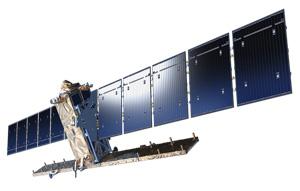
\includegraphics[width=0.3\textwidth]{Immagini/Satelliti/Sentinel_1.png}
%     \caption{Modello di sentinel-1}
% \end{figure}

\subsubsection{Sentinel-2}

Sentinel-2 è una missione in orbita quasi-polare eliosincrona \cite{ELIO_SINCRONA} 
(ovvero sincrona con il sole 
quindi garantisce sempre la stessa luminosità) iniziata nel 2015 è costituita dai satelliti 
Sentinel-2A (lanciato il 23 giugno 2015) e Sentinel-2B (lanciato il 7 marzo 2017). 
Entrambi i satelliti hanno una durata prevista di 7 anni, pertanto saranno 
successivamente sostituiti dai satelliti Sentinel-2C, lanciato il 5 settembre 2024, e 
dal Sentinel-2D.
L’obiettivo è fornire immagini ad alta risoluzione per il 
monitoraggio del territorio, dei cambiamenti climatici, e delle emergenze. 
La copertura garantita dalla missione comprende tutte le terre continentali, comprese
tra le latitudini $56°S$ e $84°N$, i mari fino a $20 km$ dalle coste, tutte le isole europee e
quelle extra-europee con superficie maggiore di $100 km^2$, il Mar Mediterraneo e tutti
i mari chiusi. 

\subsubsection{Sentinel-3}
Sentinel-3 è una missione iniziata nel 2016 costituita dai satelliti Sentinel-3A e Sentinel
3B: monitora la superficie del mare e misura le temperature marine e terrestri, fornendo 
dati ottici, radar e altimetrici. L’obiettivo è il monitoraggio climatico, ambientale e 
oceanografico.

% \begin{figure}[H]
%     \centering
%     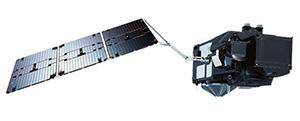
\includegraphics[width=0.3\textwidth]{Immagini/Satelliti/Sentinel_3.png}
%     \caption{Modello di sentinel-3}
% \end{figure}

\subsubsection{Sentinel-4}
Sentinel-4 è una missione non ancora operativa che fornirà dati sulla composizione 
atmosferica (concentrazioni di gas, aerosol e altre componenti).

% \begin{figure}[H]
%     \centering
%     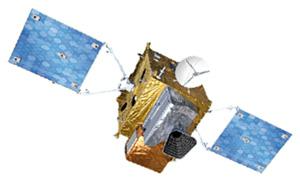
\includegraphics[width=0.3\textwidth]{Immagini/Satelliti/Sentinel_4.png}
%     \caption{Modello di sentinel-4}
% \end{figure}

\subsubsection{Sentinel-5}
Sentinel-5 è una missione non ancora operativa che monitorerà la composizione 
atmosferica: al momento è stato lanciato solo il satellite Sentinel-5P (Precursor) nel 2017, 
che sta rilevando provvisoriamente i dati sulla qualità dell’aria, sul clima e sulle 
radiazioni solari. 

% \begin{multicols}{2}
%     {
%         \begin{figure}[H]
%             \centering
%             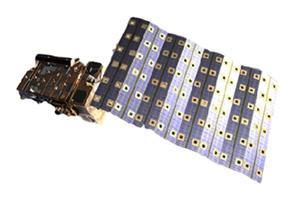
\includegraphics[width=0.25\textwidth]{Immagini/Satelliti/Sentinel_5.png}
%             \caption{Modello di sentinel-5}
%         \end{figure}
%     }
%     {
%         \begin{figure}[H]
%             \centering
%             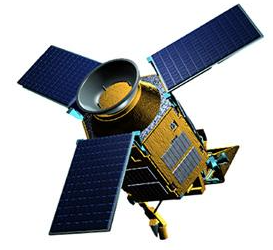
\includegraphics[width=0.25\textwidth]{Immagini/Satelliti/Sentinel_5P.png}
%             \caption{Modello di sentinel-5P}
%         \end{figure}
%     }
% \end{multicols}

\subsubsection{Sentinel-6}
Sentinel-6 è una missione non ancora operativa che misurerà il livello del mare per studi 
su clima e oceanografia. Al momento è stato lanciato solo uno dei satelliti.

% \begin{figure}[H]
%     \centering
%     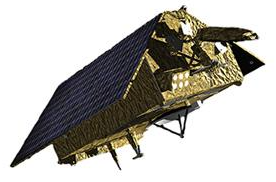
\includegraphics[width=0.3\textwidth]{Immagini/Satelliti/Sentinel_6.png}
%     \caption{Modello di sentinel-6}
% \end{figure}

\subsubsection{Satelliti attualmente in funzione}
I satelliti dedicati attualmente in orbita sono Sentinel-1A e Sentinel-1B, Sentinel-2A e 
Sentinel-2B, Sentinel-3A e Sentinel-3B, Sentinel-5P e Sentinel-6A 


\subsection{Caratteristiche di Sentinel-2}
I satelliti Sentinel-2 viaggiano ad una quota media di 786 km, hanno una swath (area 
analizzata dal satellite) che misura 290 km in larghezza e hanno un frequenza di 
rivisitazione complessiva è elevata (2-5 giorni) \cite{SENTINEL2_2,SENTINEL2_3, ALL_ABOUT_SENTINEL2}.

\begin{figure}[H]
    \centering
    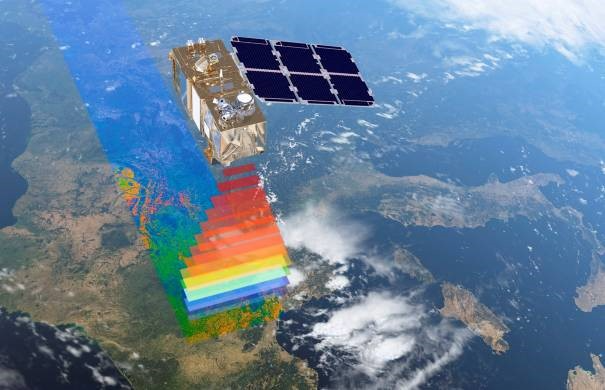
\includegraphics[width=0.5\textwidth]{Immagini/Satelliti/funzionamento_satellite.png}
    \caption{Rappresentazione di un satellite sentinel-2 \cite{immagini_multispettrali2}. }
\end{figure}

I satelliti Sentinel-2 si basano su un sistema di telerilevamento 
passivo, che non emette energia ma registra quella solare riflessa dagli 
oggetti presenti sulla superficie terrestre (a differenza del sistema radar, 
che è attivo quindi invia gli impulsi).

Le immagini prodotte sono multispettrali, perché la quantità di energia riflessa 
viene rilevata dal sensore attraverso diversi intervalli di lunghezze d’onda.
L'acquisizione delle informazioni avviene utilizzato un sistema 
\textit{push-broom}, nel quale due
fila di \textit{detector} (rilevatori), registrano i dati dello swath man mano che il 
satellite procede lungo l’orbita  \cite{ALL_ABOUT_SENTINEL2}. 

\begin{figure}[H]
    \centering
    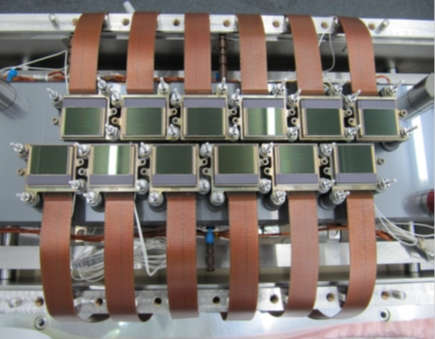
\includegraphics[width=0.3\textwidth]{Immagini/Satelliti/rilevatori_S2.png}
    \caption{Rappresentazione dei rilevatori \cite{ALL_ABOUT_SENTINEL2}.}
\end{figure}

Il rilevatore elettronico utilizzato è di tipo CCD (Charge coupled device) 
ed è costituito da una matrice di pixel, che in base alla quantità di energia 
ricevuta, assegna dei numeri (detti \textit{digital numbers}) ad ogni pixel. 
Questi \textit{digital numbers} (DN) rappresentano la radianza, 
misurata con una risoluzione radiometrica di 12 bit.

I \textit{digital numbers} misurati, vengono poi trasformati in toni di grigio 
per la visualizzazione: ad una maggiore radianza corrisponde un tono più chiaro 
(gli oggetti più chiari riflettono più energia, mentre quelli più scuri 
ne assorbono di più). 
Questo processo permette di generare immagini in bianco e nero per ogni banda spettrale.

La luce riflessa dalla Terra e dalla sua atmosfera verso lo 
MSI (MultiSpectral Instrument) viene raccolta da un telescopio a tre specchi (M1, M2 e M3) e 
focalizzata, tramite un divisore di fascio, su due \textit{Focal Plane Assemblies} (FPA): 
uno per le dieci lunghezze d'onda VNIR e uno per le tre lunghezze d'onda SWIR.
Successivamente i 12 rilevatori, presenti in ogni FPA, registrano la luce incidente, 
convertendola in dati digitali\cite{ALL_ABOUT_SENTINEL2}. 
%Dove ciascuno di questi FPA è composto da 12 rilevatori \cite{ALL_ABOUT_SENTINEL2}. 

\begin{figure}[H]
    \centering
    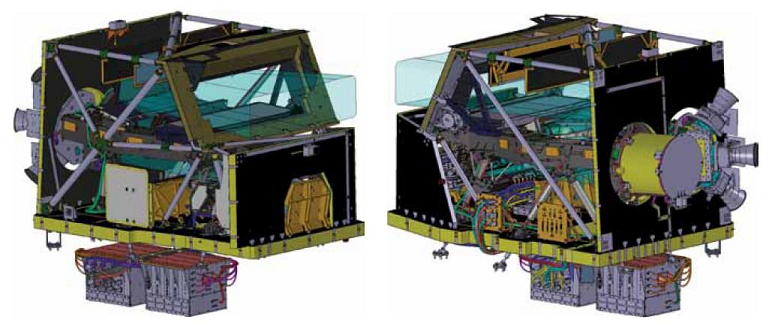
\includegraphics[width=0.5\textwidth]{Immagini/Satelliti/struttura_sentinel2_1.png}
\end{figure}

\begin{figure}[H]
    \centering
    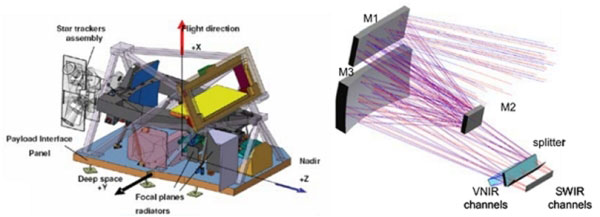
\includegraphics[width=0.7\textwidth]{Immagini/Satelliti/struttura_sentinel2_2.png}
    \caption{Rappresentazione dell'MSI \cite{ALL_ABOUT_SENTINEL2}.}
\end{figure}


Questo permette all'MSI del satellite di acquisire 4 bande nel visibile e 
vicino infrarosso con risoluzione spaziale $10m$, 6 bande nell'infrarosso 
con risoluzione spaziale $20m$ e 3 bande con risoluzione $60m$ di cui una nel 
blu e due nell'infrarosso \cite{MSI_SENTINEL2,ALL_ABOUT_SENTINEL2}.
Per risoluzione spaziale si intende a quale dimensione corrisponde un pixel 
nell'immagine telerilevata, ovvero la distanza coperta da un pixel \cite{ALL3_REMOTE_SENSING}.

\begin{figure}[H]
    \centering
    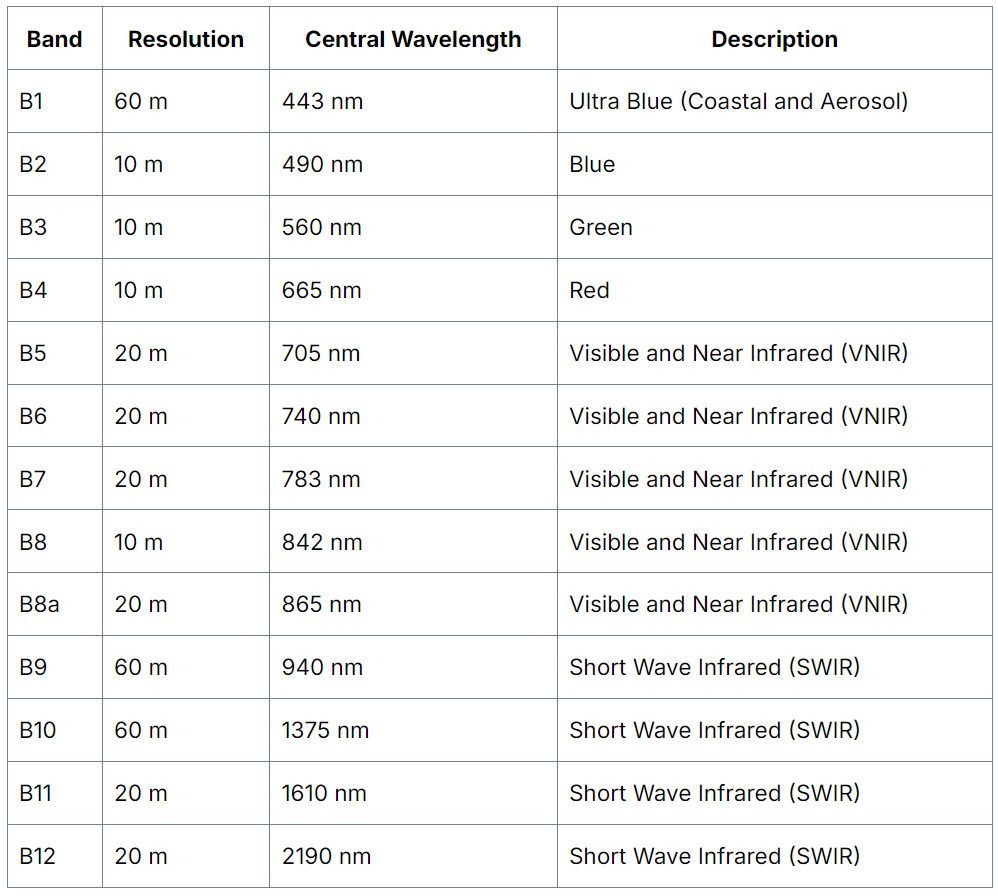
\includegraphics[width=0.70\textwidth]{Immagini/Generiche/Sentinel2_bands_table.png}
    \caption{Caratteristiche delle diverse bande \cite{Tabella_bande, COMBINAZIONE_BANDE_SENTINEL2} .}
    \label{fig:Tabella_bande_s2}
\end{figure}

\subsection{Combinazione delle bande di sentinel-2}
Le diverse bande, oltre a poter essere visualizzate singolarmente in scala di grigi, 
possono essere combinate per mettere in risalto diverse informazioni dell'immagine
\cite{COMBINAZIONE_BANDE_SENTINEL2, SENTINEL2_1_e_bands}.
Alcune delle molte combinazioni che possono essere ottenute utilizzando le bande di 
sentinel-2 sono:

\begin{itemize}
    \item \textbf{Natural Color (B4, B3, B2)}: utilizza i canali 
    rosso (B4), verde (B3) e blu (B2). Il suo scopo è visualizzare le immagini 
    con colori naturali così come la vedrebbero 
    naturalmente gli esseri umani.

    \begin{figure}[H]
        \centering
        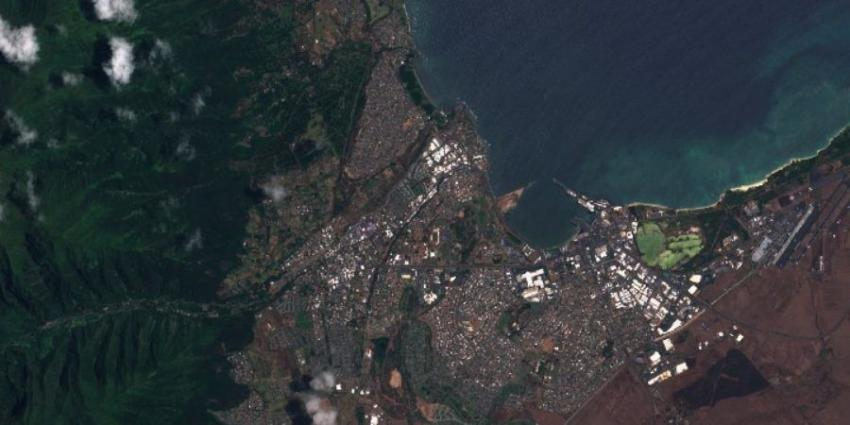
\includegraphics[width=0.6\textwidth]{Immagini/Satelliti/Sentinel-2-Natural-Color-850x425.jpg}
        \caption{Rappresentazione Natural Color.}
    \end{figure}

    \item \textbf{Color Infrared (B8, B4, B3)}: questa combinazione di bande è 
    pensata per enfatizzare la vegetazione sana e non sana. 
    La banda del vicino infrarosso (B8), è particolarmente efficace nel 
    riflettere la clorofilla. Per questo, in un'immagine infrarossa a colori, 
    la vegetazione più densa è rossa. Ma le aree urbane sono bianche.
    
    \begin{figure}[H]
        \centering
        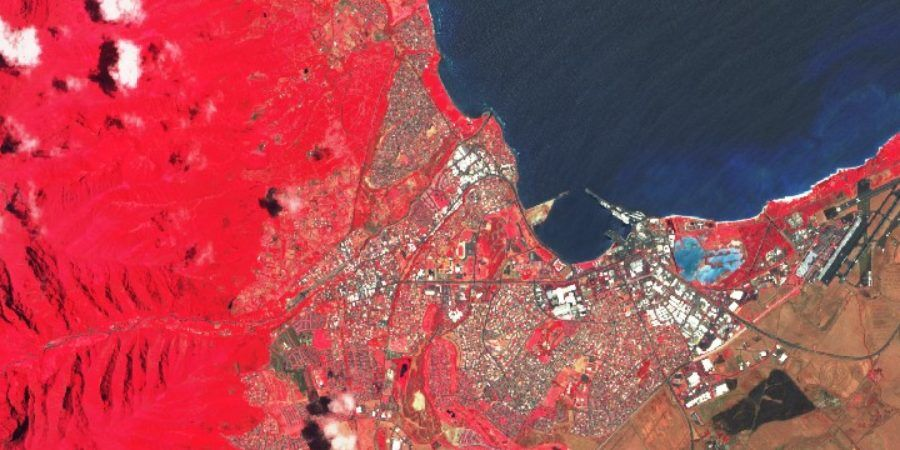
\includegraphics[width=0.6\textwidth]{Immagini/Satelliti/Sentinel-2-Color-Infrared.jpg}
        \caption{Rappresentazione Color Infrared.}
    \end{figure}
    
    \item \textbf{Short-Wave Infrared (B12, B8A, B4)}: utilizza le bande 
    SWIR (B12), NIR (B8A) e Rosso (B4). Questa composizione mostra la vegetazione in 
    varie tonalità di verde. In generale, le tonalità di verde più scure indicano una
    vegetazione più densa. Mentre il marrone può indicare un terreno privo di vegetazione 
    o un'area edificata.
    \begin{figure}[H]
        \centering
        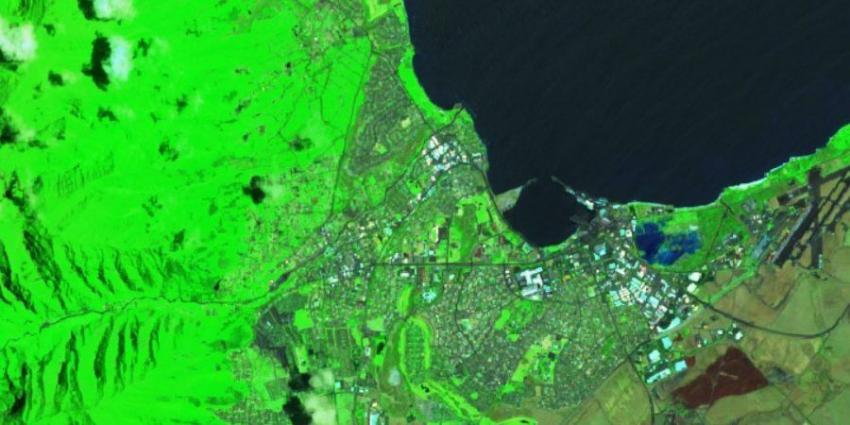
\includegraphics[width=0.6\textwidth]{Immagini/Satelliti/Sentinel-2-Shortwave-Infrared-850x425.jpg}
        \caption{Rappresentazione Short-Wave Infrared.}
    \end{figure}
    
    \newpage
    \item \textbf{Vegetation Index (B8-B4)/(B8+B4)}: Poiché che la 
    vegetazione ha una forte capacità di riflettere la radiazione 
    nel vicino infrarosso (Near Infrared, NIR) e di assorbire quella 
    nella banda del rosso, l'indice di vegetazione è utile per 
    quantificare la quantità di vegetazione presente in un'area. 
    
    \begin{figure}[H]
        \centering
        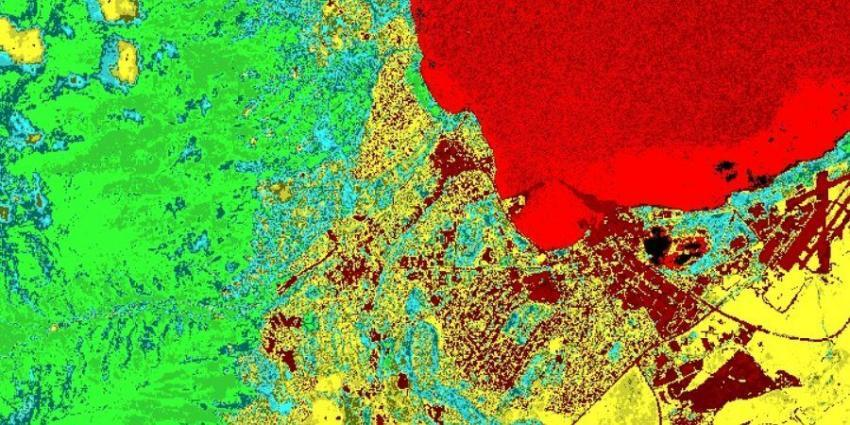
\includegraphics[width=0.6\textwidth]{Immagini/Satelliti/Sentinel-2-Vegetation-Index-850x425.jpg}
        \caption{Rappresentazione Vegetation Index.}
    \end{figure}
    
    \item \textbf{Moisture Index (B8A-B11)/(B8A+B11)}: è ideale per individuare lo 
    stress idrico nelle piante. Utilizza le onde corte e il vicino infrarosso per 
    generare un indice del contenuto di umidità. In generale, la vegetazione più 
    umida ha valori più alti. Ma valori di indice di umidità più bassi suggeriscono 
    che le piante sono sotto stress a causa di umidità insufficiente.
    
    \begin{figure}[H]
        \centering
        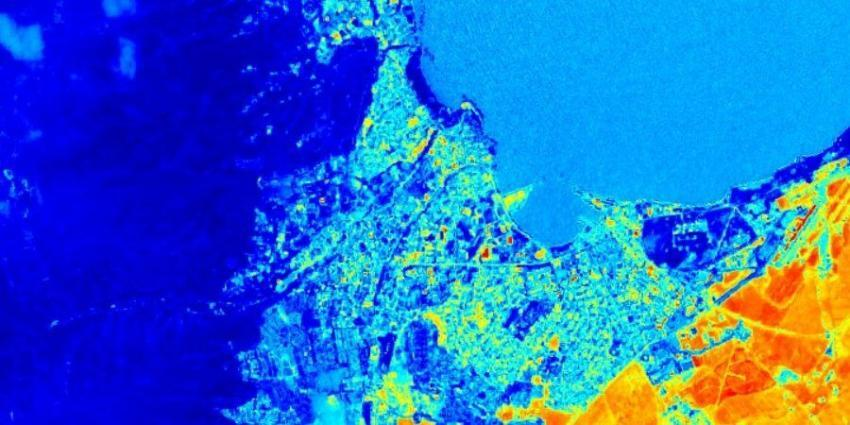
\includegraphics[width=0.6\textwidth]{Immagini/Satelliti/Sentinel-2-Moisture-Index-850x425.jpg}
        \caption{Rappresentazione Moisture Index.}
    \end{figure}

\end{itemize}


    
    
    %%==========[CAPITOLO IV]==========%%
    \chapter{Reti Neurali Artificiali (ANN)}
In questo capitolo viene posta l’attenzione sulle caratteristiche dell’apprendimento 
profondo tramite reti neurali. In particolare, si partirà dallo studio
 di una rete neurale biologica, dalla quale hanno preso ispirazione le tecniche
 fondamentali di Deep Learning, fino ad arrivare ad architetture più complicate.
    \section{La Rete Neurale Biologica}
Il miglior modo per capire il funzionamento di una rete neurale è capire come 
funziona un neurone biologico. In quanto le reti neurali artificiali traggono 
ispirazione dal funzionamento dei neuroni che compongono il cervello umano 
\cite{PARAGONE_CERVELLE_RETE_NEURALE_1, PARAGONE_CERVELLE_RETE_NEURALE_2}.

\begin{figure}[h]
    \centering
    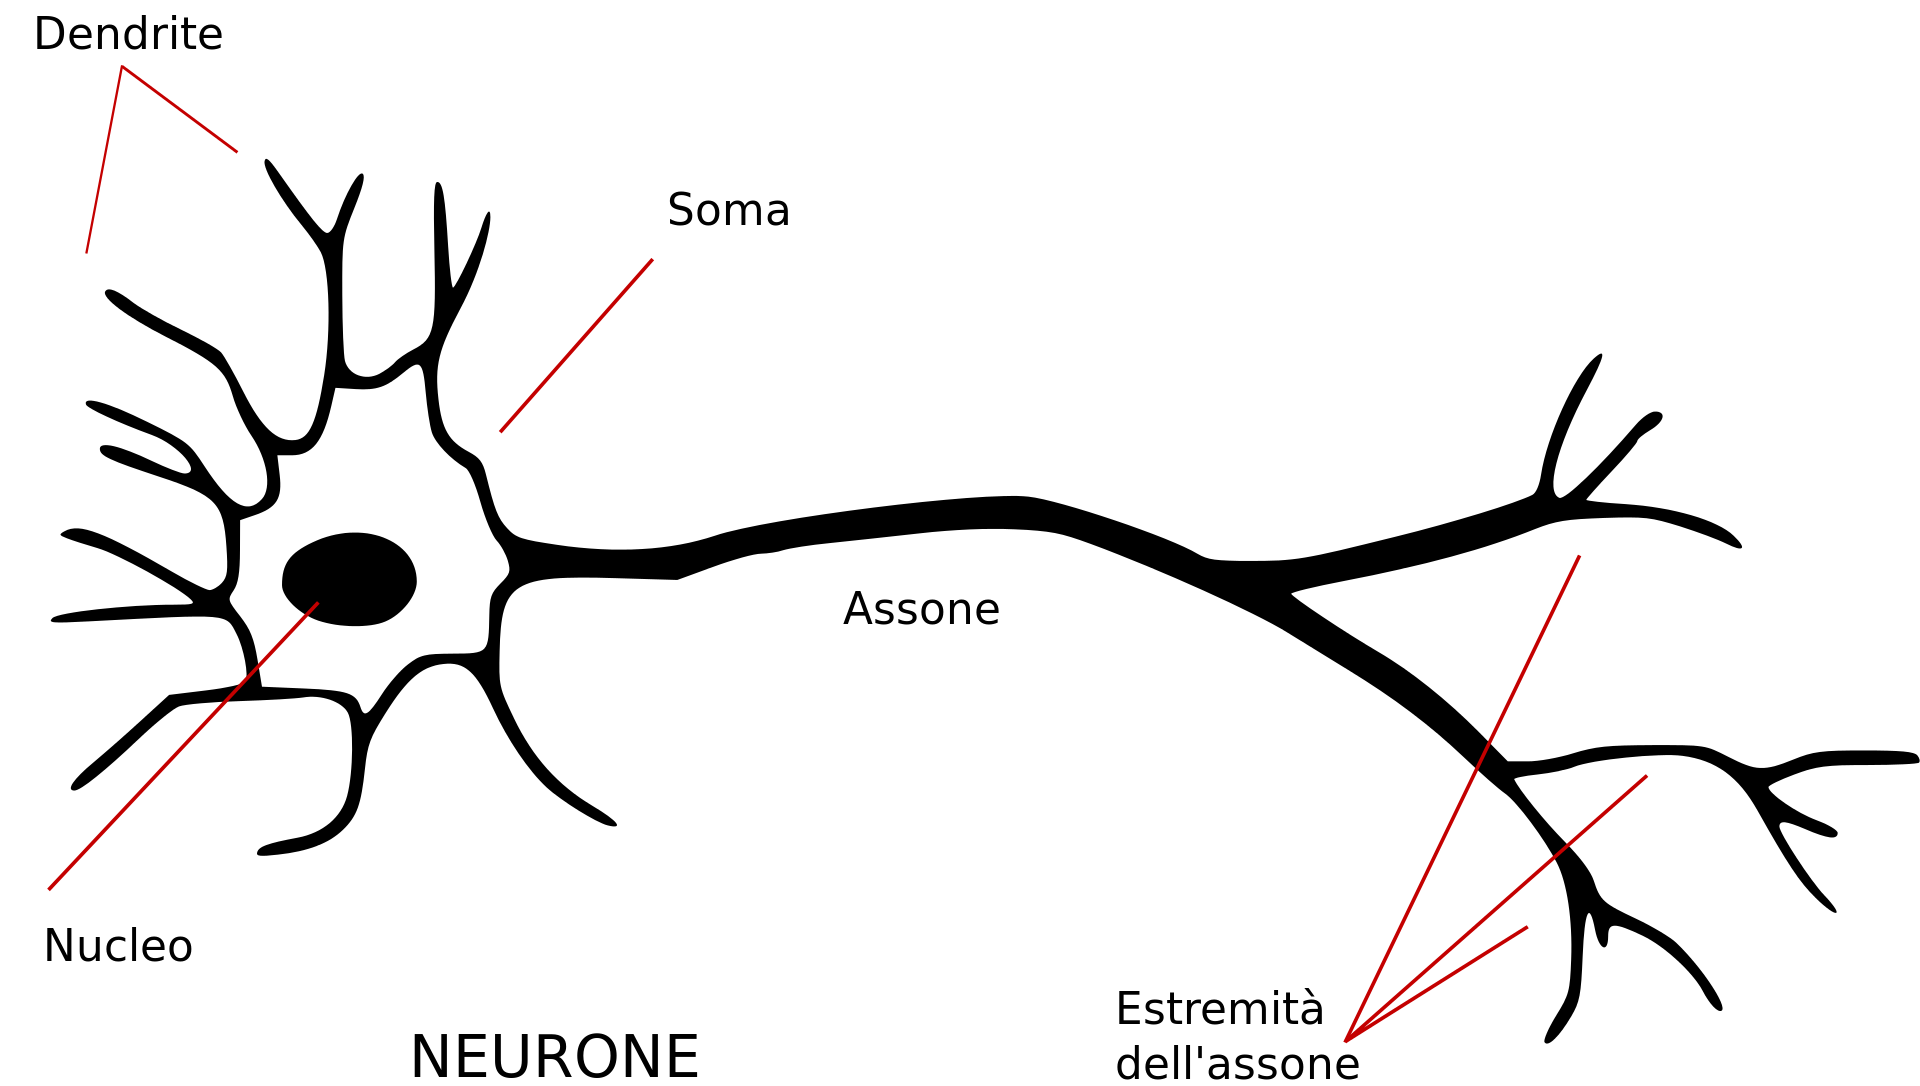
\includegraphics[width=0.75\textwidth]{Immagini/Generiche/Neurone.png}
    \caption{Esempio schematico di un neurone \cite{NEURONE_BIOLOGICO}.}
    \label{fig:esempioNeurone}
    %Figura 2.1: Esempio schematico di un neurone
\end{figure}

Infatti, un neurone, è un’unità che si occupa di compiere operazioni sulla base di
stimoli esterni e di propagare a sua volta lo stimolo.
Come si osserva dalla figura 2.1, un neurone, è composto da 3 parti principali:

\begin{itemize}
    \item  Il \textbf{soma}:  è il corpo cellulare. Si occupa di integrare tra loro i vari input
    corrispondenti agli stimoli esterni.

    \item L'\textbf{assone}:  l’unica linea di uscita del neurone che si dirama in migliaia di
    parti. Il soma restituisce un risultato che, nel caso in cui superi una certa
    soglia, il neurone si attiva e il cosiddetto "potenziale d’azione" (impulso
    elettrico) viene trasportato dall’assone. Al contrario, se il risultato non
    supera il valore di soglia il neurone rimane in uno stato di riposo.

    \item Il \textbf{dendrite}:  linea di entrata del neurone che riceve segnali in ingresso
    da altri assoni tramite le sinapsi, le quali a loro volta consentono la
    comunicazione con altri neuroni.
\end{itemize}

Il neurone è capace di ricevere segnali attraverso i propri dendriti, li elabora 
nel soma e successivamente trasmette il segnale, tramite l’assone, al neurone 
successivo. L’assone non è direttamente collegato ai dendriti di altri neuroni: 
il punto in cui il segnale viene trasmesso da una cellula ad un’altra è un 
piccolo spazio denominato “fessura sinaptica”. Quando un segnale è nei 
pressi di una sinapsi, questa rilascia un quantitativo di sostanze chimiche
chiamate “neurotrasmettitori”, i quali determinano la conduttività di una 
sinapsi, ovvero quanto la sinapsi attenua o enfatizza il segnale elettrico 
dall’assone. Nella trasmissione di un segnale, le correnti si possono sommare 
in spazio e tempo e se tale somma oltrepassa una certa soglia, un impulso di 
una certa entità e durata, denominato “potenziale d’azione”, è generato. Il 
segnale così prosegue per il prossimo assone, ricominciando il 
processo \cite{NEURONE_BIOLOGICO}.
% Le reti neurali si basano sulla simulazione di neuroni artificiali opportunamente 
% collegati, i quali ricevono in ingresso degli stimoli elaborandoli di conseguenza.
    

\section{Il Modello McCulloch-Pitts}
Nel 1943, Warren McCulloch, neurofisiologo statunitense e Walter Pitts, matematico statunitense, 
proposero un modello matematico che descriveva il funzionamento di un neurone.
ll loro modello si basava su una regola di \textbf{attivazione binaria}: se la combinazione 
dei segnali in ingresso al neurone supera una certa soglia, il neurone si attiva e 
produce un’uscita. Se non la supera, il neurone rimane a 
riposo (il famoso \textbf{“tutto-o-nulla”}) \cite{STORIA_PERCETTONE, 
IMAMGINE_MODELLO_MAT_NEURONE_GENERALE_PERCETTONE, MODELLO_E_FUNZIONAMNETO_REURONE_BIOLOGICO}.

% \begin{figure}[H]
%     \centering
%     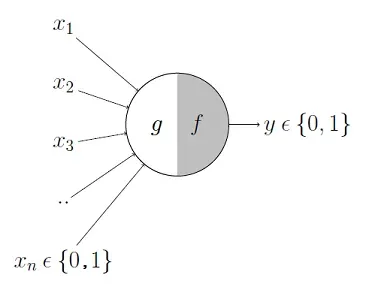
\includegraphics[width=0.5\textwidth]{Immagini/Generiche/ModelloNeurone.png}
%     \caption{Rappresentazione del modello}
%     \label{fig:modelloNeurone}
%     %Figura 2.1: Esempio schematico di un neurone
% \end{figure}
\begin{figure}[H]
    \centering
    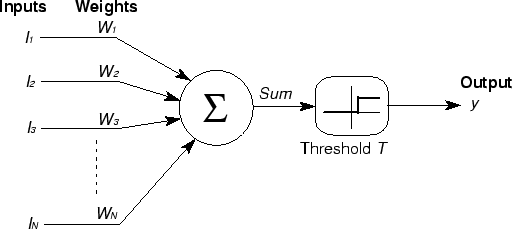
\includegraphics[width=0.75\textwidth]{Immagini/Generiche/PercettroneBinario.png}
    \caption{Rappresentazione del modello \cite{IMAMGINE_MODELLO_MAT_NEURONE_GENERALE_PERCETTONE}}
    \label{fig:modelloNeurone}
    %Figura 2.1: Esempio schematico di un neurone
\end{figure}

L’elaborazione prevedeva nel moltiplicare ogni input per un valore specifico, detto “peso”. 
I risultati di queste moltiplicazione venivano poi sommati. 
Se tale somma supera una certa soglia, allora il neurone attivava la 
propria uscita. Formalmente, questa operazione può essere descritto come
\cite{MODELLO_E_FUNZIONAMNETO_REURONE_BIOLOGICO}:

\begin{equation}
    g(x_1, x_2,\dots,x_n) = g(X) = \sum_{i=1}^{n}x_i \cdot w_i
\end{equation}
\begin{equation}
    y = f(g(X)) =
    \begin{cases} 
    1 & \text{se } g(X) \ge \theta, \\ 
    0 & \text{se } g(X) < \theta.
    \end{cases}
\end{equation}

\newpage
Dove:
\begin{itemize}
    \item $ \theta $ = soglia di attivazione
    \item $ y $ = output attivo/spento (1/0)
    \item $ x_i $ = i-esimo ingresso attivo/spento (1/0)
    \item $ w_i $ = i-esimo peso
\end{itemize}




% \begin{equation}
%     y =
%     \begin{cases} 
%     1 & \text{se } \sum_{i=1}^n w_i x_i \geq \theta, \\ 
%     0 & \text{altrimenti}.
%     \end{cases}
% \end{equation}


La distribuzione dei valori dei pesi varia in  base all’importanza 
dell’ingresso: un ingresso importante avrà un peso elevato, a 
differenza di uno meno importante che avrà un valore inferiore. 
Tuttavia, tale modello non si rivelò molto pratico, in quanto, per avere i valori 
desiderati, bisognava impostare manualmente pesi e connessioni.
Alcune semplici operazioni logiche che possono essere eseguite con questo modello sono 
\cite{STORIA_PERCETTONE}:

\begin{itemize}
    \item \textbf{AND$(x_1, x_2,\dots x_n)$}: il neurone si attiva 
    solo se tutti gli input sono attivi. Ovvero, se consideriamo 2 
    input, è necessario che $y \ge 2 $, poiché ogni input attivo da un 
    contributo di 1 e la somma è 2.

    \item \textbf{OR$(x_1, x_2,\dots x_n)$}: il neurone si attiva se 
    almeno uno degli input è attivo. Ovvero, considerando 2 input, è 
    necessario che $y \ge 1 $, poiché basta un neurone attivo che dia un 
    contributo di 1.
 
\end{itemize}

\section{Il Percettrone}
Solo successivamente nel 1958, Frank Rosenblatt, uno psicologo statunitense, propose il
modello \textbf{perceptron} (percettrone), in un report intitolato “The Perceptron: A Perceiving and Recognizing Automaton”.
Questo modello è considerato come una delle prime architetture di reti neurali artificiali 
che riprende la logica utilizzata nel modello di McCulloch e Pitts, ma leggermente più complesso.
L’innovazione principale rispetto al modello di McCulloch-Pitts riguardava l'utilizzo di valori numerici reali, 
come input, superando la limitazione all'impiego esclusivo di dati binari. 
Inoltre, i valori dei pesi associati a ciascun input venivano appresi mediante una 
regola di apprendimento che 
tiene conto della differenza tra output del neurone e output desiderato
\cite{ASPETTI_APPRENDIMENTO_PERCETTONE,STORIA_PERCETTONE,ARTICOLO_PERCETTONE,
IMAMGINE_MODELLO_MAT_NEURONE_GENERALE_PERCETTONE}.

\begin{figure}[H]
    \centering
    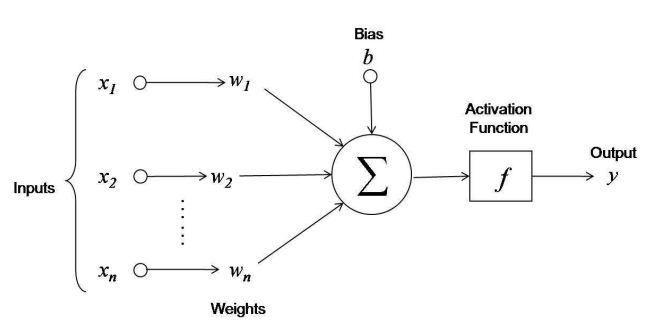
\includegraphics[width=0.75\textwidth]{Immagini/Generiche/neuron_representation_cornell.jpeg}
    \caption{Rappresentazione del modello \cite{IMMAGINE_PERCETTRONE_ASPETTI}}
    \label{fig:modelloNeurone2}
    %Figura 2.1: Esempio schematico di un neurone
\end{figure}

Un percettrone può essere visto come un classificatore lineare; cioè un algoritmo 
che classifica l'input separando due categorie tracciando una linea retta (o un iperpiano in spazi a dimensioni superiori).
Per questa ragione, il perceptron è considerato un passo cruciale nello sviluppo 
degli algoritmi di apprendimento automatico. 

Matematicamente, il funzionamento del perceptron può essere espresso attraverso 
le seguenti formule \cite{FORMULE_PERCETTRONE}:
\begin{equation}
    z = \sum_{i=1}^{n} w_i x_i + b = (x_1 \cdot w_1)\ + (x_2 \cdot w_2)\ + ...\ + (x_n \cdot w_n) + b 
\end{equation}
\begin{equation}
    y = \hat{y}= f\left(z\right)
\end{equation}

Dove:
\begin{itemize}
    \item \(x_i\) rappresenta il valore di ciascun input;
    \item \(w_i\) è il peso associato all'input \(x_i\);
    \item \(b\) è il bias, un termine aggiuntivo che permette di traslare la funzione di attivazione;
    \item \(f\) è una funzione di attivazione, generalmente una soglia (ad esempio, una funzione scalino) che 
    determina l'output finale del modello. Una delle funzioni più utilizzate è l'\textbf{Heaviside step function}:
    \[f(z) =
        \begin{cases} 
        1 & \text{if } z \ge 0, \\ 
        0 & \text{if } z < 0.
        \end{cases}
    \]
    
    \item \(y\) rappresenta l'output del modello, che spesso viene indicato anche come \(\hat{y}\) per denotare un valore stimato o predetto.
\end{itemize}

Spesso, per rappresentare le operazioni in una maniera più compatta e generalizzata, si adotta 
una rappresentazione vettoriale, in cui i valori degli input e dei pesi sono rappresentati come segue:
\[
    \mathbf{X} = \begin{bmatrix} x_1 \\ x_2 \\ \vdots \\ x_n \end{bmatrix}, \quad
    \mathbf{W} = \begin{bmatrix} w_1 \\ w_2 \\ \vdots \\ w_n \end{bmatrix}
\]
    
%i valori di input (\(x_i\)) sono rappresentati dal vettore \(\mathbf{X}\), mentre i pesi (\(w_i\)) sono rappresentati dal vettore \(\mathbf{W}\).
Utilizzando questa notazione, la formula che descrive il funzionamento del perceptron in 
forma vettoriale è definita come:

\begin{equation}
    \begin{split}
        \hat{y} &= f\left( \mathbf{X}^\top \mathbf{W} + b \right)
        = f\left( 
        \begin{bmatrix} x_1 & x_2 & \cdots & x_n \end{bmatrix} \cdot
        \begin{bmatrix} w_1 \\ w_2 \\ \vdots \\ w_n \end{bmatrix}
        + b
        \right)%= \\
        % &= f\left( (x_1 \cdot w_1) + (x_2 \cdot w_2) + \dots + (x_n \cdot w_n) + b \right) = f(z + b)
    \end{split}
    \label{eq:formulaPercettroneVettoriale}
\end{equation}

\subsection{L'Algoritmo di Apprendimento del Percettrone}
Rosenblatt dimostrò che l’algoritmo di apprendimento del percettrone converge se le
 due classi sono linearmente separabili, ovvero se esiste un iperpiano lineare che separi
 correttamente le due classi.
L'algoritmo di apprendimento del percettrone si basa su un approccio iterativo di 
ottimizzazione dei pesi. Durante l'addestramento, i pesi vengono aggiornati sulla 
base dell'errore tra l'uscita prevista e l'uscita reale. Tale processo di aggiornamento 
dei pesi può essere descritto tramite la seguente regola 
\cite{APPRENDIMENTO_PRECETTRONE,ASPETTI_APPRENDIMENTO_PERCETTONE,IMAMGINE_MODELLO_MAT_NEURONE_GENERALE_PERCETTONE}:

\begin{equation}
    w_i = w_i + \eta(y - \hat{y}) x_i
    \label{eq:apprendimentoPercettrone}
\end{equation}

dove:
\begin{itemize}
    \item \( \eta \) è una costante che determina il tasso di apprendimento. \\Questo 
    valore è noto anche come \textbf{learning rate};
    \item \( y \) è il valore atteso;
    \item \( \hat{y} \) è il valore predetto dal percettrone;
    \item \( x_i \) è l'input associato al peso \( w_i \).
\end{itemize}

\subsection{Implementazione di un percettrone}
Per comprendere il funzionamento di questo modello, proviamo a implementare un 
percettrone utilizzando un linguaggio di programmazione e 'addestrarlo' a distinguere 
i punti separati da una retta.

\hspace{0.25cm}

Per la parte di algebra lineare useremo la libreria \textbf{numpy}. Mentre per realizzare i
vari grafici useremo la libreria \textbf{matplotlib}.
\begin{lstlisting}
import numpy as np
import random
import matplotlib as plt
\end{lstlisting}

Basandosi sulle formule \eqref{eq:apprendimentoPercettrone} e \eqref{eq:formulaPercettroneVettoriale}, 
il percettrone può essere modelizzato nel seguente modo:

\begin{lstlisting}

    class Perceptron:

        def __init__(self, inputs: int) -> None:
            self.W: np.array = np.random.rand(inputs) 
            self.b: float = random.random()

        def heaviSideStep(self, z: float) -> int:
            return 1 if z >= 0.0 else 0

        def predict(self, X: np.array) -> int:
            z = np.dot(self.W, X) + self.b  # Somma pesata
            y_hat = self.heaviSideStep(z)
            return y_hat
        
        def train(self, lr: float, epochs: int, Y_train: np.array, X_train: np.array) -> Tuple[np.array, np.array]:
        
            train_losses: List[float] = []
            epoch_avg_loss: List[float] = []

            for epoch in range(epochs):
                epoch_loss: List[float] = []

                for i, X in enumerate(X_train):
                    y_hat = self.predict(X)

                    # Calcolo dell'errore
                    error = Y_train[i] - y_hat  

                    # Aggiornamento dei pesi e del bias
                    self.W += lr * error * X
                    self.b += lr * error

                    # Salva l'errore
                    epoch_loss.append(error)

                # Errore medio per epoca
                epoch_avg_loss.append(np.mean(epoch_loss))
                train_losses.extend(epoch_loss)

            return np.array(train_losses, dtype=np.float32), np.array(epoch_avg_loss, dtype=np.float32)
\end{lstlisting}

Per svolgere l'addestramento del percettrone, utilizziamo la funzione "train", alla 
quale forniamo un set di dati per il quale conosciamo già il risultato corretto. Durante 
l'addestramento, l'errore (o loss) viene calcolato per ogni esempio del set di 
dati, aggiornati di conseguenza i pesi ed il bias. 

I dati di esempio vengono utilizzati più volte. Ogni iterazione completa sul set di 
dati è chiamata \textbf{epoca} (epoch).

Durante questa procedura teniamo anche traccia di tutti i valori, in modo che poi possiamo 
utilizzarli per visualizzare l'andamento.
\newpage
Iniziamo a definire i parametri 
\begin{lstlisting}
N_TRAIN: int = 5000
N_TEST: int = 2000
INPUT_SIZE: int = 2
MIN: int = -2
MAX: int = 12

alpha: float = -2
x_offset: float = -5
y_offset: float = +5

X_TRAIN = np.random.uniform(MIN, MAX, (N_TRAIN, 2))  # N punti casuali (x, y)
X_TEST = np.random.uniform(MIN, MAX, (N_TEST, 2))
Y_TRAIN = np.array([1 if x2 > alpha*(x1 + x_offset) + y_offset else 0 for x1, x2 in X_TRAIN])


perceptron = Perceptron(inputs=INPUT_SIZE)
print("Pesi iniziali:", perceptron.W)
print("Bias iniziale:", perceptron.b)

\end{lstlisting}


% \begin{figure}[H]
%     \centering
%     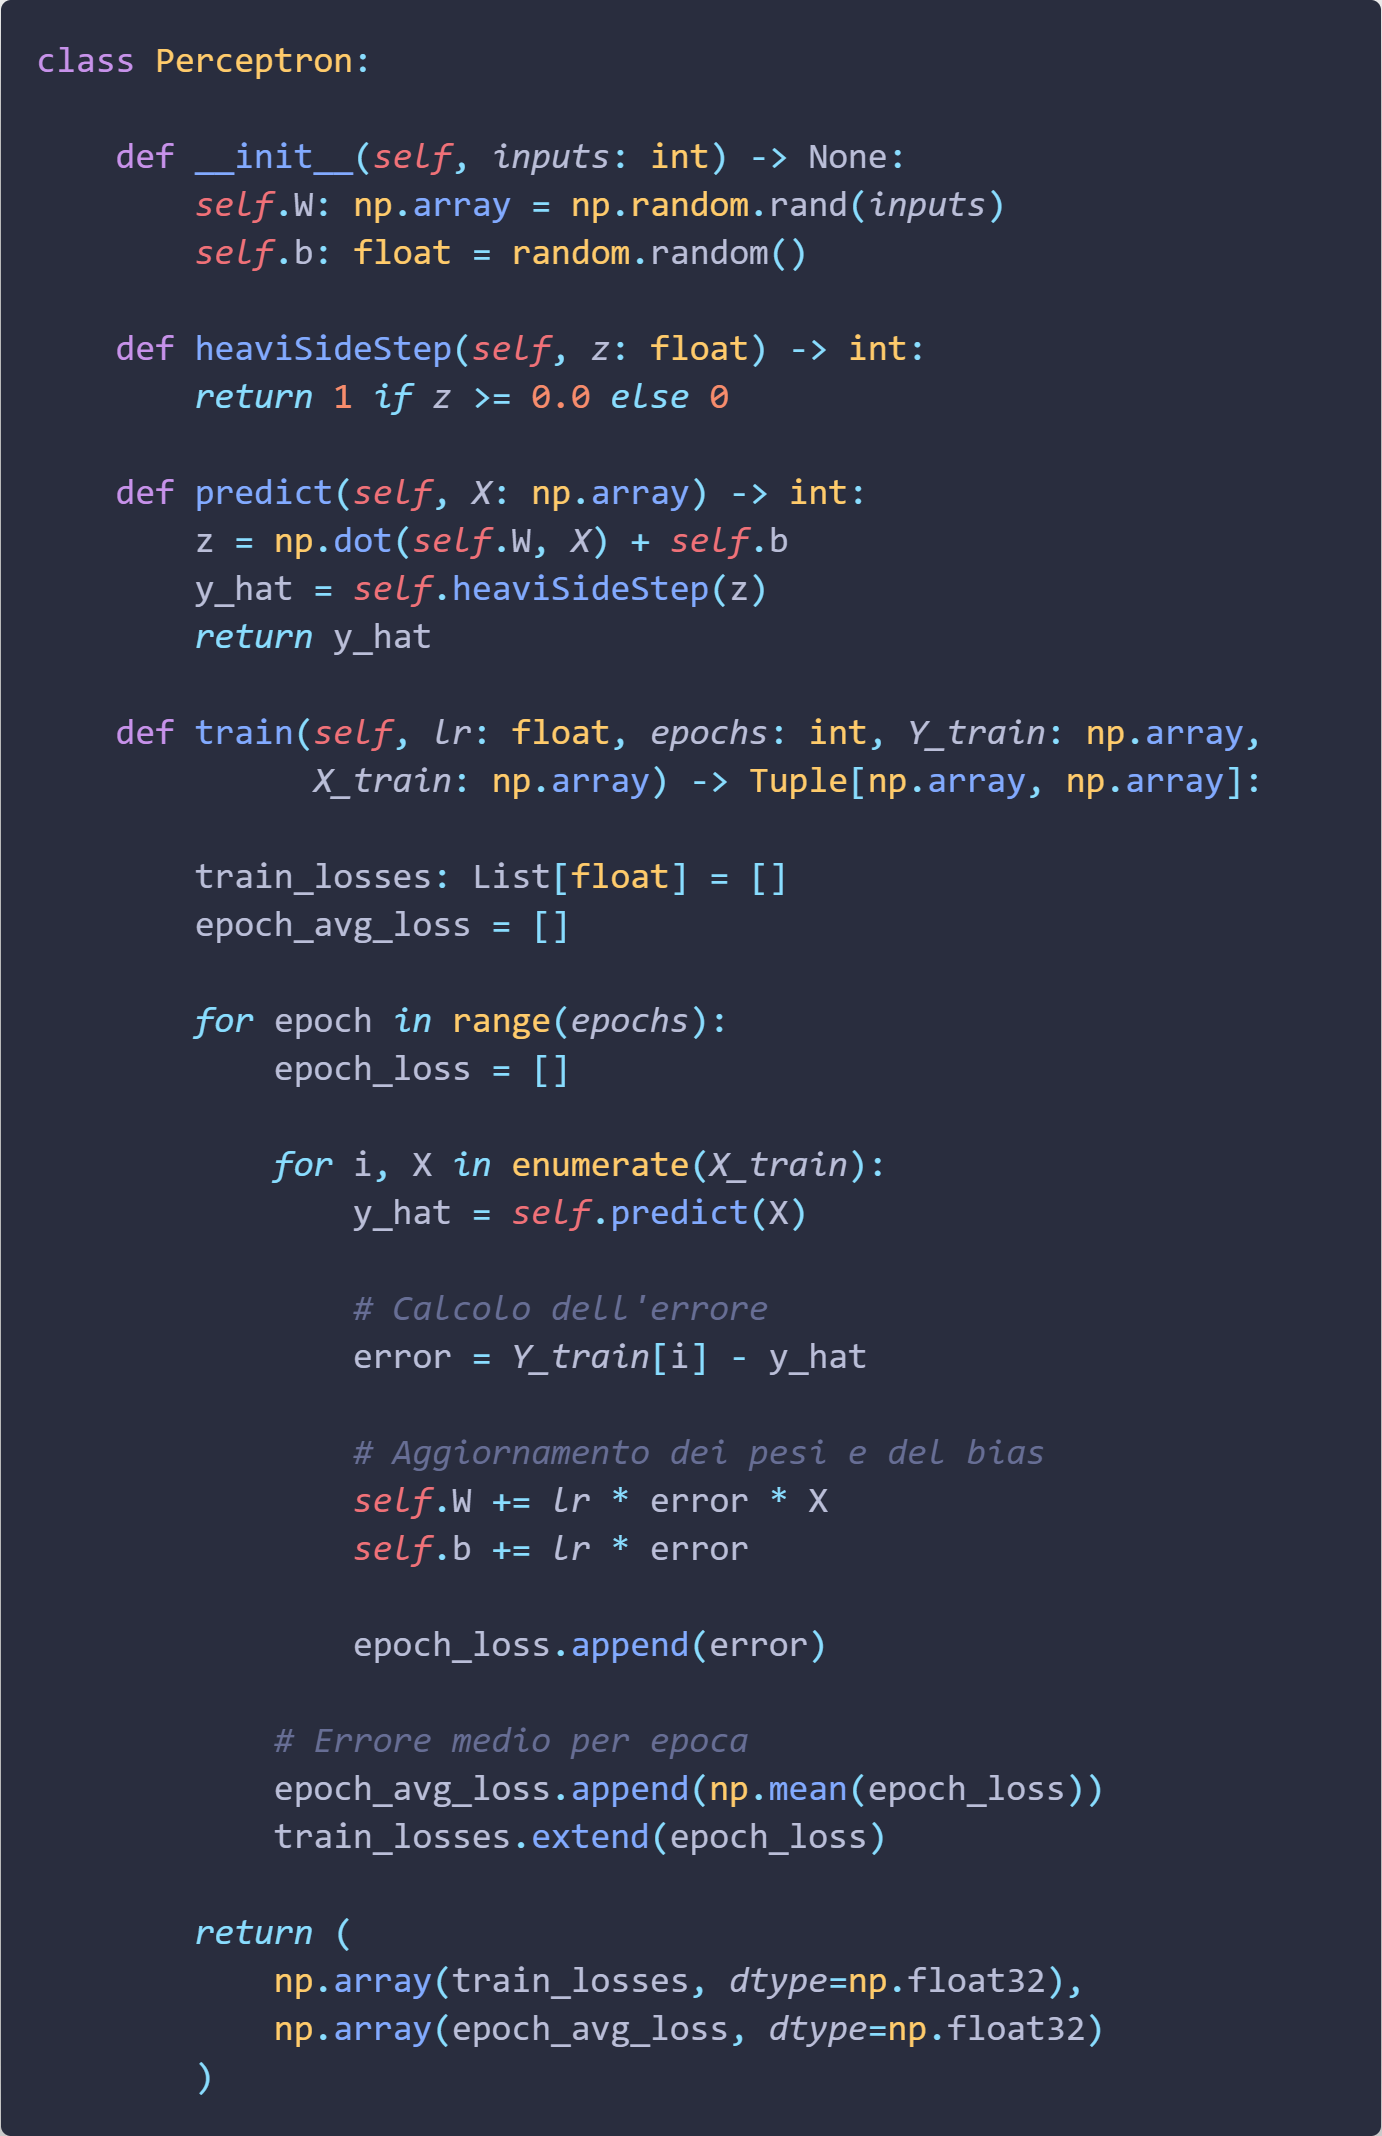
\includegraphics[width=0.8\textwidth]{Immagini/Codice/Perceptron.png}
%     %\caption{Grafico del problema dello XOR}
%     %\label{fig:Modellazione }
%     %Figura 2.1: Esempio schematico di un neurone
% \end{figure}

Pesi iniziali: [0.80801983, 0.46388153]
\newline
Bias iniziale: 0.7213280952626825

\hspace{0.25cm}

Ora chiamiamo la procedura per svolgere il training passandogli i vari parametri.
\begin{lstlisting}
# Training
train_losses, epoch_avg_loss = perceptron.train(lr=1e-3, epochs=30, Y_train=Y_TRAIN, X_train=X_TRAIN)

print("Pesi finali:", perceptron.W)
print("Bias finale:", perceptron.b)
\end{lstlisting}

Pesi finali: [0.06009108, 0.03008616]\\
Bias finale: -0.4496719047373185

\hspace{0.25cm}

Mentre per quanto riguarda il valore del piano tracciato dal percettrone, possiamo calcolarlo nel
seguente modo:
\begin{lstlisting}
slope = -perceptron.W[0] / perceptron.W[1]
intercept = -perceptron.b / perceptron.W[1]
\end{lstlisting}


\newpage

Così è come appare la classificazione dei casi di test prima della procedura di addestramento.

\begin{figure}[H]
    \centering
    \includegraphics[width=0.80\textwidth]{Immagini/Grafici/EsempioApplicativoPercettrone_parte1.png}
    \caption{Grafico prima dell'addestramento}
    \label{fig:Modellazione1 }
    %Figura 2.1: Esempio schematico di un neurone
\end{figure}

La linea tratteggiata è la retta che voglio approssimare con il percettrone, mentre 
quella viola è la retta attuale del percettrone.
Finita la procedura di addestramento, il grafico appare così
\begin{figure}[H]
    \centering
    \includegraphics[width=0.80\textwidth]{Immagini/Grafici/EsempioApplicativoPercettrone_parte2.png}
    \caption{Grafico dopo l'addestramento}
    \label{fig:Modellazione2 }
    %Figura 2.1: Esempio schematico di un neurone
\end{figure}

Come si può osservare dei grafici \ref{fig:Modellazione1 } e \ref{fig:Modellazione2 }, 
il percettrone è riuscito ad "imparare" 
a classificare correttamente i punti di test, raggiungendo un precisione molto vicina al 100\%.

Il grafico sottostante mostra l'andamento dell'errore medio di ogni epoca 
durante la fase di addestramento.

\begin{figure}[H]
    \centering
    \includegraphics[width=1\textwidth]{Immagini/Grafici/EsempioApplicativoPercettroneLOSS.png}
    \caption{Grafico della loss}
    \label{fig:Modellazione3 }
    %Figura 2.1: Esempio schematico di un neurone
\end{figure}

% \begin{minted}[linenos, frame=lines, bgcolor=lightgray]{python}
% # Esempio di codice Python
% def somma(a, b):
%     """
%     Questa funzione restituisce la somma di due numeri.
%     """
%     return a + b

% print(somma(3, 5))
% \end{minted}





\subsection{Limiti del percettrone}
Nel 1969, Marvin Minsky e Symour A. Papert, nel loro libro “Perceptrons: an 
introducion to computational geometry”, dimostrarono matematicamente tutte le 
principali limitazioni 
del percettrone. 
Una di queste limitazioni riguardava l'incapacità del percettrone di gestire 
problemi non linearmente separabili \cite{ARTICOLO_LIMITI_PRECETTRONE}.
% , come dimostrato dal famoso esempio dell'operatore XOR, in quanto 
% quest'ultimo non è linearmente separabile.

La figura \ref{fig:XOR_GRAPH} mostra degli esempi di classificazione svolti dall'algoritmo del
percettrone per i problemi logici AND, OR e XOR. Graficamente, la retta di decisione
determinata dal percettrone riesce a classificare in maniera corretta ciascun elemento
in input nel caso dei problemi AND e OR. A differenza degli ultimi, è possibile notare
come una retta non sia sufficiente per separare le due classi nel problema XOR: ciò
è dovuto al fatto che tale rete riesce a classificare correttamente due classi 
linearmente separabili, ma non riesce a risolvere un problema di classificazione tra classi non
linearmente separabili, quale ad esempio il problema XOR.
L'unico modo consisterebbe nel dividere il piano in 3 aree utilizzando due rette di decisione, 
ma questo non è minimamente possibile utilizzando esclusivamente un solo percettrone 
\cite{LIMITI_PERCETTRONE, MODELLO_E_FUNZIONAMNETO_REURONE_BIOLOGICO}.

\begin{figure}[H]
    \centering
    \includegraphics[width=1\textwidth]{Immagini/Grafici/graficiLimitiPercettrone.png}
    \caption{Esempi di classificazione \cite{LIMITI_PERCETTRONE}.}
    \label{fig:XOR_GRAPH}
    %Figura 2.1: Esempio schematico di un neurone
\end{figure}



% \begin{figure}[H]
%     \centering
%     \includegraphics[width=0.60\textwidth]{Immagini/Grafici/Perceptron_XOR_v3.png}
%     \caption{Grafico del problema dello XOR}
%     \label{fig:XOR_GRAPH2}
%     %Figura 2.1: Esempio schematico di un neurone
% \end{figure}

Questa constatazione segnò l'inizio di un periodo noto come “Inverno delle IA”, durante 
il quale l'interesse per lo sviluppo delle reti neurali diminuì notevolmente.
Al fine di risolvere problemi più complessi, si cominciò ad interconnettere gli 
input dei neuroni artificiali con gli output di altri neuroni artificiali, creando 
una rete neurale a più livelli. Questo portò alla nascita 
del \textbf{Multi-layer Perceptron (MLP)} .


\section{Single-layer Perceptron (SLP)}
Il Single-layer Perceptro (percettrone a singolo layer)è un'estensione del 
percettrone singolo, in cui più percettroni sono in "pilati" per formare un unico strato (o layer). Questo permette all'SPL di poter
essere utilizzato per problemi di classificazione multiclasse.

I SLP furono utilizzati per diverse applicazioni durante gli anni '60, tuttavia, 
la scoperta dei limiti del perceptron (il libro di Minsky e Papert del 1969) 
fece calare rapidamente l'interesse per questi modelli, poiché non erano in 
grado di risolvere problemi non linearmente separabili \cite{ALL_SLP}.

\begin{figure}[H]
    \centering
    \includegraphics[width=0.60\textwidth]{Immagini/Generiche/SLP.png}
    \caption{Rappresentazione di un SLP}
    \label{fig:SingleLayerPerceptrons}
    %Figura 2.1: Esempio schematico di un neurone
\end{figure}
Come si può osservare, ogni nodo (percettrone) nello strato applica la stessa logica, 
ma in modo indipendente per calcolare diversi output.
\\Matematicamente, il funzionamento del Single-layer Perceptron è molto simile al funzionamento
del percettrone, infatti si ha che:
\begin{equation}
    z_i =  b_i + \sum_{j=1}^{m} w_{ij}\cdot x_j%= (x_1 \cdot w_1)\ + (x_2 \cdot w_2)\ + ...\ + (x_n \cdot w_n) + b 
\end{equation}
\begin{equation}
    \hat{y}_i= g\left(z_i\right)
\end{equation}

L'SLP può essere visto come una versione semplificata del MLP, pertanto non
ci soffermeremo ulteriormente.



    \section{Multi-layer Perceptron (MLP)}
\label{sec:Multilayer_Perceptro_marker}
\subsubsection{Cenni storici}
I primi tentativi teorici di estendere il perceptron a più livelli 
risalgono agli studi di Ivakhnenko e Lapa negli anni '60 e '70, ma erano 
limitati e computazionalmente costosi. Inoltre, la mancanza di un algoritmo 
efficace per aggiornare i pesi impedì progressi significativi.
Solo verso il 1986 con l'introduzione dell'algoritmo di 
retropropagazione (backpropagation), formalizzato da David Rumelhart, 
Geoffrey Hinton e Ronald Williams nel loro articolo, si aprirono nuove 
possibilità per realizzare queste tipologie di reti \cite{Articolo_backpropagation}.


\subsubsection{Struttura del modello}
l percettrone multistrato è una vera e propria rete neurale artificiale 
composta, come si evince dal nome, da più strati di percettroni. Esso si compone di 
un livello di input, il quale riceve il segnale, ed un livello di output, che esegue 
una previsione o prende una decisione per quanto concerne l’input e, tra 
questi due livelli, vi è un numero arbitrario di strati “nascosti” (hidden), il vero motore 
computazionale della rete. Ciascun neurone di un livello è connesso a tutti i 
neuroni del livello precedente, per tale motivo una rete di questo tipo è anche 
detta Fully Connected 
\cite{ASPETTI_APPRENDIMENTO_PERCETTONE,GradientDescent_NeuralNetworks,ALL_DEEP_LEARNING}. 

\begin{figure}[H]
    \centering
    \includegraphics[width=0.8\textwidth]{Immagini/Generiche/MLP_v2.jpg}
    \caption{Esempio di un MLP \cite{Immagine_MLP}.}
    \label{fig:MLP_GRAPH3}
    %Figura 2.1: Esempio schematico di un neurone
\end{figure}

Nel corso dell’ultimo decennio è diventato sempre più frequente l’utilizzo di reti 
neurali aventi molteplici \textit{hidden layer}. Una rete neurale avente più di 
un \textit{hidden layer} è detta anche \textbf{rete neurale profonda (deep neural network)} e l’insieme di queste 
reti costituiscono la base del moderno \textit{deep learning}.
Spesso ci si riferisce a questi modelli anche con \textit{feed forward network}.

\subsection{Rappresentazione matematica del modello}
Un Multi-Layer Perceptron (MLP) può essere formalizzato matematicamente 
come una sequenza di trasformazioni lineari, seguite da funzioni di attivazione 
non lineari. 
\subsubsection{Notazione}
Prima di passare a definire le formule modello, vediamo la notazione
utilizzata dal modello 
\cite{GradientDescent_NeuralNetworks,ALL_DEEP_LEARNING,ASPETTI_MLP_1,ASPETTI_MLP_2}:

\begin{itemize}
    \item Il numero di livelli (o layer) della rete sono denotati con $L$,
    e per riferirsi ad un layer generico, useremo la lettera $l$, con $l\in [0, L]$; 

    \item Con la notazione $n_l$ ci si riferisce al numero di percettroni (o neuroni)
    che compongono un generico livello $l$;

    \item Con $h^{(l)}$ si indica il vettore colonna dei risultati delle funzioni 
    di attivazione calcolate al livello $l$;

    \item Per rappresentare gli input della rete viene utilizzato un vettore colonna di dimensione $d$,
    dove $d$ rappresenta il numero degli input della rete:
    
    \[
        \mathbf{X} = \begin{bmatrix} x_1 \\ x_2 \\ \vdots \\ x_n \end{bmatrix} \in \mathbb{R}^d
    \]

    \item Per rappresentare i pesi di ogni layer $l$, viene utilizzata una matrice $\mathbf{W}^{(l)}$ di dimensioni
    $n_l \times n_{l-1}$, dove $n_l$ è il numero di neuroni nel livello corrente 
    e $n_{l-1}$ è il numero di neuroni nel livello precedente:
    
    \[
        \mathbf{W}^{(l)} = 
        \begin{bmatrix}
        w_{11}^{(l)} & w_{12}^{(l)} & \cdots & w_{1n_{l-1}}^{(l)} \\
        w_{21}^{(l)} & w_{22}^{(l)} & \cdots & w_{2n_{l-1}}^{(l)} \\
        \vdots & \vdots & \ddots & \vdots \\
        w_{n_l1}^{(l)} & w_{n_l2}^{(l)} & \cdots & w_{n_ln_{l-1}}^{(l)}
        \end{bmatrix}
        \in \mathbb{R}^{n_l \times n_{l-1}}
    \]

    In questa matrice, ogni colonna rappresenta i pesi degli input associati a
    un singolo percettrone (o neurone) del layer;
    

    \item Per ogni livello $l$, il bias è rappresentato come un vettore 
    colonna di dimensioni $n_l$:
    
    \[
        \mathbf{b}^{(l)} = 
        \begin{bmatrix}
        b_1^{(l)} \\
        b_2^{(l)} \\
        \vdots \\
        b_{n_l}^{(l)}
        \end{bmatrix}
        \in \mathbb{R}^{n_l}
    \]

    \item Per denotare la funzione di attivazione usata al livello $l$, si
    utilizza la notazione $\boldsymbol{\sigma^{(l)}}$. Pertanto, ogni percettrone (o neurone) 
    del livello $l$ utilizzerà la stessa funzione di attivazione.
    
\end{itemize}
\subsubsection{Funzionamento}
Chiarita la notazione utilizzata, ora possiamo passare a vedere le formule che
caratterizzato il funzionamento del modello 
\cite{GradientDescent_NeuralNetworks,ALL_DEEP_LEARNING,ASPETTI_MLP_1,ASPETTI_MLP_2}:
\begin{itemize}
    % \item L'output di ogni livello $l$ viene calcolato come una combinazione 
    % lineare degli input, seguita dall'applicazione della 
    % funzione di attivazione:

    \item L'output di ogni livello \( l \) viene calcolato come una combinazione 
    lineare degli input, che dipende dai pesi del layer, dal bias e dal risultato del 
    livello precedente, seguita dall'applicazione della funzione di attivazione:
    
    \begin{equation}
        \mathbf{h}^{(l)} = \boldsymbol{\sigma^{(l)}}\left( \mathbf{W}^{(l)} \mathbf{h}^{(l-1)} + \mathbf{b}^{(l)} \right)
        \label{MPL_LAYER}
    \end{equation}
    
    Per il livello iniziale ($l=0$), il vettore di input $\mathbf{h}^{(0)}$ è sostituito da $\mathbf{X}$, il vettore degli input della rete.
   
    \item L'output finale (o predetto) della rete $\hat{\mathbf{y}}$ è calcolato al livello $L$ come:
    \begin{equation}
        \hat{\mathbf{y}} = \boldsymbol{\sigma}^{(L)}\left( \mathbf{W}^{(L)} \mathbf{h}^{(L-1)} + \mathbf{b}^{(L)} \right)
        \label{MPL_OUTPUT}
    \end{equation}
   

\end{itemize}

\newpage
\subsection{Esempio applicativo}
Consideriamo un MPL con la seguente struttura:
\begin{figure}[H]
    \centering
    \includegraphics[width=0.65\textwidth]{Immagini/Generiche/esempioAplicativo_MPL.png}
    \caption{Esempio di un MLP.}
    
    %Figura 2.1: Esempio schematico di un neurone
\end{figure}

Come si osserva dalla figura, la rete è costituita dai seguenti elementi:

\begin{itemize}
    \item 3 neuroni in input (\(x_1, x_2, x_3\));
    \item Un livello nascosto (\(l=1\)) con 3 neuroni (\(h_1^{(1)}, h_2^{(1)}, h_3^{(1)}\));
    \item Un livello di output (\(l=2\)) con 2 neuroni (\({y}_1, {y}_2\)).
\end{itemize}

Definiamo i parametri della rete come segue:
\begin{itemize}
    \item Vettore di input: 
    \[\mathbf{X} = \begin{bmatrix} x_1 \\ x_2 \\ x_3 \end{bmatrix} =\begin{bmatrix} 1 \\ -2 \\ 0.5 \end{bmatrix}\]


    \item Matrici dei pesi: 
    \begin{multicols}{2}
        {
            \[
                \mathbf{W}^{(1)} = 
                \begin{bmatrix}
                    0.2 & -0.4 & 0.1 \\
                    -0.1 & 0.3 & -0.5 \\
                    0.7 & 0.2 & -0.3
                \end{bmatrix}
            \]
        }
        {
            \[
                \mathbf{W}^{(2)} = 
                \begin{bmatrix}
                    0.5 & -0.6 & 0.2 \\
                    -0.3 & 0.8 & -0.7
                \end{bmatrix}
            \]
        }
    \end{multicols}
    
    \item Vettori dei bias: 
    \begin{multicols}{2}
        {\[\mathbf{b}^{(1)} = \begin{bmatrix} 0.1 \\ -0.2 \\ 0.3 \end{bmatrix}\]}
        {\[\mathbf{b}^{(2)} = \begin{bmatrix} -0.1 \\ 0.4 \end{bmatrix}\]}
    \end{multicols}

    
    \item Come funzione di attivazione per $\sigma^{(1)}$ e per $\sigma^{(2)}$, utilizzeremo la funzione di \textbf{Heaviside} 
    con $\theta = 0$, definita nel seguente modo:
    \[
        \sigma(z) = 
        \begin{cases} 
        1 & \text{se } z \geq \theta, \\
        0 & \text{se } z < \theta.
        \end{cases}
    \]
\end{itemize}

\newpage
Ora passiamo a calcolare l'output della rete.
Utilizzando le formule \ref{MPL_LAYER} e \ref{MPL_OUTPUT}, l'output della rete 
può essere descritto come:

\[
    {\mathbf{y}} = \sigma^{(2)}\left( \mathbf{W}^{(2)}\left(\sigma^{(1)}\left( \mathbf{W}^{(1)}\mathbf{X} + {\mathbf{b}}^{(1)}\right)  \right)+ {\mathbf{b}}^{(2)}\right)
\]
\\
Iniziamo calcolando il prodotto matriciale \(\mathbf{W}^{(1)}\mathbf{X}\):

\[
\mathbf{W}^{(1)} \mathbf{X} = 
\begin{bmatrix}
0.2 & -0.4 & 0.1 \\
-0.1 & 0.3 & -0.5 \\
0.7 & 0.2 & -0.3
\end{bmatrix}
\begin{bmatrix}
1 \\ -2 \\ 0.5
\end{bmatrix}
=
\begin{bmatrix}
0.2(1) + (-0.4)(-2) + 0.1(0.5) \\
-0.1(1) + 0.3(-2) + (-0.5)(0.5) \\
0.7(1) + 0.2(-2) + (-0.3)(0.5)
\end{bmatrix}
=
\]
\[
= 
\begin{bmatrix}
0.2 + 0.8 + 0.05 \\
-0.1 - 0.6 - 0.25 \\
0.7 - 0.4 - 0.15
\end{bmatrix}
=
\begin{bmatrix}
1.05 \\ -0.95 \\ 0.15
\end{bmatrix}
\]
Ora sommiamo il bias:

\[
\mathbf{W}^{(1)} \mathbf{X} + \mathbf{b}^{(1)} = 
\begin{bmatrix}
1.05 \\ -0.95 \\ 0.15
\end{bmatrix}
+
\begin{bmatrix}
0.1 \\ -0.2 \\ 0.3
\end{bmatrix}
=
\begin{bmatrix}
1.15 \\ -1.15 \\ 0.45
\end{bmatrix}
\]

Infine, applichiamo la funzione di Heaviside (con \(\theta = 0\)) in modo
da ottenere il risultato del layer 1 ($\mathbf{h}^{(1)}$):

\[
\mathbf{h}^{(1)} =
\sigma^{(1)}\left( \mathbf{W}^{(1)} \mathbf{X} + \mathbf{b}^{(1)} \right) =
\begin{bmatrix}
\sigma(1.15) \\
\sigma(-1.15) \\
\sigma(0.45)
\end{bmatrix}
=
\begin{bmatrix}
1 \\
0 \\
1
\end{bmatrix}
\]


Ora calcoliamo il prodotto \(\mathbf{W}^{(2)} \mathbf{h}^{(1)}\):

\[
\mathbf{W}^{(2)} \mathbf{h}^{(1)} = 
\begin{bmatrix}
0.5 & -0.6 & 0.2 \\
-0.3 & 0.8 & -0.7
\end{bmatrix}
\begin{bmatrix}
1 \\ 0 \\ 1
\end{bmatrix}
=
\begin{bmatrix}
0.5(1) + (-0.6)(0) + 0.2(1) \\
-0.3(1) + 0.8(0) + (-0.7)(1)
\end{bmatrix}
=
\]
\[
= 
\begin{bmatrix}
0.5 + 0 + 0.2 \\
-0.3 + 0 - 0.7
\end{bmatrix}
=
\begin{bmatrix}
0.7 \\ -1.0
\end{bmatrix}
\]

Ora sommiamo il bias:

\[
\mathbf{W}^{(2)} \mathbf{h}^{(1)} + \mathbf{b}^{(2)} = 
\begin{bmatrix}
0.7 \\ -1.0
\end{bmatrix}
+
\begin{bmatrix}
-0.1 \\ 0.4
\end{bmatrix}
=
\begin{bmatrix}
0.6 \\ -0.6
\end{bmatrix}
\]

Infine, applichiamo la funzione di Heaviside al livello di output
in modo da ottenere il risultato del layer 2 (($\mathbf{h}^{(2)}$)):

\[
\mathbf{h}^{(2)}=
\sigma^{(2)}\left( \mathbf{W}^{(2)} \mathbf{h}^{(1)} + \mathbf{b}^{(2)} \right) =
\begin{bmatrix}
\sigma(0.6) \\
\sigma(-0.6)
\end{bmatrix}
=
\begin{bmatrix}
1 \\
0
\end{bmatrix}
\]

L'output finale della rete sara così:

\[
{\mathbf{y}} = \mathbf{h}^{(2)}= \begin{bmatrix} 1 \\ 0 \end{bmatrix}
\]


\section{Il Gradient Descent}

Per valutare quanto bene abbia "imparato" il modello si utilizza una 
\textit{loss function} (funzione di perdita) \( C \), talvolta indicata anche come 
\textit{cost function} (funzione di costo). 
Essa rappresenta una misura dell’errore del modello in termini di capacità di 
stimare la relazione tra un input \( x \) e il corrispondente output \( y \).

%\hspace{0.125cm}
La scelta della loss function da utilizzare dipende dal tipo di problema per 
cui è stato progettato il modello di rete neurale: per problemi di regressione, 
la loss function comunemente usata è il Mean Squared Error (MSE), ma ne esistono molte altre per specifiche
esigenze. La funzione di costo MSE è così definita:

\[
C(w, b) = \frac{1}{2n} \sum_{i=1}^n \|y(x) - a\|^2 = \frac{1}{2n} \sum_{i=1}^{n} \|y_i - \hat{y}_i\|^2
\]

dove \( w \) e \( b \) sono i vettori contenenti, rispettivamente, tutti i pesi e 
i bias della rete, \( x \) è il vettore degli elementi in input avente 
output \( y \), \( n \) è il numero totale di elementi del dataset e \( a \) è 
l’output di \( x \) stimato dalla rete.

Al fine di condurre il modello ad apprendere correttamente i dati presenti 
all’interno del training set, è necessario minimizzare la funzione \( C \): per 
farlo si utilizza l’algoritmo \textbf{Gradient Descent} (discesa del gradiente) 
\cite{GradientDescent_NeuralNetworks,GradientDescent_TowardsDataScience,GradientDescent_Medium}. 

\subsection{Cenni alle derivate parziali}
Prima di addentrasi a comprendere come funziona il Gradient Descent, accenniamo il 
funzionamento delle derivate parziali. In quanto vengono largamente 
utilizzate sia nel Gradient Descent che nella backpropagation.
In breve, una derivata parziale si utilizza sulle funzioni che hanno più variabili, 
come $f(x,y,z)$, e consiste nel calcolare la derivata della funzione rispetto a una 
singola variabile, considerando tutte le altri variabili come costanti.
Per indicare una derivata parziale di una $f$ rispetto a una generica variabile $x$, 
si utilizza la notazione $\frac{\partial f}{\partial x}$. 
Oppure può anche essere indicato la notazione $\partial_xf$ \cite{Derivate_parziali}.
Per capire il funzionamento, prendiamo una funzione di due variabili, ad 
esempio $f(x, y) = x^2 + 3xy + y^2$. 
La derivata parziale di $f$ rispetto a $x$ sarà: 
\[\frac{\partial f}{\partial x} = 2x + 3y\] 

Analogamente, la derivata parziale di $f$ rispetto a $y$ sarà: 
\[\frac{\partial f}{\partial y} = 3x + 2y\]

\subsection{Funzionamento del Gradient Descent}
Per comprendere meglio l’idea alla base del gradient descent, 
supponiamo inizialmente che $C$ sia una funzione di due variabili 
$v_1$ e $v_2$, ovvero $C(v_1, v_2)$. La variazione ($\Delta$) di ciascuna delle due componenti 
provocherà una variazione di $C$ esprimibile come:
\begin{equation}
    \Delta C \approx \frac{\partial C}{\partial v_1} \Delta v_1 + \frac{\partial C}{\partial v_2} \Delta v_2
    \label{eq:gd1}
\end{equation}

In cui:
\begin{itemize}
    \item $\frac{\partial C}{\partial v_1} \Delta v_1$: misura il contributo al cambiamento 
    totale $\Delta C$ dovuto ad una variazione di $v_1$ per il tasso di variazione di $C$ rispetto a $v_1$,  
    ovvero quanto velocemente varia $\Delta C$ spostandosi lungo l'asse $v_1$ mantenendo $v_2$ costate.
 

    \item $\frac{\partial C}{\partial v_2} \Delta v_2$: misura il contributo al cambiamento 
    totale $\Delta C$ dovuto ad una variazione di $v_2$ per il tasso di variazione di $C$ rispetto a $v_2$,  
    ovvero quanto velocemente varia $\Delta C$ spostandosi lungo l'asse $v_2$ mantenendo $v_1$ costate.
    
\end{itemize}

Per minimizzare $C$, è necessario trovare $\Delta v_1$ e $\Delta v_2$ tale che 
$\Delta C$ sia negativo. 

\begin{figure}[H]
    \centering
    \includegraphics[width=0.8\textwidth]{Immagini/Grafici/valley_with_ball.png}
    \caption{Minimizzare la funzione $C$}

    %Figura 2.1: Esempio schematico di un neurone
\end{figure}

Definiamo il gradiente di $C$ come il vettore delle 
sue derivate parziali:
\begin{equation}
    \nabla C \equiv \left(
    \frac{\partial C}{\partial v_1},  
    \frac{\partial C}{\partial v_2}
    \right)^T
    \label{eq:gd2}
\end{equation}

e, ponendo $\Delta v = (\Delta v_1, \Delta v_2)^T$, è possibile riscrivere 
l’equazione \eqref{eq:gd1} come:
\begin{equation}
    \Delta C \approx \nabla C \cdot \Delta v
    \label{eq:gd3}
\end{equation}

L’importanza dell’equazione \eqref{eq:gd3} sta nel fatto che, affinché $C$ 
possa decrescere, è necessario scegliere $\Delta v$ in modo 
che $\Delta C$ sia negativo. In particolare, poniamo:
\begin{equation}
    \Delta v = -\eta \nabla C
\end{equation}
dove $\eta$ è un numero positivo comunemente noto come \textit{learning rate}, tipicamente avente 
un valore tra $1$ e $0$. 
Pertanto, l’equazione \eqref{eq:gd3} può essere riscritta come:
\begin{equation}
    \Delta C \approx -\eta \|\nabla C\|^2
\end{equation}

Poiché $\|\nabla C\|^2 \geq 0$, si ha la certezza che $\Delta C \leq 0$. Questa procedura permetterà di aggiornare le componenti di $v$ che saranno uguali a:
\begin{equation}
    v \to v' = v - \eta \nabla C
\end{equation}

Nel nostro caso, il vettore \textbf{$v$} è sostituito da $w$ e $b$, ovvero i 
vettori di pesi e bias. Parleremo di epoca di training quando ciascun elemento 
del dataset verrà processato sia in avanti (\textit{forward}) sia all’indietro 
(\textit{backward}) dalla rete una sola volta.

Per ogni epoca, una volta calcolata la loss function $C$, è necessario dunque 
derivare $C$ rispetto a $w$ e rispetto a $b$. Al termine di ogni epoca verranno 
infine aggiornati i valori di \textbf{$w$} e di \textbf{$b$} nel seguente modo:
\begin{equation}
    w_i \to w_i' = w_i - \eta \frac{\partial C}{\partial w_i} \quad \forall i = 1, \dots, n
    \label{eq:aggiornamentoPesi}
\end{equation}
\begin{equation}
    b_i \to b_i' = b_i - \eta \frac{\partial C}{\partial b_i} \quad \forall i = 1, \dots, n
    \label{eq:aggiornamentoBias}
\end{equation}


Il \textit{learning rate} $\eta$ regolerà l’aggiornamento di $w$ e $b$: più 
grande sarà $\eta$, più velocemente l’algoritmo tenderà a convergere verso il 
punto che minimizza $C$.
Tuttavia, un learning rate elevato può condurre a degli eccessivi "salti" all’interno della
funzione, il che potrebbe causare una mancanza di convergenza.
Viceversa, la scelta di un learning rate eccessivamente piccolo potrebbe rallentare 
parecchio il processo di convergenza, rendendo necessario un numero di epoche più elevato
al fine di raggiungere risultati accettabili.

\begin{figure}[H]
    \centering
    \includegraphics[width=1\textwidth]{Immagini/Grafici/esempioLR.png}
    \caption{ I grafici mostrano il differente processo di convergenza verso il punto di minimo
    globale di $C$ \cite{LearningRate_optimizer}}.

    %Figura 2.1: Esempio schematico di un neurone
\end{figure}

\'E possibile applicare l’algoritmo del gradient descent calcolando il gradiente 
sull'intero dataset oppure selezionare uno o più elementi ad ogni 
iterazione: questo viene indicato con il termine \textbf{batch}, ovvero il numero totale di 
campioni del dataset utilizzati per calcolare il gradiente in una singola 
operazione. La scelta di un opportuno gruppo di elementi del
dataset influisce sull'aggiornamento di $w$ e $b$, pertanto influisce anche sul processo di 
convergenza della \textit{loss function}.
Poiché l’algoritmo del gradient descent è una procedura iterativa, 
risulta abbastanza evidente che effettuare il training di un modello per una singola 
epoca comporterà un solo aggiornamento di pesi e bias. Viceversa, un numero 
eccessivo di epoche di training può condurre il modello ad adattarsi eccessivamente 
ai dati di training e, di conseguenza, andare incontro al problema 
dell’\textit{overfitting}, ovvero l'incapacità di generalizzare i dati.

\section{Ottimizzatori}
Gli ottimizzatori sono delle tecniche che vengono utilizzate per migliorare il processo 
di addestramento di una rete neurale \cite{ALL_DEEP_LEARNING,LearningRate_optimizer}.

\subsection{Full Batch Gradient Descent}
Il \textit{full batch gradient descent} \cite{GradientDescent_NeuralNetworks, LearningRate_optimizer} calcola la loss function considerando, ad ogni iterazione,
tutti gli elementi presenti all’interno del dataset: $C$ sarà dunque la 
loss function media calcolata sull'intero dataset, 
ovvero $C = \frac{1}{n}\sum_{i}^{}C_i$. La procedura di aggiornamento di $w$
e $b$ è la medesima descritta dalle equazioni \eqref{eq:aggiornamentoPesi} e \eqref{eq:aggiornamentoBias}. 
Nonostante la semplicità
a livello intuitivo della procedura, essa comporta diversi svantaggi: poiché vengono
utilizzati tutti gli elementi presenti all’interno del dataset ad ogni singola iterazione, tale
operazione risulta essere parecchio onerosa in presenza di dataset di grandi dimensioni.
Un altro problema consiste nella sua scarsa dinamicità: per migliorare il modello con
nuovi dati è necessario ripetere il processo di training sull'intero dataset.
Inoltre, tale procedura risulta essere molto soggetta al problema dei minimi locali.

\subsection{Stochastic Gradient Descent}

Uno dei problemi del \textit{full batch gradient descent} \cite{GradientDescent_NeuralNetworks, LearningRate_optimizer} riguardava la necessità di 
calcolare $\nabla C$
su tutti gli elementi del dataset, a prescindere dalla dimensione di esso.
L’approccio dello stochastic gradient descent è differente: $\nabla C$ non è più la media sui
$\nabla C$ calcolati sull'intero dataset, bensì viene stimato da un singolo elemento del dataset
scelto in maniera casuale.
A differenza del precedente approccio, la scelta di un singolo elemento del dataset per
il calcolo di $C$ porta ad un notevole miglioramento in termini di tempo d’esecuzione
dell’algoritmo. Da un punto di vista grafico, è possibile che $C$ tenda parecchio ad
oscillare: tali oscillazioni potrebbero condurre la loss function ad uscire più facilmente
da punti di minimo locale.

\subsection{Mini Batch Gradient Descent}
Lo stochastic gradient descent riesce tuttavia a risolvere solo parzialmente il 
problema dei minimi locali.
Una via di mezzo tra le tecniche precedentemente descritte è il \textit{mini batch 
gradient descent}\cite{GradientDescent_NeuralNetworks, LearningRate_optimizer}: all’interno del dataset, ad ogni epoca viene estratto un 
sottoinsieme di elementi casuali del dataset e la loss function calcolata è la media 
delle loss functions calcolate all’interno del sottoinsieme. Pertanto, scelto 
un numero $m < n$ come batch size, $\nabla C$ sarà uguale a:

\begin{equation}
    \nabla C = \frac{1}{n}\sum_{i} \nabla C_i \approx \frac{1}{m}\sum_{j=1}^{m} \nabla C_j
\end{equation}

e le equazioni \eqref{eq:aggiornamentoPesi} e \eqref{eq:aggiornamentoBias} 
diventeranno:

\begin{equation}
    w_i \to w_i' = w_i - \frac{\eta}{m} \cdot \sum_{j}^{m} \frac{\partial C_{X_j}}{\partial w_i} %\quad \forall i = 1, \dots, n
\end{equation}
\begin{equation}
    b_i \to b_i' = b_i - \frac{\eta}{m} \cdot \sum_{j}^{m} \frac{\partial C_{X_j}}{\partial b_i} %\quad \forall i = 1, \dots, n
\end{equation}

dove le somme sono su tutti gli esempi di addestramento $X_j$ presenti nel mini-batch corrente.
Finito il processo di aggiornamento dei parametri, si seleziona un altro mini-batch e si 
ripete l'operazione finché non abbiamo esaurito gli input di addestramento. 
A quel punto ricominciamo con una nuova epoca di addestramento.

\subsection{Full Batch vs Stochastic vs Mini Batch}
All’interno della figura \ref{fig:paragonebatch} è rappresentato il confronto tra le traiettorie prodotte 
dalle tre tecniche citate. Si può osservare come lo stochastic gradient descent e il mini 
batch gradient descent producano traiettorie che tendono ad andare "a zig-zag". Questo 
comportamento è dovuto al fatto che, rispettivamente, vengono scelti un elemento ed 
un sottocampione dal dataset di partenza. Pertanto, a differenza del full batch gradient 
descent, non stiamo calcolando il gradiente di $C$, bensì una sua approssimazione.

 \begin{figure}[H]
    \centering
    \includegraphics[width=0.8\textwidth]{Immagini/Grafici/paragonebatch.png}
    \caption{Confronto tra le traiettorie prodotte dagli algoritmi basati sul gradient descent \cite{Full Batch vs Stochastic vs Mini Batch}.}
    \label{fig:paragonebatch}
    %Figura 2.1: Esempio schematico di un neurone
\end{figure}

Queste sono soltanto alcune delle tante strategie di ottimizzazione 
che si possono utilizzare per migliorare l'apprendimento del modello.


\section{L'algoritmo della Backpropagation}
Come accennato precedentemente, l'algoritmo della Backpropagation ha portato 
grandi progressi nell'implementazione delle reti neurali.
L’algoritmo si basa sulla modifica sistematica dei 
pesi delle connessioni tra neuroni cosicché l’output della rete coincida 
sempre di più con il risultato atteso 
\cite{GradientDescent_NeuralNetworks,ALL_DEEP_LEARNING,ASPETTI_MLP_1,ASPETTI_MLP_2,Introduzione_backpropagation}.
Questo algoritmo è costituito da due fasi principali:

\begin{itemize}
    \item \textbf{Forward propagation}: Il processo del calcolo delle predizioni che parte dai 
    coefficienti per poi terminare con l’errore rispetto al risultato atteso.
    \item \textbf{backward propagation}: il processo che permette di ottimizzare i 
    coefficienti $w$ e $b$ partendo dal l’errore calcolato precedentemente.
\end{itemize}

Questo processo, introdotto già nel 1970, acquisì notevole importanza
nel 1986, anno in cui D. Rumelhart, G. Hinton e R. Williams evidenziarono quanto una 
rete neurale apprenda più velocemente grazie alla backpropagation rispetto alle
tecniche utilizzate in precedenza. Ancora oggi, esso assume un’importanza notevole al fine 
dell’apprendimento delle più moderne reti neurali profonde \cite{Articolo_backpropagation}.

\subsection{Il prodotto di Hadamard}
L'algoritmo di backpropagation si basa su comuni operazioni algebriche lineari, 
come l'addizione di vettori, la moltiplicazione di un vettore per una matrice e così via. 
La backpropagation si basa anche sul prodotto di Hadamard \cite{prodotto_Hadamard}, 
un'operazione matematica non 
comunemente utilizzata.
In particolare, supponiamo di avere due matrici, $A$ e $B$, l'operazione del prodotto di Hadamard
tra le due matrici, denotata con $A \odot B$, è definita nel seguente modo:
\begin{equation}
    (A \odot B)_{ij} = A_{ij} \cdot B_{ij}, \quad \forall i,j
\end{equation}

In pratica consiste in un'operazione di prodotto elementare tra gli elementi di ogni matrice. 
Pertanto è anche importante che le due matrici abbiano la medesima dimensione.
Ad esempio, consideriamo queste due matrici:
\[
A = \begin{bmatrix}
1 & 2 & 3 \\
4 & 5 & 6 \\
7 & 8 & 9
\end{bmatrix}, \cdot
B = \begin{bmatrix}
9 & 8 & 7 \\
6 & 5 & 4 \\
3 & 2 & 1
\end{bmatrix}.
\]

Il prodotto di Hadamard \( A \odot B \) è calcolato come:
\[
A \odot B = \begin{bmatrix}
1 \cdot 9 & 2 \cdot 8 & 3 \cdot 7 \\
4 \cdot 6 & 5 \cdot 5 & 6 \cdot 4 \\
7 \cdot 3 & 8 \cdot 2 & 9 \cdot 1
\end{bmatrix}
= \begin{bmatrix}
9 & 16 & 21 \\
24 & 25 & 24 \\
21 & 16 & 9
\end{bmatrix}.
\]

\subsection{Funzionamento della Backpropagation}
La backpropagation consiste nel comprendere come la modifica dei pesi e dei bias in una rete 
modifichi la funzione di costo. 
Ciò significa calcolare le derivate parziali $\frac{\partial C}{\partial w^{(l)}_{jk}}$ e 
$\frac{\partial C}{\partial b^{(l)}_{j}}$. Ma per calcolarli, introduciamo prima una quantità 
intermedia, $\delta_{j}^{(l)}$, ovvero l’errore presente nel neurone $j$-esimo del layer $l$-esimo
layer, $z_{j}^{(l)}$.
L’aggiunta di tale termine di errore al neurone $z_{j}^{(l)}$ porterà alla modifica 
della funzione di attivazione associata 
ad esso, la quale sarà adesso uguale a $\sigma (z_{j}^{(l)} + \Delta_{j}^{(l)})$
propagandosi all’interno della
 rete e causando così un’altrettanto modifica alla loss function totale, la quale subirà
 una variazione di $\frac{\partial C}{\partial z_{j}^{(l)}}\Delta z_{j}^{(l)}$.

 E’ possibile dunque monitorare la variazione della loss function facendo variare il
 termine di errore  $\delta_{j}^{(l)}$, definito come

 \begin{equation}
    \delta_{j}^{(l)} = \frac{\partial C}{\partial z_{j}^{(l)}}
 \end{equation}

 La backpropagation si basa principalmente su quattro equazioni, le quali costituiscono
 la base per il calcolo del gradiente di $C$ e del termine di errore $\delta$:

 \begin{itemize}
    \item  Equazione per l’errore all’interno dell'layer di output:
    \begin{equation}
        \delta_{j}^{(L)} = \frac{\partial C}{\partial a_{j}^{(L)}}\sigma ' (z_{j}^{(L)}) 
        \label{eq:backpropagation1}
    \end{equation}
    Dove il primo termine $\frac{\partial C}{\partial a_{j}^{(L)}}$ misura la velocità con cui il 
    costo cambia in funzione del j-esimo output di attivazione. Mentre il secondo termine 
    $\sigma ' (z_{j}^{(L)}) $ (dove $\sigma'$ è la derivata della funzione di attivazione $\sigma$)
    misura la velocità con cui la funzione di attivazione $\sigma$ cambia in $z_{j}^{(L)}$.
    Nella forma matriciale l'equazione \eqref{eq:backpropagation1} diventa:
    \begin{equation}
        \delta^{(L)} = \nabla_{a}C \odot \sigma '(z^{(L)}) 
    \end{equation}

    \item Equazione per l’errore $\delta^{(l)}$ espresso come errore del layer successivo:
    \begin{equation}
        \delta^{(l)} = ((W^{(l+1)})^{T} \delta^{(l+1)}) \odot \sigma '(z^{(L)})
        \label{eq:backpropagation2}
    \end{equation}
    Dove $(W^{(l+1)})^{T}$ è la trasposta della matrice dei pesi $W^{(l+1)}$ per il $(l+1)$-esimo layer. 
    Questa equazione sembra complicata, ma ogni elemento ha una precisa interpretazione. 
    Supponiamo di conoscere l'errore $\delta^{(l+1)}$. Quando applichiamo la matrice dei pesi 
    trasposta, $(W^{(l+1)})^{T}$, possiamo pensare intuitivamente a questo come allo spostamento 
    dell'errore all'indietro attraverso la rete, dandoci una sorta di misura dell'errore 
    all'output dell'$l$-esimo layer. Quindi svolgiamo il prodotto di Hadamard $\odot$ con 
    $\sigma '(z_{j}^{(l)})$. Questo sposta l'errore all'indietro attraverso la funzione di 
    attivazione del layer $l$, dandoci l'errore $\delta^{(l)}$ nell'input ponderato allo strato $l$.

    \item  Equazione per la variazione della loss function rispetto a qualsiasi bias:
    \begin{equation}
        \frac{\partial C}{\partial b_{j}^{(l)}} = \delta_{j}^{(l)}
        \label{eq:backpropagation3}
    \end{equation}

    \item Equazione per la variazione della loss function rispetto a qualsiasi peso:

    \begin{equation}
        \frac{\partial C}{w_{jk}^{(l)}} = a_{k}^{(l-1)}\delta_{j}^{(l)}
        \label{eq:backpropagation4a}
    \end{equation}

    L'equazione può essere riscritta in una notazione meno indicizzata come

    \begin{equation}
        \frac{\partial C}{w_{jk}^{(l)}} = a_{in}\delta_{out}
        \label{eq:backpropagation4b}
    \end{equation}

    dove si intende che $a_{in}$ è l'attivazione dell'input del neurone al peso $w$, e $\delta_{out}$
    è l'errore dell'output del neurone dal peso $w$. Ingrandendo per guardare solo il peso $w$, 
    e i due neuroni collegati da quel peso, possiamo rappresentarlo come:

    \begin{figure}[H]
        \centering
        \includegraphics[width=0.25\textwidth]{Immagini/Generiche/tikz20.png}
        \caption{Rappresentazione dell'equazione \eqref{eq:backpropagation4b}.}
        %Figura 2.1: Esempio schematico di un neurone
    \end{figure}

\end{itemize}


Come si può intuire, combinando le equazioni \eqref{eq:backpropagation1} e \eqref{eq:backpropagation2}, possiamo computare l'errore
$\delta^{(l)}$ per ogni layer della rete, facendo propagare l'errore dall'output layer fino all'input 
layer.
Mentre le equazioni \eqref{eq:backpropagation1} e \eqref{eq:backpropagation1} mostrano le relazioni 
tra $\delta$ e le derivate parziali calcolate rispetto a $w$ e $b$.

\subsection{Applicazione della Backpropagation}

Nella pratica è bene combinare l’algoritmo di \textit{backpropagation} con un’algoritmo basato 
sul \textit{gradient descent}. Supponendo di utilizzare un mini batch gradient descent,
con batch size di $m < n$ elementi (dove $n$ è la dimensione del dataset), è possibile vedere come
l’azione combinata dei due algoritmi agisce sul processo di training 
\cite{GradientDescent_NeuralNetworks}:

\begin{enumerate}
    \item \textbf{Input}: Selezione casuale di $m$ valori di input all’interno del dataset
    \item \textbf{Feedforward}: $\forall x_i \in \{x_1, x_2, \dots, x_m\}$ e $\forall l \in
    \{2,3, \dots, L\}$ si \\ computa $z^{(l)} = W^{(l)}a^{(l-1)} +b^{(l)}, a^{(l)} = \sigma(z^{(l)})$
    
    \item \textbf{Output error}: Si calcola il vettore $\delta^{(L)} = \nabla_{a}C \odot \sigma '(z^{(L)})$ 
    \item \textbf{Backpropagate the error}: $\forall l \in \{L-1, L-2, \dots, 3, 2\}$ si calcola \\
    $\delta^{(l)} = ((W^{(l+1)})^{T} \delta^{(l+1)}) \odot \sigma '(z^{(L)})$

    \item \textbf{Gradient descent}: $\forall l \in \{L-1, L-2, \dots, 3, 2\}$ si esegue:
    \begin{itemize}
        \item aggiornamento di $w$ : 
        \begin{equation}
            w_i \to w_i' = w_i - \frac{\eta}{m} \cdot \sum_{x} (a^{(l-1)})^{T}\delta^{(l)} %\quad \forall i = 1, \dots, n
        \end{equation}
        \item aggiornamento di $b$ : 
        \begin{equation}
            b_i \to b_i' = b_i - \frac{\eta}{m} \cdot \sum_{x} \delta^{(l)} %\quad \forall i = 1, \dots, n
        \end{equation}
    \end{itemize}
\end{enumerate}


\section{Altre funzione di attivazione}
La scelta di un’opportuna funzione di attivazione assume un ruolo molto importante:
l’output restituito da una rete neurale è fortemente condizionato dalla funzione di
attivazione utilizzata, la quale possiede un ruolo molto importante anche nel processo
e nella velocità di convergenza della rete neurale e nella sua accuratezza.
Inoltre, nelle moderne reti neurali profonde, la scelta della funzione d’attivazione da
utilizzare dipende dal tipo di layer a cui essa è associata. Nel corso degli anni sono
state utilizzate diverse funzioni di attivazione: binarie, lineari e non lineari. Diamo
un’occhiata alle più comuni 
\cite{ActivationFunctions_NetAI,ALL_DEEP_LEARNING, ActivationFunctions_MEDIUM}:

\subsection{Funzione Sigmoide}
La funzione sigmoide è definita come segue:

\begin{multicols}{2}
    {
        \begin{figure}[H]
            \centering
            \includegraphics[width=0.40\textwidth]{Immagini/Grafici/graficoSigmoide.png}
            \caption{Grafico della sigmoide}
        \end{figure}
    }
    {
        \begin{itemize}
            \item \textbf{Equazione:}
            \begin{equation}
                \sigma(z) = \frac{1}{1 + e^{-z}}
            \end{equation}
                
            \item \textbf{Derivata:}
            \begin{equation}
                \frac{d}{dz}\sigma(z)  = \sigma(z) \cdot (1 - \sigma(z))
            \end{equation}
        \end{itemize}
    }
\end{multicols}

Poiché la funzione sigmoide restituisce in output un valore appartenente all’intervallo
 $[0, 1]$, essa viene utilizzata spesso come funzione di attivazione dell’output layer per
 modelli di classificazione ed il valore restituito in output assume un valore probabilistico
 se l’output è binario. Tuttavia, in problemi di classificazione multiclasse, 
 la sigmoide non è particolarmente adatta poiché manca di una normalizzazione 
 globale delle probabilità tra le varie classi.

Inoltre presenta delle limitazioni, come il problema del vanishing gradient, che
consiste nella progressiva riduzione del valore del gradiente man mano che si 
propaga all’indietro attraverso i livelli della rete neurale durante il 
processo di backpropagation.

Ciò comportava, se la rete presentava tanti layer interni con questa funzione di 
attivazione, il "congelamento" dell'apprendimento dei valori dei pesi durante 
la fase di training.



\subsection{Funzione Tanh (Tangente Iperbolica)}
Un’altra funzione di attivazione utilizzata è la funzione 
tangente iperbolica (tanh), la quale restituisce 
valori all’interno dell’intervallo $[-1, 1]$.
\begin{multicols}{2}
    {
        \begin{figure}[H]
            \centering
            \includegraphics[width=0.40\textwidth]{Immagini/Grafici/graficoTanh.png}
            \caption{Grafico della Tanh}
        \end{figure}
    }
    {
        \begin{itemize}
            \item \textbf{Equazione:}
            \begin{equation}
                \sigma(z) = \tanh(z) = \frac{e^z - e^{-z}}{e^z + e^{-z}}
            \end{equation}
                
            \item \textbf{Derivata:}
            \begin{equation}
                \frac{d}{dz}\sigma(z)  = 1 - \sigma(z)^2
            \end{equation}
        \end{itemize}

        La funzione mappa l'input in un intervallo tra -1 e 1, 
        utile per normalizzare i dati. Anche questa funzione può 
        soffrire del vanishing gradient.
    }
\end{multicols}





\subsection{ReLU (Rectified Linear Unit)}
La funzione ReLU è così definita:
\begin{multicols}{2}
    {
        \begin{figure}[H]
            \centering
            \includegraphics[width=0.40\textwidth]{Immagini/Grafici/graficoRelu.png}
            \caption{Grafico della Tanh}
        \end{figure}
    }
    {
        \begin{itemize}
            \item \textbf{Equazione:}
            \begin{equation}
                \sigma(z) = \max(0, z)
            \end{equation}
                
            \item \textbf{Derivata:}
            \begin{equation}
                \frac{d}{dz}\sigma(z) = \begin{cases}
                    1 & \text{se } z > 0, \\
                    0 & \text{se } z \leq 0.
                \end{cases}
            \end{equation}
        \end{itemize}
        Essa sarà quindi uguale a $z$ per $z > 0$, mentre sarà 
        nulla per tutti gli altri valori.
        \'E la funzione di attivazione maggiormente utilizzata 
        nelle reti neurali artificiali e ha sostituito nel corso 
        degli anni le funzioni tangente iperbolica e sigmoide.
    }
\end{multicols}


Il motivo principale è dovuto al fatto che la tanh e la sigmoide 
hanno una derivata prima molto piccola, la
quale tende velocemente a 0.
Poiché il training di una rete neurale si basa sulla discesa del gradiente, la 
moltiplicazione per un valore prossimo a 0 porta i layer più profondi della rete ad un apprendimento
 più lento. \'E inoltre molto facile da calcolare (da un punto di vista computazionale, è necessario
 solamente un confronto per determinarne l’output) e ciò si traduce, nel caso di reti
 neurali molto profonde, in un notevole risparmio in termini di costo computazionale





\subsection{Leaky ReLU}
La funzione Leaky ReLU è definita come:

\begin{multicols}{2}
    {
        \begin{figure}[H]
            \centering
            \includegraphics[width=0.40\textwidth]{Immagini/Grafici/graficoLeakyRelu.png}
            \caption{Grafico della Tanh}
        \end{figure}
    }
    {
        \begin{itemize}
            \item \textbf{Equazione:}
            \begin{equation}
                \sigma(z) = \begin{cases}
                    z & \text{se } z > 0, \\
                    \alpha z & \text{se } z \leq 0,
                \end{cases}
            \end{equation}
            dove \(\alpha > 0\) è un parametro fissato.
            \item \textbf{Derivata:}
            \begin{equation}
                \frac{d}{dz}\sigma(z) = \begin{cases}
                    1 & \text{se } z > 0, \\
                    \alpha & \text{se } z \leq 0.
                \end{cases}
            \end{equation}
        \end{itemize}
    }
\end{multicols}


Leaky relu è il miglioramento della funzione Relu. La funzione Relu può uccidere 
alcuni neuroni in ogni iterazione, questo è noto come condizione di relu morente. 
Leaky relu può superare questo problema, invece di dare 0 per valori negativi, 
utilizzerà una componente di input relativamente piccola per calcolare l’output, 
quindi non ucciderà mai alcun neurone.





\subsection{ELU (Exponential Linear Unit)}
La funzione ELU è definita come:
\begin{multicols}{2}
    {
        \begin{figure}[H]
            \centering
            \includegraphics[width=0.40\textwidth]{Immagini/Grafici/graficoElu.png}
            \caption{Grafico della Tanh}
        \end{figure}
    }
    {
        \begin{itemize}
            \item \textbf{Equazione:}
            \begin{equation}
                \sigma(z) = \begin{cases}
                    z & \text{se } z > 0, \\
                    \alpha(e^z - 1) & \text{se } z \leq 0,
                \end{cases}
            \end{equation}
            dove \(\alpha > 0\) è un parametro fissato.
            \item \textbf{Derivata:}
            \begin{equation}
                \frac{d}{dz}\sigma(z) = \begin{cases}
                    1 & \text{se } z > 0, \\
                    \alpha e^z & \text{se } z \leq 0.
                \end{cases}
            \end{equation}
        \end{itemize}
    }
\end{multicols}

L'ELU è un’altra variazione di Relu che cerca di rendere le attivazioni più 
vicine allo zero che accelera l’apprendimento. Ha mostrato una migliore accuratezza 
della classificazione rispetto a Relu. Gli ELU hanno valori negativi che spingono la 
media delle attivazioni più vicino a zero.


\subsection{Swish}
La funzione Swish è così definita come:
\begin{multicols}{2}
    {
        \begin{figure}[H]
            \centering
            \includegraphics[width=0.40\textwidth]{Immagini/Grafici/graficoSwish.png}
            \caption{Grafico della Tanh}
        \end{figure}
    }
    {
        \begin{itemize}
            \item \textbf{Equazione:}
            \begin{equation}
                \sigma(z) = z \cdot \text{sigmoid}(z) = \frac{z}{1+e^{-z}}
            \end{equation}
            \item \textbf{Derivata:}
            \begin{equation}
                \frac{d}{dz}\sigma(z) = \sigma(z) + \text{sigmoid}(x) \cdot (1 - \sigma(z))
            \end{equation}
        \end{itemize}
    }
\end{multicols}

Questa funzione combina le proprietà della ReLU e della sigmoide, 
risultando spesso in migliori prestazioni.

La funzione Swish è stata proposta dal team Brain di Google. I loro esperimenti 
hanno dimostrano che la Swish tende a funzionare più velocemente della Relu in modelli 
profondi su diversi set di dati impegnativi.

\subsection{Softmax}
Per problemi di classificazione, la funzione di attivazione sigmoide si presta bene nel
caso in cui si hanno solamente due classi.
Qualora il numero di classi sia maggiore, si utilizza la funzione di attivazione softmax,
così definita \cite{ActivationFunctions_Softmax, ActivationFunctions_MEDIUM}:
\begin{equation}
    \sigma(z) = \frac{e^{z_i}}{\sum_{j=1}^K e^{z_j}}, \quad \text{per } i = 1, \dots, K
\end{equation}

Softmax è fondamentalmente una funzione vettoriale. Prende un vettore come input e 
produce un vettore come output. In altre parole, ha più ingressi e uscite.

La funzione di attivazione Softmax viene usata sempre nell'output layer, facendo
in modo che che l'output della rete assuma un’interpretazione probabilistica.

\begin{figure}[H]
    \centering
    \includegraphics[width=0.450\textwidth]{Immagini/Generiche/funzionamentoSoftMax.jpg}
    \caption{Illustrazione del funzionamento della softmax \cite{ActivationFunctions_MEDIUM}.}
\end{figure}
\newpage
Come si può intuire, la somma di tutte le probabilità è uguale a 1. In altre
parole

\[
    \sum_{i=1}^{K} \frac{e^{z_i}}{\sum_{j=1}^K e^{z_j}} = 1
\]

% La derivata della funzione Softmax è complessa e viene calcolata come:
% \[
%     \frac{\partial f(x_i)}{\partial x_j} = f(x_i)(\delta_{ij} - f(x_j)),
% \]
% dove \(\delta_{ij}\) è il delta di Kronecker.

\section{La Cross-Entropy}
Un altra funzione di attivazione largamente utilizzata per problemi di 
classificazione è la \textbf{Cross-Entropy (Entropia crociata)}
\cite{GradientDescent_NeuralNetworks,ALL_DEEP_LEARNING}. 

Il concetto di cross-entropy affonda le sue radici nel campo della teoria 
dell'informazione, dove l'entropia dell'informazione, nota anche come entropia 
di Shannon, fu introdotta formalmente nel 1948 da Claude Shannon in un articolo 
intitolato “A Mathematical Theory of Communication”. La Cross-Entropy si basa sul 
concetto dell'entropia, che calcola il grado di casualità o disordine di un sistema. 
Nel contesto della teoria dell'informazione, l'entropia di una variabile casuale $X$
è l'incertezza media, la sorpresa o l'informazione inerente ai possibili risultati. 
In parole povere, misura l'incertezza di un evento.

\begin{equation}
    H(X) = - \sum_{i=0}^{n}  p(x_i)\cdot \ln(p(x_i))
\end{equation}

Maggiore è il valore dell'entropia, H(x), maggiore è l'incertezza della 
distribuzione di probabilità, mentre minore è il valore, minore è l'incertezza.
Ovvero, più è alto il valore dell'entropia più è difficile prevedere il valore 
che assumerà la variabile casuale $X$. 
La Cross-Entropy sfrutta questo concetto per misurare la differenza tra la distribuzione di 
probabilità predetta dal modello di classificazione e i valori reali. 
Maggiore è la differenza tra i due e maggiore è la loss \cite{CrossEntropy_DataCamp, CrossEntropy_365DataScience,CrossEntropy_Wikipedia}.
Per problemi di classificazione binaria la cross-entropy, definita in questo caso 
anche come binary cross-entropy, è così definita 
\cite{CrossEntropy_DataCamp, GradientDescent_NeuralNetworks}:

\begin{equation}
    C(w, b) = -\frac{1}{N}\sum_{i=1}^{N}\left[y_i \ln(a_i^{(L)}) + (1-y_i)\cdot \ln(1 - a_i^{(L)})\right]
\end{equation}

La binary cross-entropy è comunemente utilizzata nelle reti neurali con una 
funzione di attivazione sigmoide nello strato di uscita.
Mentre per problemi di classificazione su più classi, la cross-entropy, chiamata in 
questo caso anche come categorical cross-entropy, è definita come:

\begin{equation}
    C(w, b) = -\sum_{i=1}^{N}\left[y_i \ln(a_i^{(L)})\right]
\end{equation}

La categorical cross-entropy è comunemente utilizzata nelle reti neurali con una 
funzione di attivazione softmax nello strato di uscita. Minimizzando la perdita, 
il modello impara ad assegnare probabilità più elevate alla classe corretta e a 
ridurre le probabilità per le classi errate, migliorando l'accuratezza.

%\section{Il Dropout}
    %
\section{Implementazione di una DNN}
Supponiamo di dover risolvere un problema di classificazione su un dataset di 
immagini. Le reti neurali profonde (DNN) descritte in precedenza possono 
essere utilizzate per risolvere questa tipologie di problema di classificazione.
Una possibile esempio applicativo consisterebbe nella classificazione 
di immagini del dataset MNIST.

MNIST è un famosissimo dataset di immagini di $28$x$28$ pixel in 
scala di grigio, in cui ogni immagine raffigura un numero intero 
$n \in \left\{0, 1, ..., 9\right\}$ scritto a mano.

\begin{figure}[H]
    \centering
    \includegraphics[width=0.5\textwidth]{Immagini/Generiche/MNIST_esempio.png}
    \caption{Esempio di immagini estratte dal dataset MNIST}
\end{figure}

Questo dataset possiede possiede $60000$ immagini training. E ha a 
disposizione un set di test composto da $10000$ immagini.

Un problema di classificazione sul dataset MNIST consisterebbe nel 
classificare correttamente l’immagine data in input restituendo in 
output il numero rappresentato dall'immagine.

Come visto un precedenza, le DNN usano come input un array 
(ovvero un vettore), mentre le immagini vengono rappresentate come
delle matrici. Pertanto, quando la rete neurale riceve in input un’immagine, 
essa viene interpretata come un array di pixel di $28 \cdot 28 = 784$ 
elementi.
Inoltre, nel dataset MNIST, ogni pixel dell'immagine assume un valore 
$\in[0, 255]$ a seconda dell’intensità del colore ad esso associato. 
Nella pratica, questo valore viene normalizzato nell'intervallo $[0, 1]$. 
Questa operazione di normalizzazione viene fatta per evitare che 
valori molto grandi generino gradienti sproporzionati durante la fase della
backpropagation, in quanto potrebbe causare instabilità numerica.
Essa permette anche di sfruttare più efficacemente le funzioni di 
attivazione, accelerare la convergenza e facilitare 
l'addestramento del modello.

\subsection{Implementazione}
Per risolvere il problema precedentemente descritto, una semplice 
rete neurale che potrebbe essere utilizzata per la classificazione 
delle imamgini potrebbe essere:

\begin{figure}[H]
    \centering
    \includegraphics[width=0.9\textwidth]{Immagini/Grafici/DNN_MNIST.png}
    \caption{ Esempio di rete neurale fully connected utilizzata per risolvere un problema di
    classificazione sul dataset MNIST.}
    \label{fig:DNN_MNIST}
\end{figure}

Come si osserva, la rete possiede: $784$ neuroni di input, un hidden layer 
composto da 15 neuroni e un layer di output composto da 10 neuroni, uno 
per ogni classe.

Implementare a mano una rete del genere risulterebbe complicato, pertanto,
per implementare la rete e gestire la fase di training, ci affideremo al 
framework pytorch.
\\
La rete precedentemente descritta dalla figura (\ref{fig:DNN_MNIST}) 
può essere realizzata in python nel seguente modo:

\begin{lstlisting}
import torch.nn.functional as F
from torch import nn
import torch
from torch.utils.data import DataLoader, Dataset
from torchvision import datasets, transforms

class Network(nn.Module):
    def __init__(self, input_dim: int, hidden_dim: int, output_dim: int):
        super(Network, self).__init__()
        
        self._net = nn.Sequential (
            # Operazione di Flatten dell'immagine (28x28 -> 784)
            nn.Flatten(),                      
            
            # Input layer
            nn.Linear(input_dim, hidden_dim),  

            # Funzione di attivazione ReLU
            nn.ReLU(), 
            
            # Hidden layer
            nn.Linear(hidden_dim, output_dim), 
        )
        
    def forward(self, x: torch.tensor) -> torch.tensor:
        return self._net(x)
    
    def predict(self, x: torch.tensor) -> torch.tensor:
        return F.softmax(self._net(x), dim=1)

\end{lstlisting}

Come si può osservare, ogni qual volta bisogna creare una rete neurale o 
un sua componente, in pytorch, bisogna sempre creare una classe che 
estenda la classe \textit{nn.Module}, la quale fornisce tutte le funzioni di 
base per poter operare e interagire con le varie componenti del framework.
 
Inoltre, la funzione di attivazione softmax, non è stata utilizzata 
direttamente all'interno della rete, bensi all'esterno, in un altra funzione. Questo perchè, come poi si vedrà inseguito, verrà utilizzata 
come funzione di loss la \textit{cross-entropy}, la quale presenta già 
all'interno una specie di softmax. 

Il modello verrà poi instaziato con i seguenti parametri

\begin{lstlisting}
def main():

    device = torch.device("cuda" if torch.cuda.is_available() else "cpu")
    model = Network(784, 15, 10).to(device)
    ...
\end{lstlisting}

Il \textit{device} corrisponde al tipo di acceleratore (CPU, GPU, TPU, ...) 
per la rete neurale, ovvero dove verrà eseguita la rete neurale.
In questo caso, se la GPU è disponibile, la rete neurale verrà caricata nella 
VRAM della scheda video, permettono così di sfruttare la parelizzazione della
GPU accelerando i calcoli della rete neurale. 

Per quanto riguarda il dataset, pytorch fornisce già un'interfaccia per poterno
scaricare ed utilizzare, richiamabile nel seguente modo:

\begin{lstlisting}
    ...

    transform = transforms.Compose([
        transforms.ToTensor(),
    ])

    train_dataset = datasets.MNIST(root="\\tmp\\data", train=True, download=True, transform=transform)
    test_dataset = datasets.MNIST(root="\\tmp\\data", train=False, download=True, transform=transform)

    ...
\end{lstlisting}

Le \textit{transforms} vengono utilizzate per applicare delle "trasformazioni"
sui dati. Pytorch mette a disposizione moltissime tipologie di \textit{transforms} 
che possono essere utilizzati per diverse applicazioni.
In questo caso abbiamo soltanto utilizzato la trasformazione che converte l'immagine
in un tensore.


Successivamente dal dataset di test, selezioniamo una porzione da utilizzare come 
validazione del training. E definiamo i dataloader, ovvero i componenti che si 
occupano di prendere i dati dal dataset. 

Il dataloader permette anche di poter specificare la dimensione della batch (ovvero 
il numero di "campioni" da utilizzare per il calcole dei gradienti) ed il numero 
dei workers. Ogni worker corrisponde a un processo che viene assegnato 
a un core differente della CPU, permettendo così di parallelizzare il caricamento 
dei dati dal dataset. Tipicamente vengono utilizzati 4 worker per GPU. Tuttavia,
troppi worker attivi posso creare un'eccessivo overhead, rallentando così il sistema.

Un altro aspetto dei dataloader, è la possibilità di selezionare in modo randomico
gli elementi da prelevare, mettendo a "True" l'opzione \textit{shuffle}.

\begin{lstlisting}
    ...
    train_size = int(0.8 * len(train_dataset))
    val_size = len(train_dataset) - train_size
    train_subset, val_subset = torch.utils.data.random_split(train_dataset, [train_size, val_size])

    train_loader = DataLoader(dataset=train_subset, batch_size=64, shuffle=True, num_workers=4)
    val_loader = DataLoader(dataset=val_subset, batch_size=64, shuffle=False, num_workers=4)
    test_loader = DataLoader(dataset=test_dataset, batch_size=1, shuffle=False)
    ...
\end{lstlisting}


Per svolgere il training della rete neurale definiamo una funzione
che prenda come argomento: il tipo di acceleratore, il modello della 
rete neurale, il dataloader dei dati di training e di validation ed il numero 
di epoche.

Questa funzione, poi restituirà tutti i valori di loss e il valore 
dell'accuratezza di ogni epoca. Questi valori poi potranno essere utilizzati 
per visualizzare i risultati ottenuti dal training.  


\begin{lstlisting}

    def train(device, model: nn.Module, train_dataloader, valid_dataloader, epochs: int) -> Tuple[np.array, np.array, np.array]:
    
    criterion = nn.CrossEntropyLoss() 
    optimizer = torch.optim.Adam(model.parameters(), lr=1e-4)
    
    train_losses = np.zeros(epochs)
    valid_losses = np.zeros(epochs)
    val_accuracies = np.zeros(epochs)

    for epoch in range(epochs):
        
        epoch_losses_train: np.array = np.zeros(len(train_dataloader))
        epoch_losses_valid: np.array = np.zeros(len(valid_dataloader))
        
        #Fase di training
        model.train() 

        for batch_idx, (data, labels) in enumerate(train_dataloader):
            data, labels = data.to(device), labels.to(device)
            
            # Azzeramento dei gradienti
            optimizer.zero_grad() 
            # Forward              
            output = model(data) 
            # Calcolo della perdita               
            loss = criterion(output, labels)    
            
            # Backpropagation e aggiornamento dei pesi
            loss.backward()
            optimizer.step()

        
            epoch_losses_train[batch_idx] = loss.item()
        
        
        #Fase di validation
        model.eval()
        correct_val = 0
        total_val = 0
       
        with torch.no_grad():
            for batch_idx, (data, labels) in enumerate(valid_dataloader):
                data, labels = data.to(device), labels.to(device)

                output = model(data)
                loss = criterion(output, labels)
                epoch_losses_valid[batch_idx] = loss.item()
                
                # Calcolo accuratezza
                predictions = torch.argmax(output, dim=1)
                correct_val += (predictions == labels).sum().item()
                total_val += labels.size(0)
        
        
        #calcolo delle loss medie
        train_losses[epoch] = epoch_losses_train.sum() / len(train_dataloader)
        valid_losses[epoch] = epoch_losses_valid.sum() / len(valid_dataloader)
        val_accuracies[epoch] = correct_val / total_val
        
        print(f'Epoch [{epoch+1}/{epochs}], Training_Loss: {train_losses[epoch]:.6f}, Validation_Loss: {valid_losses[epoch]:.6f}, Accuracy: {val_accuracies[epoch]:.4f}"')
    
    return train_losses, valid_losses, val_accuracies
\end{lstlisting}

Mentre per valutare la precisione del modello su dati mai visti, definiamo la
funzione

\begin{lstlisting}
def test(device, model: nn.Module, test_loader: DataLoader) -> Tuple[np.array,np.array] :
    model.eval()
    all_preds = []
    all_labels = []

    with torch.no_grad():
        for data, labels in test_loader:
            data, labels = data.to(device), labels.to(device)
            output = model(data)
            predictions = torch.argmax(output, dim=1)

            all_preds.extend(predictions.cpu().numpy())
            all_labels.extend(labels.cpu().numpy())

    return np.array(all_labels), np.array(all_preds)
\end{lstlisting}

Questa funzione restituisce due liste dove, per un specifico indice $i$, la prima 
lista rappresenta il valore reale, mentre la seconda lista rappresenta il valore 
predetto dalla rete. 

\newpage
Per visualizzare dei campioni casuali dal dataset di test, definiamo la funzione 
\begin{lstlisting}
def display_random_test_sample(device, model: nn.Module, test_dataset):
    model.eval()
    indices = np.random.choice(len(test_dataset), size=64, replace=False)
    images, labels = zip(*[test_dataset[idx] for idx in indices])

    images = torch.stack(images).to(device)
    with torch.no_grad():
        probabilities = model.predict(images)
        predicted_classes = torch.argmax(probabilities, dim=1)

    fig, axes = plt.subplots(8, 8, figsize=(12, 12))
    for i, ax in enumerate(axes.flat):
        image = images[i].cpu().squeeze().numpy() * 255
        image = image.astype(np.uint8)

        ax.imshow(image, cmap='gray')
        true_label = labels[i]
        pred_label = predicted_classes[i].item()
        pred_prob = probabilities[i, pred_label].item()
        
        text1 = f"Predicted: {pred_label}"
        text2 = f"probability: {pred_prob:.3f}"

        if true_label == pred_label:
            ax.set_title(f"{text1}\n{text2}", fontsize=10, color="green")
        else:
            ax.set_title(f"{text1}\n{text2}", fontsize=10, color="red")
        ax.axis('off')
    ...
\end{lstlisting}


Infine, nella funzione \textit{main}, richiamiamo le funzioni e realizziamo i grafici
\begin{lstlisting}
def main():
    ...
    true_labels, predicted_labels = test(device, model, test_loader)
    confusion_matrix(true_labels, predicted_labels)

    train_losses, val_losses, val_accuracies = train(device, model, train_loader, val_loader, epochs=30)
    plot(train_losses, val_losses, val_accuracies)

    true_labels, predicted_labels = test(device, model, test_loader)
    confusion_matrix(true_labels, predicted_labels)

    display_random_test_sample(device, model, test_dataset)
\end{lstlisting}

\subsection{considerazioni sui risultati ottenuti}

Partendo da una situazione iniziale disastrosa, come possiamo intuire osservando 
l'immagine (\ref{fig:DNN_con_matrix_prima}),  in cui la rete classificava 
quasi ogni immagine come $8$

\begin{figure}[H]
    \centering
    \includegraphics[width=0.80\textwidth]{Immagini/Grafici/confusion_matrix_prima.png}
    \caption{Situazione prima del training}
    \label{fig:DNN_con_matrix_prima}
\end{figure}

In sole $30$ epoche la rete neurale è riuscita ad "imparare" a classifica correttamente 
buona parte degli esempi di test.

\begin{figure}[H]
    \centering
    \includegraphics[width=0.80\textwidth]{Immagini/Grafici/confusion_matrix_dopo.png}
    \caption{Situazione dopo il training}
    \label{fig:DNN_con_matrix_dopo}
\end{figure}

Dall'immagine (\ref{fig:DNN_accuracy_dopo}) possiamo osservare come è migliorata la 
precisione del modello nella predizione sul dataset di validazione nel corso delle 
epoche, arrivando ad ottenere una precisione di circa del $93\%$. 
% Un valore migliorabile addestrando la rete 
% ancora per qualche epoca.  

\begin{figure}[H]
    \centering
    \includegraphics[width=1.0\textwidth]{Immagini/Grafici/training_validation_accuracy_v1.png}
    \caption{Andamento dell'accuratezza}
    \label{fig:DNN_accuracy_dopo}
\end{figure}

Mentre dall'immagine (\ref{fig:DNN_loss}), possiamo osserva l'andamento della loss 
durante la fase di training e validation. 

\begin{figure}[H]
    \centering
    \includegraphics[width=1.0\textwidth]{Immagini/Grafici/training_validation_loss_v1.png}
    \caption{Andamento delle loss}
    \label{fig:DNN_loss}
\end{figure}

\newpage
\subsection{Limitazioni}

Come si può intuire osservando la figura (\ref{fig:MNIST_processato}), uno dei principali
problemi risiede nel fatto che queste tipologie di reti neurali non risultano essere
invarianti rispetto a traslazioni e distorsioni dell’immagine.

Ovvero che sono sensibili alle minime variazioni dell'immagine. Quindi non risultano 
essere particolarmente adatte per queste applicazioni in cui le immagini possono 
variare in tanti aspetti.

Una soluzione al problema dell’elaborazione delle immagini è stata proposta nel 1998
da Yann LeCun, il quale propose un nuovo metodo di estrazione delle features:
ogni immagine è suddivisa in diverse aree e da esse verranno estratte le caratteristiche
(features) più significative, mediante l’utilizzo di filtri. Tale intuizione ha portato alla
nascita delle reti neurali convoluzionali.

\begin{figure}[H]
    \centering
    \includegraphics[width=1.0\textwidth]{Immagini/Grafici/esempio_MNIST_processato.png}
    \caption{Esempio di alcuni campioni}
    \label{fig:MNIST_processato}
\end{figure}



    %%==========[CAPITOLO V]==========%%
    \chapter{Reti Neurali Convoluzionali (CNN)}
Proposta una panoramica molto generale sulle Reti Neurali, si può adesso scendere più
nel dettaglio analizzando quelle che sono le \textbf{reti convoluzionali}.
Il nome “rete neurale convoluzionale” indica una tipologia di rete neurale che impiega 
un’operazione matematica lineare chiamata appunto \textbf{convoluzione}.
Le Reti Neurali Convoluzionali (CNN o Convolutional Neural Networks) sono un tipo di rete 
neurale particolarmente efficace per l'elaborazione di dati strutturati in forma di 
griglie, come le immagini. Sono ampiamente utilizzati in compiti di visione artificiale, 
come il riconoscimento di immagini, la classificazione di oggetti, il rilevamento di volti  
e in molte altre applicazioni.
Le CNN sono progettate per riconoscere dei pattern visivi in modo diretto e non richiedo
no molto preprocessing o comunque ne richiedono una quantità molto limitata; si ispirano 
al modello della corteccia visiva animale: i singoli neuroni in questa parte del cervello 
rispondo solamente a stimoli relativi ad una zona ristretta del campo di osservazione detto
campo recettivo.

%Solitamente, l'operazione utilizzata in una rete neurale convoluzionale non corrisponde esattamente alla definizione di convoluzione utilizzata in altri campi, come l'ingegneria o la matematica pura.

    \section{Cenni Matematici}
\subsection{L'operazione di convoluzione}
Nella sua forma più generale, la convoluzione è un'operazione di 
combinazione su due funzioni che restituisce una terza funzione.
Più formalmente, la convoluzione di due funzioni  $f(t)$ e $g(t)$, chiamate rispettivamente 
\textbf{funzione di input} e \textbf{kernel}, è definita come l'integrale del 
prodotto di $f(t)$ con una versione traslata e 
rovesciata di $g(t)$.  Formalmente può essere descritto come:
\begin{equation}
    (f*g)(t)=\int_{-\infty}^{+\infty}f(\tau)g(t-\tau)d\tau
\end{equation}
Il concetto di convoluzione qui può essere inteso come il "ribaltamento" 
della funzione $g(t)$, seguito dal "traslare" lungo la funzione $f(t)$, 
moltiplicando punto per punto, e integrando per ottenere la nuova funzione 
risultante \cite{Definizione_convoluzione_int,ALL_DEEP_LEARNING}.


\subsection{La convoluzione discreta}
In pratica, soprattutto in applicazioni digitali (come nelle reti neurali 
convoluzionali), si usa una versione discreta della convoluzione. 
Per due sequenze discrete $f(n)$ e $g(n)$, definite su $\mathbb{Z}$, 
la convoluzione discreta è definita come:
\begin{equation}
    S(n) = (f * g)(n) = \sum_{a\ =\ - \infty}^{\infty}{f(a)\cdot g(n - a)}
    \label{eq:convoluzioneDiscretaFormula}
\end{equation}
Questa formula è molto simile a quella della convoluzione continua, con la differenza 
che al posto dell'integrale abbiamo una somma discreta \cite{Definizione_convoluzione_int, ALL_DEEP_LEARNING}.

\subsection{La convoluzione nelle CNN}
Tuttavia, nelle reti convoluzionali, l’input è un array multidimensionale di dati mentre il 
kernel è un array multidimensionale di parametri che dipendono dall'algoritmo di learning scelto.

Entrambi questi array spesso sono chiamati \textbf{Tensori}. Riprendendo la formula \eqref{eq:convoluzioneDiscretaFormula}, la
sommatoria infinita potrà essere vista come una sommatoria su un numero finito di elementi 
di un array, su cui applicare la convoluzione in uno o più assi: ad esempio se
ricevessimo una immagine $I$ in 2D come input dovremmo usare un kernel in due dimensioni 
\cite{ALL_DEEP_LEARNING}.
Quindi la formula \eqref{eq:convoluzioneDiscretaFormula} può essere riscritta come:

\begin{equation}
    S(i,j)=(I*K)(i,j)=\sum_m \sum_n I(m,n)\cdot K(i-m,j-n)
    \label{eq:convoluzioneFormula1}
\end{equation}

Considerando anche la commutatività della convoluzione:

\begin{equation}
    S(i,j)=(I*K)(i,j)=\sum_m \sum_n I(i-m,j-n)\cdot K(m,n)
    \label{eq:convoluzioneFormula2}
\end{equation}



Talvolta, le equazioni \eqref{eq:convoluzioneFormula1} e \eqref{eq:convoluzioneFormula2} 
sono indicate in modo improprio come \textbf{ funzioni di correlazione (correlation functions)}.

\subsection{Cross-Correlation}
Nelle applicazioni pratiche, si usa spesso una variante semplificata della correlazione, 
chiamata \textbf{cross-correlation (correlazione incrociata)}.
La differenza principale risiede nel fatto che non si effettua 
l’inversione del kernel (flipping del kernel) \cite{ALL_DEEP_LEARNING}. 

La cross-correlation è descritta dalla seguente formula:
\begin{equation}
    S(i,j)=(I*K)(i,j)=\sum_m \sum_n I(i+m,j+n)\cdot K(m,n)
    \label{eq:Cross-Correlation}
\end{equation}

L'operazione di cross-correlation può essere visualizzato come:
\begin{figure}[h]
    \centering
    \includegraphics[width=0.8\textwidth]{Immagini/Grafici/convoluzione.png}
    \caption{Esempio di una convoluzione \cite{ELEMENTI_CNN_1,ALL_DEEP_LEARNING}.}
    \label{fig:convoluzione}
    %Figura 2.1: Esempio schematico di un neurone
\end{figure}

In alcuni casi, viene utilizzata una variante della formula \eqref{eq:Cross-Correlation}. Questa
formula si differisce soltanto dall'utilizzo di un bias, una costante che viene aggiunta al risultato 
finale della convoluzione. 
\begin{equation}
    S(i,j)=(I*K)(i,j)= b + \sum_m \sum_n I(i+m,j+n)\cdot K(m,n)
    \label{eq:Cross-Correlation_bias}
\end{equation}

\subsection{La convoluzione in tre dimensioni}
Un altro tipo di convoluzione che si utilizza spesso è la convoluzione 3D. 
Essa consiste nell'applicare un filtro a 3 dimensioni al set di dati.
Questo filtro si muove in 3 direzioni (x, y, z) per calcolare le 
rappresentazioni delle caratteristiche a basso livello \cite{ASPETTI_CONVOLUZIONE_1}.

\begin{figure}[H]
    \centering
    \includegraphics[width=0.45\textwidth]{Immagini/Generiche/3D_conv_moving.png}
    \caption{Rappresentazione convoluzione 3D \cite{MOVING_3D_Kernel}.}
    \label{fig:convoluzioneRGB}
\end{figure} 

Questa operazione può essere descritta come:

\begin{equation}
    S(i,j, k)=(I*K)(i,j,k)= b + \sum_m \sum_n \sum_p I(i+m,j+n, k+p)\cdot K(m, n, p)
    \label{eq:3D_conv_form}
\end{equation}

Questa tipologia di convoluzione è particolarmente utile per dati volumetrici 
come video, immagini mediche 3D, ecc.  La convoluzione 3D può essere applicata 
anche a input in spazio 2d, come le immagini. Oppure anche a sequenze di immagini,
come avviene nel telerilevamento, in cui si possono avere delle sequenze temporali 
di immagini \cite{ASPETTI_CONVOLUZIONE_1,MOVING_3D_Kernel}.

Quindi è una convoluzione particolarmente adatta per operare con dati che hanno 
un'estensione temporale o spaziale.

\begin{figure}[H]
    \centering
    \includegraphics[width=0.8\textwidth]{Immagini/Generiche/Dimensione_kernel_con_3D.png}
    \caption{Dimensione delle feature map al variare del kernel \cite{Paragone_size_3D_kernel}.}
    \label{fig:size_3D_kernel}
\end{figure} 


\section{Aspetti e parametri della convoluzione}
\subsection{Convoluzione su più canali}
Nella pratica, la maggior parte delle immagini in ingresso ha 3 o più canali.
E questo numero aumenta quanto più ci si addentra in una rete. 

È qui che si rende utile una distinzione chiave tra i termini: mentre nel caso di 
1 canale i termini filtro e kernel sono intercambiabili, nel caso generale sono 
piuttosto diversi. Ogni filtro è in realtà un insieme di kernel, con un kernel 
per ogni singolo canale di ingresso allo strato e ogni kernel è unico.
Ogni filtro di uno strato di convoluzione produce un solo canale di uscita e lo fa 
in questo modo: Ciascuno dei kernel del filtro “scivola” sui rispettivi canali di 
ingresso, producendo una versione elaborata di ciascuno di essi.
Alcuni kernel possono avere pesi più forti di altri, per dare maggiore enfasi a 
determinati canali di ingresso rispetto ad altri 
(ad esempio, un filtro può avere un kernel del canale rosso con pesi più forti di 
altri, e quindi rispondere maggiormente alle differenze nelle caratteristiche del 
canale rosso rispetto agli altri).
Tutti i canali elaborati vengono poi sommati insieme al bias per formare il valore 
del canale in uscita \cite{ASPETTI_CONVOLUZIONE_2,ELEMENTI_CNN_1}.





% Quando l'input ha più di un canale ($C_{in} > 1$), ogni canale dell'output viene calcolato 
% combinando i valori convoluzionati di tutti i canali dell'input, come mostrato nella 
% somma \`a doppio indice $\sum_{k=0}^{C_{in}-1}$. In altre parole, il \textit{C-out}-esimo 
% canale dell'output \`e il risultato della somma ponderata (tramite i filtri $\text{weight}$) 
% di tutti i canali dell'input.

% Ad esempio, per un input con $C_{in}=3$ (immagini RGB), ciascun filtro 
% $\text{weight}(C_{out}, k)$ viene applicato rispettivamente ai tre canali $R$, $G$, e $B$ 
% dell'input. I risultati vengono sommati elemento per elemento e combinati con il bias per 
% produrre l'output del \textit{C-out}-esimo canale.
% Questa operazione può essere visualizzato come:
\begin{figure}[H]
    \centering
    \includegraphics[width=0.95\textwidth]{Immagini/Generiche/convoluzione_canali.png}
    \caption{Illustrazione dell'operazione di convoluzione su più canali 
    \cite{ELEMENTI_CNN_1}.}
    \label{fig:convoluzioneRGB}
\end{figure}

Come possiamo osservare dalla figura (\ref{fig:convoluzioneRGB}), questa operazione 
è molto simile alla convoluzione 3D. Infatti, in alcuni casi è possibile anche 
utilizzare la convoluzione 3D definendo la profondità come il numero 
dei canali dell'immagine.
Tuttavia, nelle sequenze di immagini, si hanno più immagini composte da più canali.
In questo caso si esegue la stessa operazione dalla figura (\ref{fig:convoluzioneRGB}):
si utilizza un kernel 3D per ogni canale ma che opera su tutta la sequenza.

\subsection{Parametri della convoluzione}
In Pytorch il comportamento della convoluzione è regolato principalmente dai seguenti 
parametri \cite{CONV_PYTORCH}:

\begin{itemize}
    \item \textbf{Kernel size}: Questo parametro determina la dimensione del kernel. 
    In genere vengono utilizzati kernel di dimensioni ridotte, preferibilmente 
    valori dispari come: 1x1, 3x3, 5x5 e 7x7. 
    In alcune applicazioni, capita anche di utilizzare kernel più grandi, come 11x11.
    
    \item \textbf{Stride}: Lo stride \`e il numero di pixel con cui si fa scorrere la matrice 
    dei filtri sulla matrice di input. Quando lo stride \`e 1, i filtri vengono spostati di un 
    pixel alla volta. Quando lo stride \`e 2, i filtri saltano di 2 pixel alla volta mentre 
    vengono fatti scorrere. Uno stride maggiore produce mappe di caratteristiche pi\`u piccole.

    \item \textbf{Padding}: A volte \`e conveniente espandere la matrice di input (l'immagine) con degli 
    zeri intorno al bordo, in modo da poter applicare il filtro agli elementi confinanti 
    della matrice dell'immagine di input. Una caratteristica interessante del padding a 
    zero \`e che ci permette di controllare la dimensione delle mappe di caratteristiche. 
    L'aggiunta di zero padding \`e chiamata anche convoluzione ampia, mentre l'assenza di zero 
    padding sarebbe una convoluzione stretta. 
    Il valore da utilizzare come padding \`e arbitrario ma tipicamente si utilizza il valore 0.

    \item \textbf{Numero di filtri / canali in uscita}: Questo parametro corrisponde al numero di 
    filtri utilizzati per l'operazione di convoluzione. Ogni filtro viene utilizzato per creare un
    nuovo canale sull'immagine di uscita. Tutti questi canali corrispondono alle feature map.

    % \item \textbf{Bias}: Questo parametro booleano viene utilizzato per specificare se utilizzare
    % il bias nella convoluzione.

    \item \textbf{Dilatation}: Questo parametro viene utilizzato per controllare la spaziatura tra i 
    punti del kernel.

    \begin{figure}[H]
        \centering
        \includegraphics[width=0.9\textwidth]{Immagini/Generiche/dilatation_conv.png}
        \caption{Rappresentazione della Dilatation \cite{ASPETTI_CONVOLUZIONE_1}.}
        \label{fig:Dilatation}
    \end{figure}

\end{itemize}






%\subsection{Equivalenza tra la convoluzione 2D e 3D}


% \subsection{Come determinare le dimensioni della feature map}
% La dimensione dell'uscita dello strato convoluto è determinata da diversi fattori, 
% tra cui la dimensione dell'ingresso, la dimensione del kernel, lo stride e il padding. 
% Per calcolare l'altezza ($H$) e la larghezza ($W$) della feature map si utilizzano le 
% seguenti formule:

% \begin{equation}
%     H_{out}=1+\frac{H_{in} + 2\cdot \text{padding} - \text{Kernel}_{\text{height}}}{\text{stride}}
% \end{equation}

% \begin{equation}
%     W_{out}=1+\frac{W_{in} + 2\cdot \text{padding} - \text{Kernel}_{\text{width}}}{\text{stride}}
% \end{equation}

% \section{La convoluzione di Pytorch}
% In Pytorch, la convoluzione \`e definita nel seguente modo:
% \begin{equation}
%     \text{out}(N_i, C_{out_j}) = \text{bias}(C_{out_j}) + \sum_{k=0}^{C_{in}-1} \text{weight}(C_{out_j}, k) * \text{input}(N_i, k)
% \end{equation}
% In cui:
% \begin{itemize}
%     \item $C_{in}$: \`E il numero totale dei canali nell'input.
%     \item $C_{out_j}$: \`E il $j$-esimo canale di uscita.
%     \item $N_i$: Corrisponde all'elemento $i$-esimo del batch
%     % \item $\text{out}(N_i, C_{out})$: \`E il valore dell'output della convoluzione per la \textit{i-esima} immagine del batch $N_i$ e il \textit{C-out}-esimo canale dell'output.
%     % \item $\text{bias}(C_{out})$: \`E un termine scalare che viene aggiunto a ciascun valore calcolato per il canale $C_{out}$, se il bias \`e abilitato (\texttt{bias=True}).
%     % \item $\text{weight}(C_{out}, k)$: \`E il filtro di convoluzione (o kernel) associato al \textit{C-out}-esimo canale dell'output e al \textit{k-esimo} canale dell'input. \`E un tensore di dimensioni $\text{kernel\_size} \times \text{kernel\_size}$.
%     % \item $\text{input}(N_i, k)$: \`E il valore dell'input per la \textit{i-esima} immagine del batch $N_i$ e il \textit{k-esimo} canale dell'input.
% \end{itemize}
% Come si può osservare, Pytorch modifica la formula della Cross-Correlation \eqref{eq:Cross-Correlation} 
% aggiungendo un bias e facendo la summatoria delle convoluzioni svolte su ogni canale dell'immagine (o feature map) di input.


    \section{Struttura di una CNN}
L'architettura di una rete neurale convoluzionale è meticolosamente progettata per 
estrarre caratteristiche (o features) significative da dati visivi complessi. 
Ciò è possibile tramite l'uso di livelli specializzati all'interno dell'architettura di rete.
Un CNN presenta la seguente struttura:
\begin{figure}[H]
    \centering
    \includegraphics[width=1\textwidth]{Immagini/Generiche/CNN_struttura2.png}
    \caption{Esempio della struttura di un CNN \cite{ELEMENTI_CNN_1}}
    \label{fig:strutturaCNN}
\end{figure}

Come si può osservare, la rete di una CNN è costituita da due blocchi principali: I blocco 
della \textit{features extraction} (estrazione delle caratteristiche), responsabile dell'estrazione 
di tutte le caratteristiche e pattern dell'immagine; E il blocco della classification (classificazione), 
che si occupa di processare tutte le features map (mappe delle caratteristiche) create dal blocco 
precedente e predire il risultato di ogni classe 
\cite{ELEMENTI_CNN_1, ELEMENTI_CNN_2, ELEMENTI_CNN_3}.

All'interno del blocco estrazione delle features sono presenti i seguenti layer:
\begin{itemize}
    \item \textbf{Input Layer}: Esso è il primo layer ed è quello che riceve l’immagine, 
    ed eventualmente, la ridimensiona prima di passarla ai layer successivi.

    \item \textbf{Convolutional Layer}: Questo layer si occupa di estrarre le features, ovvero 
    le caratteristiche significative delle immagini. In pratica si cercano di individuare 
    dei pattern, come ad esempio curve, angoli, circonferenze o quadrati raffigurati in un’immagine con elevata precisione.
    I livelli convolutivi possono essere molteplici ma questo dipende dall'architettura di
    rete: maggiore è il loro numero, maggiore è la complessità delle caratteristiche che
    riescono ad individuare.

    \item \textbf{Activation Layer}: Questo layer viene usato sempre dopo un
    layer convoluzionale. Questo layer consiste nell'applicazione, su singolo pixel, della funzione
    di attivazione, tipicamente la ReLU, permettendo così di introdurre \textbf{non linearità} nella rete. 
    %In oltre, la ReLU permette di sostituire ogni valore negativo con il valore zero.
    
    \item \textbf{Pooling Layer}: Questo livello viene utilizzato per rendere il set di features map 
    piccolo e gestibile riducendo il numero di parametri sulla rete e di conseguenza 
    ottimizzando la computazione; rende inoltre la rete invariante alle piccole trasformazioni quali distorsione o traslazione
    rispetto all’immagine iniziale. Questa operazione permette anche di preservare le 
    informazioni fondamentali.

\end{itemize}

All'interno di una CNN, i layer di convoluzione e di pooling, posso ripetersi più volte. 
Inoltre, 
ci possono essere  molteplici layer convoluzionali in sequenza prima di un layer di pooling. 
% Ma questo dipende dall'architettura di rete: maggiore è il loro numero, maggiore è la 
% complessità delle caratteristiche che riescono ad individuare.

Per quanto riguarda il blocco della classificazione,esso è solitamente posto alla fine 
della rete e si occupa di prendere le immagini filtrate ad alto livello e tradurre in 
categorie ciò che ha analizzato, quindi il suo scopo è
quello di usare le features per classificare le immagini. Ogni classe rappresenta una
possibile risposta finale che il computer darà.
Tipicamente si tratta di un MultiLayer Perceptron che usa alla fine una funzione di 
attivazione \textbf{Softmax}.

\newpage
\section{Algoritmi di Pooling}
Nell’architettura di una CNN è pratica comune inserire degli strati di Pooling, 
la cui funzione è quella di ridurre la dimensione
spaziale degli input (larghezza e altezza), in modo da diminuire il numero di parametri e
il carico computazionale \cite{ELEMENTI_CNN_1, ELEMENTI_CNN_2, ELEMENTI_CNN_3} . 

\subsection{Average-Pooling}

L'\textit{Average-Pooling} consiste nel calcolare la 
media degli elementi presenti nella regione della feature map coperta dal filtro. 
\begin{figure}[H]
    \centering
    \includegraphics[width=0.5\textwidth]{Immagini/Generiche/avgPool.png}
    \caption{Esempio di un Average-Pooling \cite{PULLING}.}
    \label{fig:avgPool}
\end{figure}

\subsection{Max-Pooling}
Il \textit{Max pooling} è un'operazione di pooling che seleziona l'elemento 
massimo dalla regione della feature map coperta dal filtro. Quindi, 
l'output dopo il layer di max-pooling sarebbe una feature map 
contenente le feature più importanti della feature map precedente.

\begin{figure}[H]
    \centering
    \includegraphics[width=0.5\textwidth]{Immagini/Generiche/maxPool.png}
    \caption{Esempio di un Max-Pooling \cite{PULLING}.}
    \label{fig:maxPool}
\end{figure}


    %\section{Architetture dei Modelli CNN}
\subsection{LeNet5}

LeNet5 è stata una delle prima architetture di reti convolutive. LeNet5 fu introdotta da Yann LeCun 
nel 1998 e aveva come applicazione principale quello di riconoscre i caratteri scritti a mano.
La struttura si componeva di due layer convoluzionali, due sottostrati di campionamento
posti dopo il livello convolutivo e 2 layer fully connected seguiti da un layer di output con
connessione Gaussiana.

\begin{figure}[H]
    \centering
    \includegraphics[width=1\textwidth]{Immagini/Generiche/LaNet5.jpeg}
    \caption{Classica architettura di LeNet}
    \label{fig:LaNet5}
    %Figura 2.1: Esempio schematico di un neurone
\end{figure}


\subsection{AlexNet}
AlexNet è un'architettura di rete neurale convolutiva (CNN) introdotta nel 2012 da Alex 
Krizhevsky, Ilya Sutskever e Geoffrey Hinton.
Ha rivoluzionato il campo della visione artificiale vincendo la competizione ImageNet Large Scale 
Visual Recognition Challenge (ILSVRC) del 2012 con un notevole margine rispetto ai concorrenti, 
dimostrando per la prima volta l'enorme potenziale delle reti profonde (deep learning) nell'elaborazione 
delle immagini.
La struttura prevedeva un primo livello che si occupasse della convoluzione e del Max
Pooling, implementato con LRN (Local Response Normalization): erano stati usati 96
differenti filtri recettivi, di dimensione 11x11; nel secondo livello con filtri 5x5 era svolta
la medesima operazione. Nel terzo, quarto e quinto erano usati filtri 3x3 ma con rispetti-
vamente 384, 384, 296 feature map per l’operazione di convoluzione che era seguita dalla
funzione di Relu. Infine, i due fully layer erano usati con funzione softmax.

\begin{figure}[H]
    \centering
    \includegraphics[width=1\textwidth]{Immagini/Generiche/AlexNet.png}
    \caption{Classica architettura di AlexNet}
    \label{fig:AlexNet}
    %Figura 2.1: Esempio schematico di un neurone
\end{figure}

\subsection{VGG-Net}

    %%==========[CAPITOLO VI]==========%%
    \chapter{Image segmentation}
In questo capitolo verranno trattate le basi teoriche 
dell'\textit{image segmentation}, l'argomento di sperimentazione su cui si 
basa la tesi.

    \section{Introduzione all'image segmentation}
L'\textit{image segmentation} (segmentazione dell'immagine) 
\cite{ImageSegmentation_Gradient,ImageSegmentation_Labeller,ImageSegmentation_Provino,Imagesegmentation_pulapakura}
è una tecnica fondamentale della computer vision che consiste nel dividere un'immagine in 
diversi segmenti o regioni, ognuno dei quali rappresenta una parte specifica dell'immagine. 
Questo processo consente alle macchine di comprendere gli elementi all'interno di un'immagine in modo 
più preciso rispetto a compiti come il rilevamento di oggetti.

% Viene utilizzata per ottenere una rappresentazione più compatta, 
% per estrarre degli oggetti o come strumento per l'analisi delle immagini
% Lo scopo della segmentazione è semplificare e/o cambiare la 
% rappresentazione delle immagini in qualcosa che è più significativo e facile da analizzare.

La segmentazione è di solito utilizzata per localizzare oggetti e bordi (linee, curve, ecc.), 
che definiscono le diverse aree di un'immagine. 
Più precisamente, la segmentazione è il processo con il quale si classificano i pixel dell'immagine 
per una qualche proprietà o caratteristica (colore, intensità o texture), assegnando a questi pixel
una \textit{label} (etichetta) di classe.
 
Il risultato di un'immagine segmentata è un insieme di segmenti che, collettivamente, coprono 
l'intera immagine.


\begin{figure}[H]
    \centering
    \includegraphics[width=0.70\textwidth]{Immagini/Generiche/esempioImgSegmentation.png}
    \caption{Esempio applicativo dell'image segmentation \cite{Imagesegmentation_pulapakura}.}
\end{figure}

Nella scena di strada sopra, ci sono 5 classi: strada (rosa), veicoli (rosso), edifici (giallo), 
natura (verde), cielo (blu). Ad ogni pixel dell'immagine è stato assegnata una 
di queste classi.

Però a volte, oltre a distinguere le diverse classi, si vuole anche essere in grado di 
distinguere diversi elementi appartenenti 
alla stessa classe. Ad esempio distinguere due auto o alberi. A questo scopo esistono diverse tipologie di segmentazioni, 
ognuna delle quali fornisce dettagli e informazioni differenti.

\subsection{Tipologie di segmentazioni}
Esistono tre tipologie di segmentazione  \cite{ImageSegmentation_Labeller}:
\begin{itemize}
    \item L'\textbf{instance segmentation (segmentazione delle istanze)} consiste nell'identificare e delineare con 
    precisione i singoli oggetti all'interno di un'immagine. A differenza di altri tipi di segmentazione, 
    assegna un'etichetta unica a ogni pixel, fornendo una comprensione dettagliata delle istanze distinte 
    presenti nella scena.

    \item La \textbf{Semantic segmentation (segmentazione semantica)} prevede la classificazione di 
    ogni pixel di un'immagine in categorie predefinite. L'obiettivo è comprendere il contesto generale 
    della scena, assegnando etichette alle regioni in base al loro significato semantico condiviso.

    \item La \textbf{Panoptic segmentation (segmentazione panottica)} rileva anche istanze distinte di 
    ciascun tipo di oggetto. In altre parole, la segmentazione panottica assegna a ogni pixel di un'immagine 
    due etichette: un'etichetta semantica e un ID istanza.
    Gli ID di istanza distinguono le istanze, mentre i pixel con la stessa etichetta sono considerati 
    appartenenti alla stessa classe semantica. A differenza della segmentazione per istanze, la 
    segmentazione panottica assegna un'etichetta distinta a ogni pixel corrispondente a un'istanza 
    individuale per evitare un'interpretazione errata delle informazioni.
\end{itemize}

\begin{figure}[H]
    \centering
    \includegraphics[width=0.8\textwidth]{Immagini/Generiche/semantic_vs_instance_vs_panoptic.png}
    \caption{Rappresentazione applicativa delle diverse tipologie di segmentazioni \cite{ImageSegmentation_Labeller}.}

\end{figure}

Ogni tipo serve ad uno scopo distinto nella computer vision, offrendo vari livelli di granularità 
nell'analisi e nella comprensione del contenuto visivo.
\newpage




    \section{L'architettura U-Net}
% Una fra le tante architetture disponibili che possono essere utilizzate 
% per problemi di segmentazione semantica, è ad esempio l'architetture U-Net.
\label{section:U-Net}
U-Net è una rete neurale convoluzionale che si basa su un architettura 
cosiddetta \textit{Fully convolutional Network}  (rete completamente convoluzionale).
L'U-Net è un'architettura che ha guadagnato un grande popolarità 
grazie alle sue alte prestazioni nelle attività di segmentazione delle immagini. 
Introdotta nel 2015 da Olaf Ronneberger, Philipp Fischer e Thomas Brox nell'articolo 
"\textit{Convolutional Networks for Biomedical Image Segmentation}" \cite{ARTICOLO_ORIGINALE_UNET}, 
U-Net era stata originariamente pensata per affrontare problemi di segmentazione 
nel campo delle immagini biomediche. 
Ma grazie alla sua flessibilità ed efficacia, l'architettura ha trovato applicazione 
in numerosi altri settori.
U-Net è stata progettata principalmente per funzionare con dati di immagini in scala di grigi.
Ma può essere facilmente adattata per gestire immagini multicanale o anche volumi 3D.
Esistono molte varianti di questa architettura, che differiscono principalmente su parametri delle 
convoluzioni e dei polling. 
Esistono delle versioni che aumentano il numero degli strati o il numero di convoluzioni in 
ogni strato, migliorando la capacità della rete di apprendere rappresentazioni più complesse. 
Tuttavia, l'architettura originale è strutturata come segue:

\begin{figure}[H]
    \centering
    \includegraphics[width=0.8\textwidth]{Immagini/Generiche/UNET_LARGE.png}
    \caption{Rappresentazione dell'architettura U-Net \cite{ARTICOLO_ORIGINALE_UNET}.}
    \label{fig:UNET_ORIGINAL}
\end{figure}

%Una di queste variazioni è ad esempio la seguente struttura:

% \begin{figure}[H]
%     \centering
%     \includegraphics[width=1\textwidth]{Immagini/Generiche/UNET.png}
%     \caption{Rappresentazione dell'architettura U-Net \cite{Imagesegmentation_pulapakura}.}
%     \label{fig:UNET}
% \end{figure}

Come possiamo osservare dalla figura \ref{fig:UNET_ORIGINAL}, l'U-Net si basa su una 
struttura \textbf{encoder-decoder}, che caratterizza la sua forma ad "U" da cui prende il nome.
L'\textit{encoder} e il \textit{decoder} svolgono le seguenti funzioni:

\begin{itemize}
    \item L'\textbf{encoder} viene utilizzato per comprimere l'immagine di ingresso in 
    una rappresentazione dello spazio latente (uno spazio multidimensionale astratto 
    contenente valori caratteristici che non si possono interpretare direttamente, ma che sono  
    codificati in una rappresentazione interna significativa \cite{SPAZIO_LATENTE})
    attraverso convoluzioni e downsampling \cite{APSETTI_UNET}.

    \item Il \textbf{decoder} viene utilizzato per estrapolare la 
    rappresentazione latente in un'immagine segmentata, 
    attraverso convoluzioni e upsampling \cite{APSETTI_UNET}.
\end{itemize}

\subsection{skip connections}
Le lunghe frecce grigie che attraversano la "U" sono le \textbf{skip connections} (o connessioni di salto) 
e hanno due scopi principali:

\begin{itemize}
    \item Durante \textit{forward} dei dati, consentono al \textit{decoder} di accedere alle 
    informazioni dell'\textit{encoder}.

    \item Durante la \textit{backward}, agiscono come una "superstrada del gradiente" 
    (\textit{gradient superhighway}) per il flusso dei gradienti dal 
    \textit{decoder} all'\textit{encoder}.
\end{itemize}

\subsection{Up-Convolution}
Nella figura \ref{fig:UNET_ORIGINAL}, le frecce verdi rappresentano l'operazione 
di \textbf{Up-Convolution}.
L'\textit{up-convolution}, nota anche come deconvoluzione o convoluzione trasposta, 
è un metodo utilizzato per sovracampionare (upsample) le immagini e recuperare le 
informazioni spaziali.

\begin{figure}[H]
    \centering
    \includegraphics[width=0.76\textwidth]{Immagini/Generiche/up_conv.png}
    \caption{Rappresentazione dell'operazione di Up-Convolution \cite{APSETTI_UNET}.}
    \label{fig:Up-Convolution}
\end{figure}

\subsection{La funzione di attivazione nella convoluzione di uscita}
Nella convoluzione di uscita, la funzione di attivazione che segue la convoluzione dipende dal 
numero di classi che vogliamo distinguere.
Nei casi di \textit{Binary Segmentation} (ovvero quando dobbiamo distinguere due classi), 
tipicamente si utilizza la sigmoide, che restituisce dei valori tra 0 e 1.
Questi valori possono essere interpretati come delle probabilità. 

Mentre quando si hanno più di 2 classi, la funzione di attivazione che viene utilizza 
è la softmax, la quale opera sui canali di ogni pixel. Ridefinendo i valori di ogni singolo
canale del pixel come una distribuzione di probabilità.


\subsection{Output della rete}
\begin{multicols}{2}
    {Il risultato della rete è un'immagine composta da tanti canali, tanti 
    quanto sono le classi che vogliamo riconoscere.
    Pertanto, ogni canale del pixel rappresenta la probabilità di 
    associare al pixel la classe 
    rappresentata dal canale.
    Ad esempio, la figura qui a lato mostra il risultato della rete utilizzando 5 classi.}
    {
        \begin{figure}[H]
            \centering
            \includegraphics[width=0.52\textwidth]{Immagini/Generiche/softmax_UNET.png}
            \caption{Rappresentazione dell'output della U-net \cite{Imagesegmentation_pulapakura}.}
            \label{fig:UNET_OUTPUT}
        \end{figure}
    }
\end{multicols}








    %%[CAPITOLO VII]
    \chapter{Sperimentazione}
In questo capitolo tratteremo la parte applicativa e sperimentale della tesi.
Applicheremo tutti i concetti acquisisti nei capitoli precedenti per realizzare 
delle reti neurali.





    
\section{Primo approccio alle reti neurali}
\label{setion:PRIMO_CODICE}
Prima di addentrarsi nella realizzazione di reti neurali più complesse per 
gli obiettivi prefissati dalla tesi, iniziamo a comprendere come realizzare una 
semplice rete neurale e di come funziona tutta la parte relativa all'addestramento.

\subsection{Descrizione della sperimentazione}
Come prima sperimentazione, possiamo provare ad applicare una rete 
neurale profonda (DNN), descritta nella sezione (\nameref{sec:Multilayer_Perceptro_marker}), 
a un problema di classificazione. Ad esempio provando a 
classificare le immagini presenti nel dataset MNIST \cite{MNIST_Analysis,MNIST_Kaggle}.

% Supponiamo di dover risolvere un problema di classificazione su un dataset di 
% immagini. Le reti neurali profonde (DNN) descritte nella sezione 
% (\nameref{sec:Multilayer_Perceptro_marker}), possono 
% essere utilizzate per risolvere questa tipologia di problema di classificazione.
% Una possibile esempio applicativo consisterebbe nella classificazione 
% delle immagini presenti nel dataset MNIST \cite{MNIST_Analysis,MNIST_Kaggle}.

% MNIST è un famosissimo dataset di immagini di $28$x$28$ pixel in 
% scala di grigio, in cui ogni immagine raffigura un numero intero 
% $n \in \left\{0, 1, ..., 9\right\}$ scritto a mano.

MNIST è un dataset che contiene immagini in scala di grigi di dimensioni $28 \times 28$ 
pixel, ciascuna raffigurante un numero intero scritto a mano compreso tra $0$ e $9$. 
Il dataset è suddiviso in un due parti: un set di addestramento composto da $60.000$ 
immagini e un set di test composto da $10.000$ immagini.
Nella figura \ref{fig:esempio_MNIST} sono mostrati alcuni esempi di immagini 
estratte dal dataset MNIST.
\begin{figure}[H]
    \centering
    \includegraphics[width=0.46\textwidth]{Immagini/Generiche/MNIST_esempio.png}
    \caption{Esempio di immagini estratte dal dataset MNIST.}
    \label{fig:esempio_MNIST}
\end{figure}

% Questo dataset possiede $60000$ immagini training. E ha a 
% disposizione un set di test composto da $10000$ immagini.



% Un problema di classificazione sul dataset MNIST consisterebbe nel 
% classificare correttamente l’immagine data in input restituendo in 
% output il numero rappresentato dall'immagine.

Come visto in precedenza (\nameref{sec:Multilayer_Perceptro_marker}), 
le DNN usano come input un array (ovvero un vettore), 
mentre le immagini vengono rappresentate sotto forma di matrici. 
Pertanto, quando la DNN riceve in input un’immagine, 
essa deve essere rappresentata come un array di pixel di $28 \cdot 28 = 784$ 
elementi.
Inoltre, nel dataset MNIST, ogni pixel dell'immagine assume un valore 
compreso nell'intervallo $[0, 255]$, che rappresenta l'intensità del colore. 
Nella pratica, questo valore viene normalizzato nell'intervallo $[0, 1]$. 
Questa operazione di normalizzazione viene effettuata per evitare che 
valori molto grandi causino  gradienti sproporzionati durante la fase della
backpropagation, riducendo così il rischio di instabilità numerica. 
Inoltre consente di sfruttare in modo più efficace 
le funzioni di attivazione e accelerare il processo di addestramento del modello, 
facilitando il raggiungimento di una soluzione ottimale.

% in quanto potrebbe causare instabilità numerica.
% Essa permette anche di sfruttare più efficacemente le funzioni di 
% attivazione, accelerare la convergenza e facilitare 
% l'addestramento del modello.

\subsection{Implementazione della rete}
Una semplice rete neurale che potremmo utilizzare per questo problema di 
classificazione sarebbe ad esempio:

\begin{figure}[H]
    \centering
    \includegraphics[width=0.9\textwidth]{Immagini/Grafici/DNN_MNIST.png}
    \caption{Rappresentazione della rete neurale fully connected 
    utilizzata per risolvere un problema di
    classificazione sul dataset MNIST.}
    \label{fig:DNN_MNIST}
\end{figure}

Come si osserva, la rete possiede: $784$ neuroni di input, un hidden layer 
composto da 15 neuroni e un layer di output composto da 10 neuroni, corrispondenti 
alle 10 classi del dataset MNIST (le cifre da 0 a 9).

Implementare manualmente una rete di questo tipo sarebbe complesso. 
Per questo motivo, utilizzeremo il framework PyTorch per implementare la rete e 
gestire la fase di training.
\\
La rete precedentemente descritta nella figura (\ref{fig:DNN_MNIST}) 
può essere realizzata in python nel seguente modo:

\begin{lstlisting}
import torch.nn.functional as F
from torch import nn
import torch
from torch.utils.data import DataLoader, Dataset
from torchvision import datasets, transforms

class Network(nn.Module):
    def __init__(self, input_dim: int, hidden_dim: int, output_dim: int):
        super(Network, self).__init__()
        
        self._net = nn.Sequential (
            # Operazione di Flatten dell'immagine (28x28 -> 784)
            nn.Flatten(),                      
            
            # Input layer
            nn.Linear(input_dim, hidden_dim),  

            # Funzione di attivazione ReLU
            nn.ReLU(), 
            
            # Hidden layer
            nn.Linear(hidden_dim, output_dim), 
        )
        
    def forward(self, x: torch.tensor) -> torch.tensor:
        return self._net(x)
    
    def predict(self, x: torch.tensor) -> torch.tensor:
        return F.softmax(self._net(x), dim=1)

\end{lstlisting}

Come si può osservare, ogni qual volta bisogna creare una rete neurale o 
una sua componente, in Pytorch, bisogna sempre creare una classe che 
estenda la classe \textit{nn.Module}. Questa classe fornisce tutte le funzioni di 
base per poter operare e interagire con le varie componenti del framework.
 
Inoltre, la funzione di attivazione \textit{softmax}, non è stata utilizzata 
direttamente all'interno della rete, bensì all'esterno, in un'altra funzione. 
Questo perché, come si vedrà in seguito, la funzione di loss \textit{cross-entropy} 
include già al suo interno un'operazione equivalente alla \textit{softmax}.

Il modello verrà poi instanziato con i seguenti parametri:

\begin{lstlisting}
def main():

    device = torch.device("cuda" if torch.cuda.is_available() else "cpu")
    model = Network(784, 15, 10).to(device)
    ...
\end{lstlisting}

Il \textit{device} corrisponde al tipo di acceleratore (CPU, GPU, TPU, ...) 
su cui verrà eseguita la rete neurale.
In questo caso, se la GPU è disponibile, la rete neurale verrà caricata nella 
VRAM della scheda video, permettendo così di sfruttare la parallelizzazione della
GPU accelerando i calcoli della rete neurale. 
\newpage
Per quanto riguarda il dataset, PyTorch fornisce già un'interfaccia per poterlo
scaricare ed utilizzare, richiamabile nel seguente modo:

\begin{lstlisting}
    ...

    transform = transforms.Compose([
        transforms.ToTensor(),
    ])

    train_dataset = datasets.MNIST(root="\\tmp\\data", train=True, download=True, transform=transform)
    test_dataset = datasets.MNIST(root="\\tmp\\data", train=False, download=True, transform=transform)

    ...
\end{lstlisting}

Le \textit{transforms} vengono utilizzate per applicare delle "trasformazioni"
sui dati. PyTorch mette a disposizione moltissime tipologie di \textit{transforms} 
che possono essere utilizzate per diverse applicazioni.
In questo caso abbiamo soltanto utilizzato la trasformazione che converte l'immagine
in un tensore.
Successivamente dal dataset di test, selezioniamo una porzione da utilizzare come 
validazione del training. E definiamo i dataloader, ovvero i componenti che si 
occupano di prendere i dati dal dataset. 
Il dataloader consente anche di specificare la dimensione della batch (ovvero 
il numero di "campioni" da utilizzare per il calcolo dei gradienti) ed il numero 
dei workers. Ogni worker corrisponde a un processo che viene assegnato 
a un core differente della CPU, permettendo così di parallelizzare il caricamento 
dei dati dal dataset. Tipicamente vengono utilizzati 4 worker per GPU. Tuttavia,
troppi worker attivi posso creare un eccessivo overhead, rallentando così il sistema.
Un altro aspetto dei dataloader è la possibilità di selezionare in modo casuale
gli elementi da prelevare. Impostando l'opzione \textit{shuffle} su \textit{True}.

\begin{lstlisting}
    ...
    train_size = int(0.8 * len(train_dataset))
    val_size = len(train_dataset) - train_size
    train_subset, val_subset = torch.utils.data.random_split(train_dataset, [train_size, val_size])

    train_loader = DataLoader(dataset=train_subset, batch_size=64, shuffle=True, num_workers=4)
    val_loader = DataLoader(dataset=val_subset, batch_size=64, shuffle=False, num_workers=4)
    test_loader = DataLoader(dataset=test_dataset, batch_size=1, shuffle=False)
    ...
\end{lstlisting}


Per svolgere l'addestramento della rete neurale, definiamo una funzione
che accetti come argomento: il tipo di acceleratore, il modello della 
rete neurale, i dataloader dei dati di training e di validazione ed il numero 
di epoche.
Questa funzione restituirà tutti i valori di loss e il valore 
dell'accuratezza di ogni epoca. Questi valori potranno poi essere utilizzati 
per rappresentare graficamente i risultati ottenuti durante il processo di addestramento.  


\begin{lstlisting}

    def train(device, model: nn.Module, train_dataloader, valid_dataloader, epochs: int) -> Tuple[np.array, np.array, np.array]:
    
    criterion = nn.CrossEntropyLoss() 
    optimizer = torch.optim.Adam(model.parameters(), lr=1e-4)
    
    train_losses = np.zeros(epochs)
    valid_losses = np.zeros(epochs)
    val_accuracies = np.zeros(epochs)

    for epoch in range(epochs):
        
        epoch_losses_train: np.array = np.zeros(len(train_dataloader))
        epoch_losses_valid: np.array = np.zeros(len(valid_dataloader))
        
        #Fase di training
        model.train() 

        for batch_idx, (data, labels) in enumerate(train_dataloader):
            data, labels = data.to(device), labels.to(device)
            
            # Azzeramento dei gradienti
            optimizer.zero_grad() 
            # Forward              
            output = model(data) 
            # Calcolo della perdita               
            loss = criterion(output, labels)    
            
            # Backpropagation e aggiornamento dei pesi
            loss.backward()
            optimizer.step()
        
            epoch_losses_train[batch_idx] = loss.item()
        
        #Fase di validation
        model.eval()
        correct_val = 0
        total_val = 0
       
        with torch.no_grad():
            for batch_idx, (data, labels) in enumerate(valid_dataloader):
                data, labels = data.to(device), labels.to(device)

                output = model(data)
                loss = criterion(output, labels)
                epoch_losses_valid[batch_idx] = loss.item()
                
                # Calcolo accuratezza
                predictions = torch.argmax(output, dim=1)
                correct_val += (predictions == labels).sum().item()
                total_val += labels.size(0)
        
        #calcolo delle loss medie
        train_losses[epoch] = epoch_losses_train.sum() / len(train_dataloader)
        valid_losses[epoch] = epoch_losses_valid.sum() / len(valid_dataloader)
        val_accuracies[epoch] = correct_val / total_val
        
        print(f'Epoch [{epoch+1}/{epochs}], Training_Loss: {train_losses[epoch]:.6f}, Validation_Loss: {valid_losses[epoch]:.6f}, Accuracy: {val_accuracies[epoch]:.4f}"')
    
    return train_losses, valid_losses, val_accuracies
\end{lstlisting}

Per valutare l'accuratezza del modello su dati mai visti, 
definiamo la funzione:

\begin{lstlisting}
def test(device, model: nn.Module, test_loader: DataLoader) -> Tuple[np.array,np.array] :
    model.eval()
    all_preds = []
    all_labels = []

    with torch.no_grad():
        for data, labels in test_loader:
            data, labels = data.to(device), labels.to(device)
            output = model(data)
            predictions = torch.argmax(output, dim=1)

            all_preds.extend(predictions.cpu().numpy())
            all_labels.extend(labels.cpu().numpy())

    return np.array(all_labels), np.array(all_preds)
\end{lstlisting}

Questa funzione restituisce due liste dove, per un specifico indice $i$, la prima 
lista contiene il valore reale, mentre la seconda lista contiene il valore 
predetto dalla rete.


Infine, nella funzione \textit{main}, richiamiamo le funzioni e realizziamo i grafici.
\begin{lstlisting}
def main():
    ...
    true_labels, predicted_labels = test(device, model, test_loader)
    confusion_matrix(true_labels, predicted_labels)

    train_losses, val_losses, val_accuracies = train(device, model, train_loader, val_loader, epochs=30)
    plot(train_losses, val_losses, val_accuracies)

    true_labels, predicted_labels = test(device, model, test_loader)
    confusion_matrix(true_labels, predicted_labels)

    display_random_test_sample(device, model, test_dataset)
\end{lstlisting}

\newpage
\subsection{considerazioni sui risultati ottenuti}
Partendo da una situazione iniziale disastrosa, come possiamo intuire osservando 
l'immagine (\ref{fig:DNN_con_matrix_prima}), in cui la rete classificava 
quasi ogni immagine come $8$, in sole $30$ epoche la rete neurale è 
riuscita ad "imparare" a classificare correttamente 
buona parte degli esempi di test.

\begin{figure}[H]
    \centering
    \includegraphics[width=0.75\textwidth]{Immagini/Grafici/confusion_matrix_prima.png}
    \caption{Matrice di confusione del del modello sul dataset di 
    valutazione prima del training.}
    \label{fig:DNN_con_matrix_prima}
\end{figure}



\begin{figure}[H]
    \centering
    \includegraphics[width=0.75\textwidth]{Immagini/Grafici/confusion_matrix_dopo.png}
    \caption{Matrice di confusione delle predizioni del modello sul dataset 
    di valutazione dopo il training.}
    \label{fig:DNN_con_matrix_dopo}
\end{figure}

Dall'immagine (\ref{fig:DNN_accuracy_dopo}), possiamo osservare come sia migliorata la 
precisione del modello nella predizione sul dataset di validazione nel corso delle 
epoche, arrivando ad ottenere una precisione del $92.30\%$. 
% Un valore migliorabile addestrando la rete 
% ancora per qualche epoca.  

\begin{figure}[H]
    \centering
    \includegraphics[width=1.0\textwidth]{Immagini/Grafici/training_validation_accuracy_v1.png}
    \caption{Andamento dell'accuratezza durante il training.}
    \label{fig:DNN_accuracy_dopo}
\end{figure}

Mentre dall'immagine (\ref{fig:DNN_loss}), possiamo osservare l'andamento della loss 
durante la fase di training e validation. 

\begin{figure}[H]
    \centering
    \includegraphics[width=1.0\textwidth]{Immagini/Grafici/training_validation_loss_v1.png}
    \caption{Andamento delle loss}
    \label{fig:DNN_loss}
\end{figure}

\newpage
\subsection{conclusioni}

Questo piccolo esperimento ci ha permesso di comprendere come 
realizzare una semplice rete neurale e addestrarla.
Se volessimo selezionare dei campioni casuali dal dataset di test e osservare come 
si comporta la rete, possiamo definire la seguente funzione:
\begin{lstlisting}
def display_random_test_sample(device, model: nn.Module, test_dataset):
    
    model.eval()
    indices = np.random.choice(len(test_dataset), size=64, replace=False)
    images, labels = zip(*[test_dataset[idx] for idx in indices])

    images = torch.stack(images).to(device)
    with torch.no_grad():
        probabilities = model.predict(images)
        predicted_classes = torch.argmax(probabilities, dim=1)

    fig, axes = plt.subplots(8, 8, figsize=(12, 12))
    for i, ax in enumerate(axes.flat):
        image = images[i].cpu().squeeze().numpy() * 255
        image = image.astype(np.uint8)

        ax.imshow(image, cmap='gray')
        true_label = labels[i]
        pred_label = predicted_classes[i].item()
        pred_prob = probabilities[i, pred_label].item()
        
        text1 = f"Predicted: {pred_label}"
        text2 = f"probability: {pred_prob:.3f}"

        if true_label == pred_label:
            ax.set_title(f"{text1}\n{text2}", fontsize=10, color="green")
        else:
            ax.set_title(f"{text1}\n{text2}", fontsize=10, color="red")
        ax.axis('off')
    ...
\end{lstlisting}
Questa funzione seleziona 64 campioni casuali e, tramite la rete neurale, svolge delle 
predizioni per le immagini selezionate.

La figura \ref{fig:MNIST_processato} mostra il risultato ottenuto, riportando sopra ad ogni
numero, la classe predetta con la relativa probabilità.

\begin{figure}[H]
    \centering
    \includegraphics[width=1.0\textwidth]{Immagini/Grafici/esempio_MNIST_processato.png}
    \caption{Esempio di alcuni campioni}
    \label{fig:MNIST_processato}
\end{figure}

Come si può intuire osservando la figura (\ref{fig:MNIST_processato}), uno dei principali 
problemi nell'utilizzare queste tipologie per applicazioni sulle immagini, è che 
non risultano essere invarianti rispetto a traslazioni e distorsioni dell’immagine.

Ovvero che sono sensibili alle minime variazioni dell'immagine. Pertanto, non sono 
particolarmente adatte per applicazioni in cui le immagini possono variare sotto 
molti aspetti.

% Una soluzione al problema dell’elaborazione delle immagini è stata proposta nel 1998
% da Yann LeCun, il quale propose un nuovo metodo di estrazione delle features:
% ogni immagine è suddivisa in diverse aree e da esse verranno estratte le caratteristiche
% (features) più significative, mediante l’utilizzo di filtri. Tale intuizione ha portato alla
% nascita delle reti neurali convoluzionali.

\subsection{Applicazione di una rete convoluzione}
Per capire come cambiano i risultati quando si utilizzano le reti convolutive 
con le immagini, riapplichiamo sullo stesso problema di classificazione una 
rete convoluzionale basata sull'architettura di LaNet5.
LeNet5 è stata una delle prima architetture di reti convolutive. LeNet5 è stata 
introdotta da Yann LeCun nel 1998 e aveva come applicazione principale 
quella di riconoscere i caratteri scritti a mano \cite{LaNet5}.

\begin{figure}[H]
    \centering
    \includegraphics[width=1\textwidth]{Immagini/Generiche/1920px-LeNet-5_architecture.png}
    \caption{Classica architettura di LeNet5 \cite{LANet5_Img}}
    \label{fig:LaNet5}
\end{figure}

Come mostrato nella figura \ref{fig:LaNet5}, la struttura della rete è composta da 
due layer convoluzionali, due layer di sottocampionamento posti dopo i layer convoluzionali 
e due layer fully connected seguiti da un layer di output con funzione 
di attivazione softmax.

In Pytorch può essere applicata nel seguente modo:
\begin{lstlisting}
class Network(nn.Module):
    def __init__(self, input_channels: int, num_classes: int):
        super(Network, self).__init__()
        
        #Rete convoluzionale
        self.conv_net = nn.Sequential(
            nn.Conv2d(in_channels=input_channels, out_channels=6, kernel_size=5, stride=1, padding=2),  
            nn.Tanh(),                                                         
            nn.AvgPool2d(kernel_size=2, stride=2),                             
            nn.Conv2d(in_channels=6, out_channels=16, kernel_size=5, stride=1),                         # Secondo strato convoluzionale
            nn.Tanh(),                                                         
            nn.AvgPool2d(kernel_size=2, stride=2),                            
        )
        
        # Strati completamente connessi
        self.fc_net = nn.Sequential(
            nn.Flatten(),                         
            nn.Linear(in_features=16 * 5 * 5, out_features=120),           
            nn.Tanh(),                            
            nn.Linear(in_features=120, out_features=84),                   
            nn.Tanh(),                            
            nn.Linear(in_features=84, out_features=num_classes)            
        )

    def forward(self, x: torch.tensor) -> torch.tensor:
        x = self.conv_net(x)
        x = self.fc_net(x)
        return x

    def predict(self, x: torch.tensor) -> torch.tensor:
        with torch.no_grad():
            return F.softmax(self.forward(x), dim=1)  

\end{lstlisting}
Rieseguendo l'esperimento utilizzando questa rete e mantenendo tutto il resto inalterato, 
otteniamo il seguente risultato:
\begin{figure}[H]
    \centering
    \includegraphics[width=0.65\textwidth]{Immagini/sperimentazione/confusion_matrix_LaNet5.png}
    \caption{Matrice di confusione di LaNet5 sul dataset MNIST.}
    \label{fig:LaNet5_confusionMatrix}
\end{figure}

Utilizzando una rete convoluzionale siamo riusciti a raggiungere una precisione del $98.5\%$ 
(\ref{fig:LaNet5_accuracy}), rispetto al $92.30\%$ ottenuto utilizzando un MLP.

\begin{figure}[H]
    \centering
    \includegraphics[width=1\textwidth]{Immagini/sperimentazione/LaNet5_accuracy.png}
    \caption{Andamento dell'accuratezza.}
    \label{fig:LaNet5_accuracy}
\end{figure}

Osservando alcuni campioni casuali dal dataset di valutazione 
(\ref{fig:MNIST_processato_LaNet5}), possiamo osservare come le 
probabilità delle predizioni di ogni numero siano molto vicine al valore 1 per 
buona parte dei campioni.

\begin{figure}[H]
    \includegraphics[width=1.0\textwidth]{Immagini/sperimentazione/MNSIT_LaNet5.png}
    \caption{Esempio di alcuni campioni}
    \label{fig:MNIST_processato_LaNet5}
\end{figure}

Questo è il motivo per cui si utilizzano le reti convolutive in applicazioni 
con le immagini. In quando si prestano meglio a riconoscere \textit{pattern} nei dati.
\newpage

    %\input{Capitoli/Sperimentazione/Dataset.tex}
    \section{Riconoscimento dei campi agricoli}
\subsection{Introduzione al problema}
In questa sezione tratteremo l'applicazione delle reti neurali al telerilevamento. 
Utilizzeremo il dataset Sentinel2-Munich480 \cite{Munich480} per addestrare una 
rete neurale a svolgere un problema di \textit{crop mapping} (mappatura delle colture),  
utilizzando immagini multispettrali satellitari ottenute dai satelliti Sentinel2.
L'obiettivo di questa sperimentazione consisterebbe nel riconoscere i campi agricoli ed 
identificare il contenuto.

\subsection{Il dataset Sentinel2-Munich480}
Il dataset Sentinel2-Munich480 è una raccolta di immagini 
satellitari Sentinel-2 su un'area di $102\ km$×$42\ km$ a nord di Monaco di 
Baviera, Germania \cite{Munich480,Monaco}. 
L'area di interesse è stata ulteriormente suddivisa in blocchi quadrangolari \\
di $3.840\ km$×$3.840\ km$ (multipli di $240\ m$ e $480\ m$).
Ciascuno di questi blocchi dista una dall'altro $480\ m$. Ed è diviso in tile da $240\ m$.
Per la suddivisione del dataset, questi blocchi sono stati assegnati in 
modo casuale alle partizioni per l'addestramento, la validazione e la valutazione 
del modello
Il dataset Sentinel2-Munich480 è stato pensato per svolgere ricerche nel campo 
della mappatura delle culture, con lo 
scopo specifico di estrarre informazioni su "dove e quando" vengono coltivate 
le colture.
Il dataset raccoglie le acquisizione satellitari svolte dal 2016 fino 
al 2017, organizzate in sequenze temporali di circa 32 elementi.
Ciascuna immagine del dataset è composta da 13 canali, ognuna con una risoluzione 
di $48$x$48$ pixel. 
Ogni canale rappresenta una diversa banda catturata da sentinel-2 (\ref{fig:Tabella_bande_s2}). 
Queste bande hanno diverse risoluzioni spaziali: $10\ m$, $20\ m$ e da $60\ m$.

\begin{center}
    \begin{figure}[H]
        \centering
        \includegraphics[width=1.0\textwidth]{Immagini/sperimentazione/Munich.png}
        \caption{Rappresentazione dell'area di interesse.}
        \label{fig:MUNICH}
    \end{figure} 
\end{center}


\newpage
\subsection{Lettura dei dati dal dataset}
I dati all'interno del dataset sono organizzati nel seguente modo:
\begin{verbatim}
Munich480/
  data16/                // immagini dell'anno 2016
    1/                    // ID 
      20160103_10m.tif     // acquisizione del 2016-01-03 con tutte le bande da 10m
      20160103_20m.tif     // acquisizione del 2016-01-03 con tutte le bande da 20m
      20160103_60m.tif     // acquisizione del 2016-01-03 con tutte le bande da 60m
      ...
      20161118_10m.tif     // acquisizione del 2016-11-18 con tutte le bande da 10m
      20161118_20m.tif     // acquisizione del 2016-11-18 con tutte le bande da 20m
      20161118_60m.tif     // acquisizione del 2016-11-18 con tutte le bande da 60m            
      y.tif                // mappa di verità della sequenza
    ... 
    14300/             
      20160103_10m.tif
      20160103_20m.tif
      20160103_60m.tif 
      ...
      20161118_10m.tif 
      20161118_20m.tif 
      20161118_60m.tif               
      y.tif
  data17/                // immagini dell'anno 2017
    1/                    // ID 
      20160105_10m.tif     // acquisizione del 2016-01-05 con tutte le bande da 10m
      20160105_20m.tif     // acquisizione del 2016-01-05 con tutte le bande da 20m
      20160105_60m.tif     // acquisizione del 2016-01-05 con tutte le bande da 60m
      ...
    ...
  classes.txt            // File con le informazioni sulle classi
  tileids/                // Informazioni sui tile
    eval.tileids           // File con gli ID da utilizzare per la validazione
    test_fold0.tileids     // File con gli ID da utilizzare per la valutazione
    train_fold0.tileids    // File con gli ID da utilizzare per l'addestramento
\end{verbatim}

Il file \texttt{classes.txt} contiene le informazioni delle classi che sono presenti 
nel dataset.
\begin{verbatim}
    0|unknown           //sconosciuto
    1|sugar beet        //barbabietola da zucchero
    2|summer oat        //avena estiva
    3|meadow            //prato
    5|rape              //colza
    8|hop               //luppolo
    9|winter spelt      //farro invernale
    12|winter triticale //triticale invernale
    13|beans            //fagioli
    15|peas             //piselli
    16|potatoe          //patate
    17|soybeans         //soia
    19|asparagus        //asparagi
    22|winter wheat     //grano invernale
    23|winter barley    //orzo invernale
    24|winter rye       //segale invernale
    25|summer barley    //orzo estivo
    26|maize            //mais
\end{verbatim}

Mentre i file \texttt{.tileids} contengono gli ID dei tile che devono essere utilizzati 
per l'addestramento, per la validazione oppure per la valutazione.
Ad esempio il file \texttt{eval.tileids} contiene:
\begin{verbatim}
    169
    170
    171
    172
    173
    174
    256
    ...
\end{verbatim}

Per poter ottenere i dati dal dataset e utilizzarli per l'addestramento 
della rete neurale, dobbiamo definire una classe che estenda 
la classe \textit{Dataset} di PyTorch e ridefinire i metodi 
speciali: \_\_\textit{len}\_\_ e \_\_\textit{getitem}\_\_.
In questo modo, tale classe potrà essere utilizzata dalla 
classe \textit{DataLoader} di PyTorch per prelevare i dati.
Iniziamo definendo il costruttore della classe e le variabili:
\begin{lstlisting}
from torch.utils.data import Dataset
...

class Munich480(Dataset):
    
    _EVAL_TILEIDS = os.path.join("tileids","eval.tileids")
    _TRAIN_TILEIDS = os.path.join("tileids", "train_fold0.tileids")
    _TEST_TILEIDS = os.path.join("tileids", "test_fold0.tileids")
    _FOLDER_2016: str = "data16"
    _FOLDER_2017: str = "data17"
    
    TemporalSize: Final[int] = 32
    ImageChannelsCount: Final[int] = 13
    ImageWidth: Final[int] = 48
    ImageHeight: Final[int] = 48
    ...

    class Year(Flag):
        Y2016 = auto()
        Y2017 = auto()

    class DatasetMode(Enum):
        TRAINING = auto()
        TEST = auto()
        VALIDATION = auto()

    def __init__(self, DatasetPath:str | None, mode: DatasetMode, year:Year, ...):
        super().__init__()
        ...

        #In base a come voglio utilizzare il dataset, leggo la 
        #sequenza corrispondente.

        match mode:
            case Munich480.DatasetMode.TRAINING:
                self._dataSequenze = np.loadtxt(os.path.join(self.DatasetPath, Munich480._TRAIN_TILEIDS), dtype=int)
                
            case Munich480.DatasetMode.TEST:
                self._dataSequenze = np.loadtxt(os.path.join(self.DatasetPath, Munich480._TEST_TILEIDS), dtype=int)
                
            case Munich480.DatasetMode.VALIDATION:
                self._dataSequenze = np.loadtxt(os.path.join(self.DatasetPath, Munich480._EVAL_TILEIDS), dtype=int)
            case _:
                raise Exception(f"Invalid mode {mode}") 
        
    
        temp = {
            Munich480.Year.Y2016 : Munich480._FOLDER_2016,
            Munich480.Year.Y2017 : Munich480._FOLDER_2017
        }
        
        #dizionario per mappare le sequenze di ogni anno
        years_sequenze: Dict[str, any] = dict()
        range = 0
        
        #Verifichiamo l'integrita' di ogni sequenza e la presenza 
        #di tutti i file
        for available_year in Munich480.Year:
            if available_year in year:
                available_folder = os.listdir(os.path.join(self.DatasetPath, temp[available_year]))
                temp_dict: Dict[str, bool] = dict.fromkeys(available_folder, True) 
                tempList: List[str] = list()

                for idx in self._dataSequenze:
                    if temp_dict.get(str(idx)) is not None and os.path.exists(os.path.join(self.DatasetPath, temp[available_year], str(idx), 'y.tif')):
                        tempList.append(os.path.join(self.DatasetPath, temp[available_year], str(idx)))
                
                npList = np.array(tempList, dtype=object)
                
                years_sequenze[temp[available_year]] = {
                    "sequenze" : npList,
                    "range" : (range, range + len(tempList))
                }
                
                range += len(tempList)

            self._yearsSequenze = years_sequenze
    ...
\end{lstlisting}

Definiamo una funzione che mappa un indice (ovvero l'$i$-esimo elemento del dataset) 
al rispettivo anno ed ID, restituendo il percorso della cartella corrispondente.
\begin{lstlisting}
def mapIndex(self, index: int) -> str:
    for year in self._yearsSequenze.keys():
        year_range: Tuple[int, int] = self._yearsSequenze[year]["range"]
        
        if index >= year_range[0] and index < year_range[1]:
            idx = index - year_range[0]
            data_folder_path = self._yearsSequenze[year]["sequenze"][idx]
            
            return data_folder_path#os.path.join(self._folderPath, year, str(data_folder_index))
            
    raise Exception(f"Index {index} not found in any year range")  
\end{lstlisting}

Implementiamo una funzione per leggere un file \texttt{.tif} . 
Per leggere questi file utilizziamo la libreria \textit{rasterio}, la quale fornisce 
già dei metodi per la lettura di questi file.
\begin{lstlisting}
import rasterio
...

def load_dit_file(self, filePath:str, normalize: bool = True) -> Dict[str,any]:
    with rasterio.open(filePath) as src:
        data = src.read().astype(np.float32)
        profile = src.profile
        
    if normalize:
        data = data * 1e-4
    return {"data" : data, "profile" : profile}
\end{lstlisting}
L'oggetto "\textit{profile}" rappresenta tutte le informazioni sull'immagine: numero di canali, 
posizione geografica dell'immagine, ecc. Mentre "\textit{data}" è l'immagine, 
rappresentata come un array numpy.
Successivamente, definiamo una funzione che restituisce i percorsi di tutti i 
file della sequenza che devono essere caricati.
\begin{lstlisting}
def get_dates(self, path: str, sample_number= int | None) -> list[str]:
    files = os.listdir(path)
    dates = list()
    
    for f in files:
        date = f.split("_")[0]
        if len(date) == 8:  # 20160101
            dates.append(date)

    dates = list(set(dates))
    
    if sample_number is None or sample_number < 0:
        return dates
    
    if len(dates) > sample_number:
        dates = random.sample(dates, sample_number)
    elif len(dates) < sample_number:
        while len(dates) < sample_number:
            dates.append(random.choice(dates))

    #restituisce le date disposte in ordine crescente
    return dates.sort()
\end{lstlisting}

Definiamo la funzione che carica tutta la sequenza temprale di un \textit{Tile}.
\begin{lstlisting}
def load_year_sequenze(self, idx: str) -> dict[str, any]:
    sequenzeFolder = self.mapIndex(idx)
    dates = self.get_dates(path=sequenzeFolder, sample_number=Munich480.TemporalSize)
    profile = None
    
    x: torch.Tensor = torch.empty((Munich480.TemporalSize, Munich480.ImageChannelsCount, Munich480.ImageHeight, Munich480.ImageWidth), dtype=torch.float32)
    
    distance_map = {
        Munich480.Distance.m10: "_10m.tif",
        Munich480.Distance.m20: "_20m.tif",
        Munich480.Distance.m60: "_60m.tif"
    }

    # Itera attraverso ogni data per caricare i dati temporali
    for t, date in enumerate(dates):
        current_channel_index = 0 

        
        for distance, suffix in distance_map.items():
            DataDict = self.load_tif_file(os.path.join(sequenzeFolder, f"{date}{suffix}"))
            data = DataDict['data']
            
            if profile is None:
                profile = DataDict["profile"]
            
            tensor = torch.from_numpy(data).unsqueeze(0) 
            
            if distance != Munich480.Distance.m10:
                tensor = F.interpolate(tensor, size=(Munich480.ImageHeight, Munich480.ImageWidth))
            
            num_channels = tensor.size(1)
            
            x[t, current_channel_index:current_channel_index + num_channels, :, :] = tensor.squeeze(0)
            current_channel_index += num_channels

    y = self.load_tif_file(filePath=os.path.join(sequenzeFolder, "y.tif"), normalize = False)["data"]
    
    #(1, 48, 48) -> (48, 48)
    y = np.squeeze(y, axis=0)
    y = torch.from_numpy(y)

    # permute channels with time_series (t x c x h x w) -> (c x t x h x w)
    x = x.permute(1, 0, 2, 3)

    return {"x": x, "y": y, "profile": profile}
\end{lstlisting}
Infine, definiamo la funzione per ottenere l'$i$-esimo elemento del dataset  
e le funzioni \_\_\textit{len}\_\_ e \_\_\textit{getitem}\_\_.
\begin{lstlisting}
def getItem(self, idx: int) -> dict[str, any]:
    assert idx >= 0 and idx < self.__len__(), f"Index {idx} out of range"
    return self.load_year_sequenze(idx)

def __len__(self) -> int:
    if self.DatasetSize is None:
        self.DatasetSize = self.getSize()
    return self.DatasetSize    

def getSize(self) -> int:
    maxValue = 0
    for year in self._yearsSequenze.keys():
        maxValue = max(maxValue, (self._yearsSequenze[year]["range"][1]))
    return maxValue 
       
def __getitem__(self, idx: int) -> any:
    itemDict = self.getItem(idx)
    itemDict = self.apply_transforms(itemDict)
    return  itemDict['x'], itemDict['y'] 

\end{lstlisting}

La classe così creata verrà instanziata per i vari casi nel seguente modo:
\begin{lstlisting}
TRAIN_DATASET = Munich480(datasetFolder = datasetFolder, mode= Munich480.DatasetMode.TRAINING, year= Munich480.Year.Y2016 | Munich480.Year.Y2017,...)

VAL_DATASET = Munich480(datasetFolder = datasetFolder, mode= Munich480.DatasetMode.VALIDATION, year= Munich480.Year.Y2016 | Munich480.Year.Y2017,...)

TEST_DATASET = Munich480(datasetFolder = datasetFolder, mode= Munich480.DatasetMode.TEST, year= Munich480.Year.Y2016 | Munich480.Year.Y2017,...)  

\end{lstlisting}

Per quanto riguarda le \textit{transforms}, faremo uso delle seguenti:
\begin{lstlisting}
transforms = transforms.Compose([
    transforms.RandomHorizontalFlip(p=0.5),
    transforms.RandomVerticalFlip(p=0.5)
])
\end{lstlisting}

\subsection{Applicazione dell'UNet}
Una possibile architettura applicabile a questo problema è la U-Net, 
trattata nella sezione \ref{section:U-Net}.
Tuttavia, questa rete è stata pensata per operare su immagini 2D, mentre nel nostro caso 
utilizziamo una sequenza temporale composta da 32 immagini che devono 
essere processate simultaneamente. In altre parole, abbiamo un tensore con shape 
[\text{Batch\_Size, TimeSeq, Channels, Width, Height}], 
ma la rete può solo operare con tensori aventi shape 
[\text{Batch\_Size, Channels, Width, Height}].
Un possibile modo per ovviare a questa limitazione consisterebbe nel  
rappresentare tutta la sequenza come un unica immagine composta 
da $32\text{x}13$ canali. Così facendo, otterremmo un tensore con
shape [Batch\_Size, 416, 48, 48], compatibile con l'input richiesto dalla rete. 

Per far svolgere questa operazione, basterebbe semplicemente modificare la funzione 
\_\_\textit{getitem}\_\_ nel seguente modo:
\begin{lstlisting}
def __getitem__(self, idx: int) -> any:
    itemDict = self.getItem(idx)
    itemDict = self.apply_transforms(itemDict)
    x = itemDict['x']
    x = x.view(-1, Munich480.ImageHeight, Munich480.ImageWidth)
    return  x, itemDict['y'] 
\end{lstlisting}


Come avevamo visto dallo schema di architettura della U-Net (\ref{fig:UNET_ORIGINAL}), 
la rete è composta da diversi blocchi che eseguono una serie di convoluzioni in successione. 
Per semplicità, definiamo una classe 
che modelli questa successione di convoluzioni.

\begin{lstlisting}
class Multiple_Conv2D_Block(nn.Module):
    def __init__(self, num_convs: int, in_channels: int, out_channels: int, kernel_size: int, stride: int, padding: int, bias: bool):
        super().__init__()
        ...
        self.blockComponents = nn.Sequential()
        for _ in range(num_convs):  
            self.blockComponents.append(
                nn.Conv2d(
                    in_channels=in_channels, 
                    out_channels=out_channels, 
                    kernel_size=kernel_size, 
                    stride=stride, 
                    padding=padding, 
                    bias=bias
                )
            )      
            in_channels = out_channels
            self.blockComponents.append(nn.BatchNorm2d(out_channels))
            self.blockComponents.append(nn.ReLU(inplace=False))
                
    def forward(self, x):
        return self.blockComponents(x)
\end{lstlisting}
Per quanto riguarda il modello, lo implementiamo nel seguente modo:

\begin{lstlisting}
class UNET(nn.Module):
    _FEATURES: Final[Tuple[int, int, int, int]] = (64,128,256,512)

    def __init__(self, in_Channels, out_Channels, ...)
        ...
        self._EncoderBlocks = nn.ModuleList()
        self._Bottleneck = nn.ModuleList()
        self._DecoderBlocks = nn.ModuleList()
        self._OutputLayer = nn.Sequential()
        self._DownSampler = nn.MaxPool2d(kernel_size=2, stride=2)
        in_feat = self._in_Channel
        
        for feature in self._features:
            self._EncoderBlocks.append(
                Multiple_Conv2D_Block(
                    num_convs=2,
                    in_channels=in_feat, 
                    out_channels=feature, 
                    kernel_size=(3,3), 
                    stride=(1,1), 
                    padding=(1,1),
                    bias=False
                )
            )
            in_feat = feature
            
        self._Bottleneck.append(
            Multiple_Conv2D_Block(
                num_convs=2,
                in_channels=self._features[-1],
                out_channels=self._features[-1]*2,
                kernel_size=3,
                stride=1,
                padding=1,
                bias=True
            )
        )
        for feature in reversed(self._features):
            self._DecoderBlocks.append(
                nn.ConvTranspose2d(
                    in_channels=feature*2,
                    out_channels=feature,
                    kernel_size=2,
                    stride=2
                )
            )
            self._DecoderBlocks.append(
                Multiple_Conv2D_Block(
                    num_convs=2,
                    in_channels=feature*2,
                    out_channels=feature,
                    kernel_size=3,
                    stride=1,
                    padding=1,
                    bias=False
                )
            )
        self._OutputLayer.append(
            nn.Conv2d(
                in_channels=self._features[0],
                out_channels=self._out_channels,
                kernel_size=1
            )
        )
    def forward(self, x) -> Optional[torch.Tensor]:
        skip_connections = []
        
        for encoder_block in self._EncoderBlocks:
            x = encoder_block(x)
            skip_connections.append(x)
            x = self._DownSampler(x)

        x = self._Bottleneck[0](x)

        #revers della lista 
        skip_connections = skip_connections[::-1]

        for i in range(0, len(self._DecoderBlocks), 2):
        
            #ConvTranspose2d sul risultato precedente
            x = self._DecoderBlocks[i](x)
            
            #Ottengo la copia del tensore
            skip_connection = skip_connections[int(i//2)]
            
            if x.shape != skip_connection.shape:
                x = nn.functional.interpolate(x, size=skip_connection.shape[2:])

            #Concateno i tensori
            concat_skip = torch.cat((skip_connection, x), dim=1)
            
            #Eseguo le due convoluzioni 
            x = self._DecoderBlocks[i+1](concat_skip)
        x = self._OutputLayer(x)
        return x

\end{lstlisting}
Mentre per il resto del codice, utilizziamo le stesse funzioni utilizzate per la precedente 
sperimentazione (trattata nella sezione \ref{setion:PRIMO_CODICE}) .
Eseguendo l'addestramento della rete ed osservando i risultati ottenuti sul dataset di 
validazione all'epoca 28 (\ref{fig:UNET_2D_noWeights_confusionMatrix}), ci si accorge 
di un fatto importante:  la rete fatica a classificare correttamente buona parte delle 
classi, soprattutto le classi 3 e 12.

%Mentre sul altre classi il modello fa ancora molta confusione. 

\begin{figure}[H]
    \centering
    \includegraphics[angle=270,origin=c,width=0.9\textwidth]{Immagini/sperimentazione/UNET_2D_noWeights_confusionMatrix_edit.png}
    \caption{Matrice di confusione del modello.}
    \label{fig:UNET_2D_noWeights_confusionMatrix}

\end{figure} 

Si potrebbe pensare che basterebbe continuare ad addestrare il modello 
ancora per qualche epoca. Tuttavia, osservando  il grafico 
(\ref{fig:UNET_2D_noWeights_accuracy}), possiamo notare come già 
dall'epoca 24 il modello smette di migliorare, mantenendo una precisione poco sotto
all'86\%. Osservando la figura (\ref{fig:UNET_2D_noWeights_confusionMatrix}), si nota che 
questo valore elevato sembra dipendere principalmente dalle classi più numerose.



\begin{figure}[H]
    \centering
    \includegraphics[width=0.96\textwidth]{Immagini/sperimentazione/UNET_2D_noWeights_accuracy.png}
    \caption{Andamento dell'accuratezza.}
    \label{fig:UNET_2D_noWeights_accuracy}
\end{figure}

Analizzando la distribuzione delle classi di verità nelle immagini del 
dataset di training (\ref{fig:Distribuzione_delle_label}), 
possiamo notare come queste classi non siano equilibrate. Di conseguenza, il modello tenderà a 
imparare le classi che si presentano più frequentemente, in quanto 
otterrà una maggiore errore da esse.
Al contrario, per le classi meno frequenti, il modello otterrà un errore 
basso, quasi trascurabile. 
Questo fatto permetterebbe al modello di ottenere un precisione alta solo grazie alle 
classi numerose.
% Ma noi voglio essere in grado di riconoscere quasi perfettamente tutte 
% le classi (o colture).

\begin{figure}[H]
    \centering
    \includegraphics[width=0.80\textwidth]{Immagini/sperimentazione/Distribuzione_delle_label_edited.png}
    \caption{Distribuzione delle classi di verita}
    \label{fig:Distribuzione_delle_label}
\end{figure}

Un modo per risolvere questo problema consisterebbe nell'agire sulla 
funzione di loss, assegnando un peso a ciascuna classe.
Tale peso dipenderebbe dalla frequenza di ciascuna classe e permetterebbe 
di penalizzare fortemente il modello quando sbaglia la predizione 
sulle classi meno frequenti. 

Per il calcolo di questi pesi, ci viene incontro la libreria 
\texttt{sklearn}, in quando offre già delle implementazioni 
da poter utilizzare per il calcolo di questi pesi.

\begin{lstlisting}
from sklearn.utils.class_weight import compute_class_weight 

...

labels, available_classes = count_labels(training_dataset)

class_weights = compute_class_weight(
    class_weight='balanced',
    classes=available_classes,  
    y=labels
)
        
weights = np.zeros(classes_number, dtype=np.float32)
weights[available_classes] = class_weights
weights_tensor = torch.tensor(weights, dtype=torch.float32)

print(weights_tensor)
...

\end{lstlisting}

Una volta eseguiti i calcoli dei pesi, quello che si ottiene è un 
tensore con i seguenti valori:
% \texttt{
% \begin{lstlisting}
% tensor([ 0.1146, 7.2109, 10.3559, 1.4608, 0.0000, 2.1595, 0.0000,  
%     0.0000, 3.5548, 10.7607, 0.0000, 0.0000, 5.4641, 20.7526,  
%     0.0000, 25.7078, 2.5543, 20.7815, 0.0000, 12.0300, 0.0000,  
%     0.0000, 0.4005, 1.0421, 8.3329, 2.9101, 0.3571])
% \end{lstlisting}

\begin{lstlisting}
tensor([ 0.1146, 7.2109, 10.3559, 1.4608, 2.1595,  
    3.5548, 10.7607, 5.4641, 20.7526, 25.7078, 
    2.5543, 20.7815, 12.0300, 0.4005, 1.0421, 
    8.3329, 2.9101, 0.3571])
\end{lstlisting}


% }

Per applicare questi pesi alla funzione di loss basta semplicemente 
scrivere: 
\begin{lstlisting}
lossFunction = nn.CrossEntropyLoss(weight=weights_tensor)
\end{lstlisting}
A questo punto, rieseguiamo il training tenendo conto dei pesi calcolati e vediamo il 
risultato che otteniamo.
\newpage
Dopo aver applicato i pesi ed eseguito il training per 50 epoche, il modello 
raggiunge una precisione massima del 57.60 \%, non riuscendo più a migliorare 
ulteriormente. 

% Questo 
% Applicato  e ripetendo il training, questo è la situazione che 
% abbiamo dopo 50 epoche:
\begin{figure}[H]
    \centering
    \includegraphics[angle=270,origin=c,width=0.85\textwidth]{Immagini/sperimentazione/UNET_2D_withWeights_confusionMatrix_50_epoche_edit.png}
    \caption{Matrice di confusione del modello dopo avere applicato i pesi.}
    \label{fig:UNET_2D_withWeights_confusionMatrix}
    %Figura 2.1: Esempio schematico di un neurone
\end{figure}

Come possiamo notare dalla matrice di confusione (\ref{fig:UNET_2D_withWeights_confusionMatrix}), 
ora la situazione è bene diversa rispetto a prima 
(\ref{fig:UNET_2D_noWeights_confusionMatrix}). Le classi ora sono più bilanciate, ma 
comunque il modello continua ad avere difficoltà nel distinguere le varie classi, 
soprattutto sulla classe 12. 
Questo sembra essere il massimo ottenibile da questo modello. 
Una possibile soluzione a questo limite potrebbe essere quella di utilizzare una 
versione della U-Net che sfrutti la convoluzione 3D, in modo da poter sfruttare a 
pieno anche le correlazioni temporali tra le immagini.

\subsection{Applicazione della UNet con convoluzioni 3D}
Un modo per superare il limite della UNet con convoluzioni 2D consisterebbe 
nell'utilizzare una sua versione che sfrutta la convoluzione 3D. 
Questa architettura, chiamata anche "3D UNet", 
è tratta in diversi articoli \cite{Articolo1_3D_UNET,Articolo2_3D_UNET} per 
applicazioni con dati volumetrici, come nel nostro caso.
Per implementare questa architetture, ci baseremo su quelle proposte in questi 
repositori \cite{Implementazione1_3D_UNET, Implementazione2_3D_UNET}.
Per implementare questa versione, iniziamo modificando il blocco che 
racchiude le convoluzioni ed adattiamolo per operare in tre dimensioni.

\begin{lstlisting}
class Multiple_Conv3D_Block(nn.Module):
    def __init__(
        self, 
        num_convs: int, 
        in_channels: int, 
        out_channels: int, 
        kernel_size: int | Tuple[int, int, int], 
        stride: int | Tuple[int, int, int] = 1, 
        padding: int | Tuple[int, int, int] = 0, 
        bias: bool = False
    ):
        super(Multiple_Conv3D_Block, self).__init__()
        ...
        self.blockComponents = nn.Sequential()     
        for _ in range(num_convs):  
            self.blockComponents.append(
                nn.Conv3d(
                    in_channels=in_channels, 
                    out_channels=out_channels, 
                    kernel_size=kernel_size, 
                    stride=stride, 
                    padding=padding, 
                    bias=bias
                )
            )
                
        in_channels = out_channels
        self.blockComponents.append(nn.BatchNorm3d(out_channels))
        self.blockComponents.append(nn.ReLU(inplace=True))
        
    def forward(self, x):
        return self.blockComponents(x)
\end{lstlisting}

In questa versione del blocco, è stato introdotto un nuovo elementi, la 
\textit{Batch Normalization} (normalizzazione batch), posto tra ogni convoluzione 
e la usa funzione di attivazione. La \textit{Batch Normalization} permette di 
velocizzare notevolmente il processo di training, mitigando il problema del 
gradiente che svanisce. Consente l'uso di tassi di apprendimento più elevati, 
accelerando la convergenza \cite{Batch_Normalization}.

Modifichiamo anche il blocco che esegue la deconvoluzione definendo una classe 
apposita.
\begin{lstlisting}
    class Deconv3D_Block(nn.Module):
        def __init__(
            self, 
            in_channels: int, 
            out_channels: int, 
            kernel_size: int | Tuple[int, int, int], 
            stride: int | Tuple[int, int, int] = 1, 
            padding: int | Tuple[int, int, int] = 0, 
            bias: bool = False
        ):
        super(Deconv3D_Block, self).__init__()
        ...
        self.deconv = nn.Sequential(
            nn.ConvTranspose3d(
                in_channels, 
                out_channels, 
                kernel_size=kernel_size,
                stride=stride, 
                padding=padding, 
                output_padding=1, 
                bias=bias
            ),
            nn.ReLU(inplace=True)
        )
    def forward(self, x):
        return self.deconv(x)
\end{lstlisting}

Ora passiamo a ridefinire la struttura della rete per adattarla alla versione 3D.
\begin{lstlisting}
class UNet_3D(nn.Module):
    def __init__(self, **kwargs) -> None:
        super(UNet_3D, self)
        ...

        self._DownSampler = nn.MaxPool3d(kernel_size=(2,2,2), stride=(2,2,2))
        in_feat = self._in_Channel
        
        for feature in self._features:
            self._EncoderBlocks.append(
                Multiple_Conv3D_Block(
                    num_convs=2,
                    in_channels=in_feat, 
                    out_channels=feature, 
                    kernel_size=(3,3,3), 
                    stride=(1,1,1), 
                    padding=(1,1,1),
                    bias=True
                )
            )
            in_feat = feature

        self._Bottleneck.append(
            Multiple_Conv3D_Block(
                num_convs=2,
                in_channels=self._features[-1],
                out_channels=self._features[-1]*2,
                kernel_size=3,
                stride=1,
                padding=1,
                bias=True
            )
        )
        for feature in reversed(self._features):
            self._DecoderBlocks.append(
                Deconv3D_Block(
                    in_channels=feature*2,
                    out_channels=feature,
                    kernel_size=(3,3,3),
                    stride=(2,2,2)
                )
            )
            self._DecoderBlocks.append(
                Multiple_Conv3D_Block(
                    num_convs=2,
                    in_channels=feature*2,
                    out_channels=feature,
                    kernel_size=(3,3,3),
                    stride=(1,1,1),
                    padding=(1,1,1),
                    bias=True
                )
            )
        self._OutputLayer = nn.Sequential(
            nn.Conv3d(
                in_channels=self._features[0],
                out_channels=1,
                kernel_size=(1,1,1),
                stride=(1,1,1),
                padding=0,
                bias=True
            ),
            Squeezer(1),
            nn.Conv2d(
                in_channels=self._depth, 
                out_channels=self._out_channels, 
                kernel_size=(1,1), 
                stride=(1,1), 
                padding=0, 
                bias=True
            )
        )
...
\end{lstlisting}
Nello stadio finale della rete, è stato utilizzato un elemento chiamato "\textit{Squeezer}".
Questo elemento è stato creato solo per permettere l'utilizzo dell'operazione di 
\textit{squeeze} all'interno di \textit{nn.Sequential}.
\newpage
Questo elemento "\textit{Squeezer}" è così definito:
\begin{lstlisting}
class Squeezer(nn.Module):
    
    def __init__(self, axes):
        super(Squeezer, self).__init__()
        self.axes = axes
    
    def forward(self, x):
        return x.squeeze(self.axes) 
\end{lstlisting}

Per quanto riguarda la funzione \textit{forward}, essa rimane completamente identica a 
quella utilizzata nella versione 2D.
% Mentre per la funzione \textit{forward}, essa rimane 
% completamente identica a quella utilizzata per la versione 2D.
Passando invece alla classe che gestisce il dataset, riportiamo la funzione 
\_\_\textit{getitem}\_\_  a come era all'inizio, poiché ora 
possiamo operare con tensori 
aventi shape [\textit{Batch\_Size, TimeSeq, Channels, Width}\textit{, Height}].
% Per quanto riguarda la classe che gestisce il dataset, la funzione 
% \_\_\textit{getitem}\_\_ la riportiamo come era all'inizio. 
\begin{lstlisting}
def __getitem__(self, idx: int) -> any:
    itemDict = self.getItem(idx)
    itemDict = self.apply_transforms(itemDict)
    return  itemDict['x'], itemDict['y'] 
\end{lstlisting}
A questo punto, possiamo procedere nuovamente con l'addestramento del modello e vedere i 
risultati che otteniamo. 
\newpage
Dopo aver svolto il training della rete per 70 epoche, la situazione che otteniamo 
è la seguente:

\begin{figure}[H]
    \centering
    \includegraphics[angle=270,origin=c,width=0.85\textwidth]{Immagini/sperimentazione/UNET_3D_withWeights_confusionMatrix_Edit.png}
    \caption{Matrice di confusione del modello.}
    \label{fig:UNET_3D_withWeights_NoIgnore_confusionMatrix}
    %Figura 2.1: Esempio schematico di un neurone
\end{figure}

Come possiamo osservare dalla figura (\ref{fig:UNET_3D_withWeights_NoIgnore_confusionMatrix}),
la situazione è cambiata notevolmente. Il modello è riuscito ad ottenere dei buoni risultati 
su gran parte delle classi, mostrando una una situazione 
più bilanciata. Tuttavia, il modello fatica ancora a 
classificare correttamente le classi: 3, 12 e 24.
L'utilizzo di questa versione dell'UNet si ha permesso di arrivare ad una  
precisione massima del 88.46\% (\ref{fig:UNET_3D_withWeights_NoIgnore_accuracy}) . 


\begin{figure}[H]
    \centering
    \includegraphics[width=1.02\textwidth]{Immagini/sperimentazione/UNet3D_Weight_noIgnore_accuracy_Edit_v2.png}
    \caption{Andamento dell'accuratezza del modello.}
    \label{fig:UNET_3D_withWeights_NoIgnore_accuracy}
\end{figure}

Proviamo a prendere un campione casuale dal dataset di valutazione e vediamo i risultati 
che otteniamo. La figura (\ref{fig:esempio_immagini_input}) mostra una rappresentazione 
del campione di esempio che viene dato alla rete per svolgere la predizione.

\begin{figure}[H]
    \centering
    \includegraphics[width=1.05\textwidth]{Immagini/sperimentazione/INPUT_NoIgnore_Edit.png}
    % \caption{Esempio di sequenza temporale fornita alla rete. Le colonne rappresentano le 
    % immagini della sequenza, mentre le righe rappresentano le diverse bande dell'immagine.
    % In alto è riportato il numero della sequenza rappresentato dalla colonna. 
    %A lato sono indicate le bande (o la banda) rappresentate 
    % da ciascuna immagine della riga. 
    % dall'immagine}
    \caption{Esempio di sequenza temporale fornita alla rete. Le colonne rappresentano le 
    immagini della sequenza, mentre le righe corrispondono alle diverse bande. In alto è 
    riportato il numero dell'immagine all'interno della sequenza, mentre a lato sono 
    indicate le bande (o la banda) rappresentate da ciascuna riga.}
    \label{fig:esempio_immagini_input}
\end{figure}

La figura \ref{fig:Esempio_di_output} mostra una rappresentazione dell'output 
ottenuto dalla rete. L'immagine a sinistra è un'immagine casuale scelta dalla 
sequenza \ref{fig:esempio_immagini_input}. L'immagine al centro mostra quello che il 
modello dovrebbe predire, mentre l'immagine a destra mostra il risultato della rete.

\begin{figure}[H]
    \centering
    \includegraphics[width=1\textwidth]{Immagini/sperimentazione/LABEL_noIgnore_Edit.png}
    \caption{Rappresentazione dell'input fornito alla rete, del risultato atteso e del risultato ottenuto.}
    \label{fig:Esempio_di_output}
\end{figure}


Come possiamo osservare dalla figura \ref{fig:Esempio_di_output}, il risultato della rete, 
ad eccezione di alcune piccole aree, si è avvicinato molto alla mappa di verità del tile.
Il risultato che abbiamo ottenuto è abbastanza buono, in quanto siamo riusciti a sviluppare un 
modello in grado di riconoscere con precisione questi campi agricoli.
Tuttavia, si potrebbero adottare delle accortezze sulla classe 0 (\textit{unknown}) 
per migliorare ulteriormente la precisione del modello.



\subsection{Ignorare la classe unknown}
Un altro approccio che è possibile utilizzare consiste nell'addestrare la 
rete facendole ignorare la classe "\textit{unknown}", poiché questa classe indica 
solo che non abbiamo informazioni su quello che rappresenta il pixel. Pertanto, potrebbe 
capitare che sia stata assegnata l'etichetta di verità \textit{unknown} ad un pixel che 
potrebbe appartenere a tutt'altra classe, semplicemente perché non si 
era certi dell'effettiva classe di appartenenza del pixel.

Ignorare questa classe \textit{unknown} permetterebbe al modello di concentrarsi solo 
sul riconoscere le classi di cui siamo certi. 
Per implementare questa soluzione, bisognerebbe agire sulla funzione di loss, 
specificandole di escludere la classe 0 (\textit{unknown}) dal calcolo della loss e 
di ignorare le predizioni relative ai pixel la cui etichetta di verità è \textit{unknown}.

Per applicare questa operazione sulla funzione di loss, basta semplicemente fare:
\begin{lstlisting}
lossFunction = nn.CrossEntropyLosss(weight=weights_tensor, ignore_index=0)
\end{lstlisting}

A questo punto rifacciamo di nuovo il training e vediamo i risultati che otteniamo. 
\newpage
Dopo Avere addestrato la rete per 72 epoche, questi sono i risultati che si ottengono:

\begin{figure}[H]
    \centering
    \includegraphics[angle=270,origin=c,width=0.85\textwidth]{Immagini/sperimentazione/UNET_3D_withWeights_Ignore_confusionMatrix_edited.png}
    \caption{Matrice di confusione del modello dopo aver ignorato la classe 0}
    \label{fig:UNET_3D_withWeights_Ignore_confusionMatrix}
\end{figure}

Come possiamo osservare, la situazione è ulteriormente migliorata rispetto a prima 
(\ref{fig:UNET_3D_withWeights_NoIgnore_confusionMatrix}).
Si riscontra ancora una leggera imprecisione sulle classi 24, 12 e 9, dovuta principalmente 
alla loro somiglianza con altre classi. In ogni caso, siamo riusciti a raggiungere una 
precisione (escludendo dal calcolo la classe 0) del 91.8\% 
(\ref{fig:UNET_3D_withWeights_Ignore_accuracy}), limitandoci solo a classificare i 
pixel di cui conosciamo la corretta classe di verità .
%solo svolgendo una classificazione sulle classi dei pixel che sappiamo essere corrette.
Un altro aspetto che si nota dalla figura \ref{fig:UNET_3D_withWeights_Ignore_confusionMatrix} 
è come molti pixel, che erano etichettati come \textit{unknown}, siano 
stati classificati dal modello come appartenenti alla classe 3 (\textit{meadow}).

\begin{figure}[H]
    \centering
    \includegraphics[width=1.02\textwidth]{Immagini/sperimentazione/UNet3D_Weight_Ignore_accuracy_edited_v2.png}
    \caption{Accuratezza del modello.}
    \label{fig:UNET_3D_withWeights_Ignore_accuracy}
\end{figure}


Con questo campione di esempio (\ref{fig:Ignore_INPUT}), possiamo osservare,  
dalle figure \ref{fig:Ignore_LABELS} e \ref{fig:Activations}, come il modello si 
comporta con questo nuovo approccio.
\begin{figure}[H]
    \centering
    \includegraphics[width=1.05\textwidth]{Immagini/sperimentazione/INPUT_Ignore_Edit.png}
    \caption{Esempio di sequenza temporale fornita alla rete. Le colonne rappresentano le 
    immagini della sequenza, mentre le righe corrispondono alle diverse bande. In alto è 
    riportato il numero dell'immagine all'interno della sequenza, mentre a lato sono 
    indicate le bande (o la banda) rappresentate da ciascuna riga.}
    \label{fig:Ignore_INPUT}
\end{figure}


\begin{figure}[H]
    \centering
    \includegraphics[width=1\textwidth]{Immagini/sperimentazione/LABEL_Ignore_Edit.png}
    \caption{Rappresentazione dell'input fornito alla rete, del risultato atteso e del risultato ottenuto.}
    \label{fig:Ignore_LABELS}
\end{figure}

Nella mappa di predizione della figura \ref{fig:Ignore_LABELS}, le aree in cui, 
nella mappa di verità, è presente la classe 0, sono state ignorate, in quanto non ci 
interessano le predizioni fatte dal modello in quei punti. Per quanto riguarda 
le predizioni fatte dal modello sulle aree interessate, queste risultano essere 
pressoché identiche alla mappa di verità.
Nella figura \ref{fig:Activations} sono riportate tutte le attivazioni 
delle diverse classi per l'esempio mostrato nella figura \ref{fig:Ignore_INPUT}.

\begin{figure}[H]
    \centering
    \includegraphics[width=1.05\textwidth]{Immagini/sperimentazione/ACTIVATIONS_Ignore_Edit_v2.png}
    \caption{Rappresentazione delle attivazioni di ogni classe.}
    \label{fig:Activations}
\end{figure}

Una cosa che spicca dalla figura \ref{fig:Activations} è come l'attivazione per la classe 
"\textit{meadow}" sia molto attiva nelle zone in cui, nella mappa di verità della figura 
\ref{fig:Ignore_LABELS}, è presente la classe "\textit{unknown}". Infatti, osservando 
l'immagine a colori della figura \ref{fig:Ignore_LABELS}, si potrebbe pensare 
che effettivamente ci sia un prato (\textit{meadow}).

\newpage
\subsection{Mosaicatura}
La mosaicatura è una tecnica utilizzata per ricostruire un'immagine di 
un'ampia area geografica a partire da tile elaborati singolarmente.
Essa consiste nell'unire in modo coerente i risultati delle predizioni effettuate su 
ciascun tile, preservando la continuità spaziale dell'immagine o dei dati.
Questo processo consente anche di capire se esiste continuità nelle 
predizioni del modello tra i diversi tile.
Le immagini qui sotto rappresentano un esempio di mosaicatura su alcuni blocchi 
di tile presi dal dataset di valutazione. A sinistra è riportata l'immagine a colori, mentre a 
destra le predizioni fatte dal modello.

\begin{multicols}{2}
{
    \begin{figure}[H]
        \centering
        \includegraphics[width=0.38\textwidth]{Immagini/sperimentazione/MOSAICATURA_1_RGB.png}
        \caption{Mosaicatura a colori di un blocco di tile preso dal dataset di valutazione.}
        \label{fig:MOSAIC_RGB_1}
    \end{figure}
}
{
    \begin{figure}[H]
        \centering
        \includegraphics[width=0.38\textwidth]{Immagini/sperimentazione/MOSAICATURA_1_MASK.png}
        \caption{Mosaicatura delle predizioni dell'immagine \ref{fig:MOSAIC_RGB_1}.}
    \end{figure}
}
\end{multicols}

\begin{multicols}{2}
{
    \begin{figure}[H]
        \centering
        \includegraphics[width=0.38\textwidth]{Immagini/sperimentazione/MOSAICATURA_2_RGB.png}
        \caption{Mosaicatura a colori di un blocco di tile preso dal dataset 
        di valutazione.}
        \label{fig:MOSAIC_RGB_2}
    \end{figure}
}
{
    \begin{figure}[H]
        \centering
        \includegraphics[width=0.38\textwidth]{Immagini/sperimentazione/MOSAICATURA_2_MASK.png}
        \caption{Mosaicatura delle predizioni dell'immagine \ref{fig:MOSAIC_RGB_2}.}
    \end{figure}
}
\end{multicols}
\newpage
\begin{multicols}{2}
{
    \begin{figure}[H]
        \centering
        \includegraphics[width=0.36\textwidth]{Immagini/sperimentazione/MOSAICATURA_3_RGB.png}
        \caption{Mosaicatura a colori di un blocco di tile preso dal dataset di valutazione.}
        \label{fig:MOSAIC_RGB_3}
    \end{figure}
}
{
    \begin{figure}[H]
        \centering
        \includegraphics[width=0.36\textwidth]{Immagini/sperimentazione/MOSAICATURA_3_MASK.png}
        \caption{Mosaicatura delle predizioni dell'immagine \ref{fig:MOSAIC_RGB_3}.}
    \end{figure}
}
\end{multicols}
Come si può osservare dalle figure precedenti, il modello riesce anche ad avere una coerenza 
nelle predizioni tra tile differenti.
Se provassimo anche a considerare le aree dove nella mappa di verità si ha la classe è 0 
("\textit{unknown}"), la mosaicatura apparirebbe così:
\begin{multicols}{2}
{
    \begin{figure}[H]
        \centering
        \includegraphics[width=0.36\textwidth]{Immagini/sperimentazione/ESEMPIO_MOSICATURA_2_INPUT_1.png}
        \caption{Mosaicatura a colori di un blocco di tile preso dal dataset di valutazione.}
        \label{fig:MOSAIC_RGB_4}
    \end{figure}
}
{
    \begin{figure}[H]
        \centering
        \includegraphics[width=0.36\textwidth]{Immagini/sperimentazione/ESEMPIO_MOSICATURA_2_PRED_1.png}
        \caption{Mosaicatura delle predizioni dell'immagine \ref{fig:MOSAIC_RGB_4}.}
    \end{figure}
}
\end{multicols}

\begin{multicols}{2}
{
    \begin{figure}[H]
        \centering
        \includegraphics[width=0.36\textwidth]{Immagini/sperimentazione/ESEMPIO_MOSICATURA_2_INPUT_2.png}
        \caption{Mosaicatura a colori di un blocco di tile preso dal dataset di valutazione.}
        \label{fig:MOSAIC_RGB_5}
    \end{figure}
}
{
    \begin{figure}[H]
        \centering
        \includegraphics[width=0.36\textwidth]{Immagini/sperimentazione/ESEMPIO_MOSICATURA_2_PRED_2.png}
        \caption{Mosaicatura delle predizioni dell'immagine \ref{fig:MOSAIC_RGB_5}.}
    \end{figure}
}
\end{multicols}


    %==========[CONCLUSIONI]==========%%
    \chapter{Conclusioni}
% Questa sperimentazione ci ha consentito di capire come implementare e 
% ottimizzare delle reti neurali per la mappatura dei campi agricoli a partire da immagini 
% satellitari sentinel-2. 
% In particolare, sono state sperimentate due diverse architetture, descrivendo per 
% ciascuna il procedimento adottato per migliorarne la precisione e analizzandone i limiti.
% Conducendo l'addestramento e valutazione di ogni modello è esclusivamente sui dati 
% relativi all'anno 2016.
% Tra i modelli sviluppati, il migliore risultato è stato ottenuto dal modello basato 
% sull'architettura UNet-3D. Sul dataset di validazione, 
% questo modello ha raggiunto i seguenti risultati:
Questa sperimentazione ci ha permesso di comprendere come implementare ed 
ottimizzare reti neurali per la mappatura dei campi agricoli utilizzando 
immagini satellitari Sentinel-2.
In particolare, sono state testate due diverse architetture, descrivendo per 
ciascuna il processo adottato per migliorarne la precisione. 
% L'addestramento e la 
% valutazione di ogni modello sono stati effettuati esclusivamente sui dati relativi all'anno 2016.
Tra i modelli sviluppati, i risultati migliori sono stati ottenuti dal modello 
basato sull'architettura UNet-3D. Su un dataset di validazione, questo modello ha 
raggiunto i seguenti risultati:

% \begin{table}[H]
%     \centering
%     \setlength{\tabcolsep}{5pt} % Riduce la spaziatura tra le colonne
%     \renewcommand{\arraystretch}{1.2} % Aumenta lo spazio tra le righe
%     \begin{tabular}{|l||c|c|c|c|c||}
%     \hline
%     \multicolumn{6}{|c|}{\textbf{Validation}} \\
%     \hline
%     \textbf{Class} & \textbf{Precision} & \textbf{Recall} & \textbf{F1-Score} & \textbf{Kappa} & \textbf{\#Pixels} \\
%     \hline
%     Sugar beet    & 86.37 & 93.51 & 88.85 & 0.88 & 38k \\
%     Summer oat    & 69.55 & 75.66 & 70.12 & 0.69 & 26k \\
%     Meadow        & 77.90 & 77.48 & 75.10 & 0.70 & 148k \\
%     Rape          & 89.79 & 93.06 & 90.94 & 0.90 & 82k \\
%     Hop           & 85.46 & 91.22 & 86.62 & 0.81 & 31k \\
%     Winter spelt  & 71.31 & 63.33 & 63.45 & 0.60 & 24k \\
%     Winter triticale & 66.92 & 55.66 & 55.99 & 0.53 & 38k \\
%     Beans         & 76.44 & 84.39 & 78.35 & 0.74 & 18k \\
%     Peas          & 82.81 & 79.52 & 78.31 & 0.77 & 5k  \\
%     Potato        & 84.58 & 85.88 & 83.77 & 0.81 & 78k \\
%     Soybeans      & 81.53 & 83.95 & 80.61 & 0.78 & 12k \\
%     Asparagus     & 79.17 & 78.92 & 75.87 & 0.72 & 13k \\
%     Winter wheat  & 92.12 & 85.07 & 86.99 & 0.82 & 511k \\
%     Winter barley & 86.29 & 85.10 & 84.56 & 0.83 & 164k \\
%     Winter rye    & 65.76 & 55.33 & 54.81 & 0.52 & 27k \\
%     Summer barley & 81.07 & 82.64 & 80.27 & 0.79 & 45k \\
%     Maize         & 95.84 & 90.78 & 92.63 & 0.88 & 572k \\
%     \hline
%     \textbf{Weighted Avg.} & 88.80 & 85.29 & 85.55 & - & - \\
%     \hline
%     \textbf{Overall Accuracy} & \multicolumn{5}{|c||}{91.84\%} \\
%     \textbf{Overall Kappa}    & \multicolumn{5}{|c||}{89.95\%} \\
%     \hline
%     \end{tabular}
%     \caption{Metriche delle prestazioni per la segmentazione delle colture sul dataset di 
%     validazione dell'anno 2016.}
%     \label{tab:crop_segmentation_2016_val}
% \end{table}

\begin{table}[H]
    \centering
    \setlength{\tabcolsep}{5pt} % Riduce la spaziatura tra le colonne
    \renewcommand{\arraystretch}{1.2} % Aumenta lo spazio tra le righe
    \begin{tabular}{|l||c|c|c|c||}
    \hline
    \multicolumn{5}{|c|}{\textbf{Validation}} \\
    \hline
    \textbf{Class} & \textbf{Precision} & \textbf{Recall} & \textbf{F1-Score} & \textbf{Kappa} \\
    \hline
    Sugar beet    & 86.37 & 93.51 & 88.85 & 0.88 \\
    Summer oat    & 69.55 & 75.66 & 70.12 & 0.69 \\
    Meadow        & 77.90 & 77.48 & 75.10 & 0.70 \\
    Rape          & 89.79 & 93.06 & 90.94 & 0.90 \\
    Hop           & 85.46 & 91.22 & 86.62 & 0.81 \\
    Winter spelt  & 71.31 & 63.33 & 63.45 & 0.60 \\
    Winter triticale & 66.92 & 55.66 & 55.99 & 0.53 \\
    Beans         & 76.44 & 84.39 & 78.35 & 0.74 \\
    Peas          & 82.81 & 79.52 & 78.31 & 0.77 \\
    Potato        & 84.58 & 85.88 & 83.77 & 0.81 \\
    Soybeans      & 81.53 & 83.95 & 80.61 & 0.78 \\
    Asparagus     & 79.17 & 78.92 & 75.87 & 0.72 \\
    Winter wheat  & 92.12 & 85.07 & 86.99 & 0.82 \\
    Winter barley & 86.29 & 85.10 & 84.56 & 0.83 \\
    Winter rye    & 65.76 & 55.33 & 54.81 & 0.52 \\
    Summer barley & 81.07 & 82.64 & 80.27 & 0.79 \\
    Maize         & 95.84 & 90.78 & 92.63 & 0.88 \\
    \hline
    \textbf{Weighted Avg.} & 88.80 & 85.29 & 85.55 & - \\
    \hline
    \textbf{Overall Accuracy} & \multicolumn{4}{|c||}{91.84\%} \\
    \textbf{Overall Kappa}    & \multicolumn{4}{|c||}{89.95\%} \\
    \hline
    \end{tabular}
    \caption{Metriche delle prestazioni per la segmentazione delle colture sul dataset di 
    validazione.}
    \label{tab:crop_segmentation_2016_val}
\end{table}
\newpage
Sul dataset di valutazione, il modello ha ottenuto i seguenti risultati: 

% \begin{table}[H]
%     \centering
%     \setlength{\tabcolsep}{5pt} % Riduce la spaziatura tra le colonne
%     \renewcommand{\arraystretch}{1.2} % Aumenta lo spazio tra le righe
%     \begin{tabular}{|l||c|c|c|c|c||}
%     \hline
%     \multicolumn{6}{|c|}{\textbf{Test}} \\
%     \hline
%     \textbf{Class} & \textbf{Precision} & \textbf{Recall} & \textbf{F1-Score} & \textbf{Kappa} & \textbf{\#Pixels} \\
%     \hline
%     Sugar beet      & 0.8113 & 0.9063 & 0.8464 & 0.8349 & 20k \\
%     Summer oat      & 0.7498 & 0.7672 & 0.7338 & 0.7205 & 21k \\
%     Meadow          & 0.7638 & 0.7816 & 0.7473 & 0.7134 & 129k \\
%     Rape            & 0.9045 & 0.9406 & 0.9167 & 0.8943 & 89k \\
%     Hop             & 0.8266 & 0.8509 & 0.8258 & 0.7822 & 60k \\
%     Winter spelt    & 0.7551 & 0.5876 & 0.5916 & 0.5361 & 27k \\
%     Winter triticale & 0.6536 & 0.5456 & 0.5546 & 0.5272 & 30k \\
%     Beans           & 0.7739 & 0.8244 & 0.7694 & 0.7541 & 13k \\
%     Peas            & 0.7095 & 0.7214 & 0.6916 & 0.6793 & 9k  \\
%     Potato          & 0.8080 & 0.8273 & 0.8072 & 0.7891 & 58k \\
%     Soybeans        & 0.8412 & 0.8782 & 0.8505 & 0.8042 & 13k \\
%     Asparagus       & 0.7382 & 0.6496 & 0.6014 & 0.5689 & 4k  \\
%     Winter wheat    & 0.9259 & 0.8567 & 0.8747 & 0.8313 & 528k \\
%     Winter barley   & 0.8976 & 0.8883 & 0.8799 & 0.8621 & 197k \\
%     Winter rye      & 0.5713 & 0.4768 & 0.4744 & 0.4544 & 14k \\
%     Summer barley   & 0.8290 & 0.8007 & 0.7871 & 0.7537 & 43k \\
%     Maize           & 0.9584 & 0.9120 & 0.9297 & 0.8752 & 640k \\
%     \hline
%     \textbf{Weighted Avg.} & 0.8973 & 0.8618 & 0.8652 & - & - \\
%     \hline
%     \textbf{Overall Accuracy} & \multicolumn{5}{|c||}{91.92\%} \\
%     \textbf{Overall Kappa}    & \multicolumn{5}{|c||}{89.82\%} \\
%     \hline
%     \end{tabular}
%     \caption{Metriche delle prestazioni per la segmentazione delle colture sul 
%     dataset di valutazione dell'anno 2016.}
%     \label{tab:crop_segmentation_2016_test}
% \end{table}

\begin{table}[H]
    \centering
    \setlength{\tabcolsep}{5pt} % Riduce la spaziatura tra le colonne
    \renewcommand{\arraystretch}{1.2} % Aumenta lo spazio tra le righe
    \begin{tabular}{|l||c|c|c|c||}
    \hline
    \multicolumn{5}{|c|}{\textbf{Test}} \\
    \hline
    \textbf{Class} & \textbf{Precision} & \textbf{Recall} & \textbf{F1-Score} & \textbf{Kappa} \\
    \hline
    Sugar beet      & 0.81 & 0.91 & 0.85 & 0.83 \\
    Summer oat      & 0.75 & 0.77 & 0.73 & 0.72 \\
    Meadow          & 0.76 & 0.78 & 0.75 & 0.71 \\
    Rape            & 0.90 & 0.94 & 0.92 & 0.89 \\
    Hop             & 0.83 & 0.85 & 0.83 & 0.78 \\
    Winter spelt    & 0.76 & 0.59 & 0.59 & 0.54 \\
    Winter triticale & 0.65 & 0.55 & 0.55 & 0.53 \\
    Beans           & 0.77 & 0.82 & 0.77 & 0.75 \\
    Peas            & 0.71 & 0.72 & 0.69 & 0.68 \\
    Potato          & 0.81 & 0.83 & 0.81 & 0.79 \\
    Soybeans        & 0.84 & 0.88 & 0.85 & 0.80 \\
    Asparagus       & 0.74 & 0.65 & 0.60 & 0.57 \\
    Winter wheat    & 0.93 & 0.86 & 0.87 & 0.83 \\
    Winter barley   & 0.90 & 0.89 & 0.88 & 0.86 \\
    Winter rye      & 0.57 & 0.48 & 0.47 & 0.45 \\
    Summer barley   & 0.83 & 0.80 & 0.79 & 0.75 \\
    Maize           & 0.96 & 0.91 & 0.93 & 0.88 \\
    \hline
    \textbf{Weighted Avg.} & 0.90 & 0.86 & 0.87 & - \\
    \hline
    \textbf{Overall Accuracy} & \multicolumn{4}{|c||}{91.92\%} \\
    \textbf{Overall Kappa}    & \multicolumn{4}{|c||}{89.82\%} \\
    \hline
    \end{tabular}
    \caption{Metriche delle prestazioni per la segmentazione delle colture sul 
    dataset di valutazione.}
    \label{tab:crop_segmentation_2016_test}
\end{table}


L'accuratezza nella classificazione delle colture ottenuta dal nostro modello 
può essere considerata molto soddisfacente, avendo raggiunto  
un valore di $91.84\%$ sulla validazione e un valore di $92.92\%$ sulla valutazione. 
Questi risultati superano l'accuratezza dell'$89.7\%$ ottenuta sul dataset di valutazione 
dal modello descritto nell'articolo "\textit{"Multi-Temporal Land Cover Classification with 
Sequential Recurrent Encoders"} \cite{ARTICOLO_ORIGINALE_MUNICH}, il primo a trattare 
l'applicazione di una rete neurale sul dataset Sentinel2-Munich480.
Il modello presentato in quell'articolo era basato su un'architettura di 
tipo Sequential Recurrent Encoders \cite{RETE_RICORRENTE} per la mappatura delle colture.
Il nostro modello ha ottenuto risultati comparabili a quelli descritti in tale articolo. 
In particolare, entrambi i modelli, presentano delle difficoltà nel riconoscere
le classi "\textit{Winter rye}" e "\textit{Winter triticale}", dovute principalmente 
alla difficoltà nel distinguere l'aspetto spettrale e fenologico delle due colture. 
% Questo dovuto principalmente alla difficoltà nel distinguere l'aspetto spettrale e 
% fenologico tra le due colture.
Inoltre, il nostro modello si è avvicinato anche ai risultati ottenuti dal modello descritto 
nell'articolo
"\textit{Enhancing Crop Segmentation in Satellite Image Time Series with Transformer Networks}" 
\cite{ARTICOLO_TRANSFORMER}. 
In questo articolo è stato presentato un modello basato su un'architettura 
\textit{Transformer} \cite{TRANSFORMER} per eseguire la mappatura delle 
colture sul dataset Sentinel2-Munich480, ottenendo una precisione del $96.14\%$ 
sul dataset di validazione e una precisione del $95.26\%$ sul dataset di valutazione.

\newpage
Confrontando il nostro modello con quelli trattati in altri articoli, questa è 
la situazione che si riscontra:


\begin{table}[H]
    \centering
    \setlength{\tabcolsep}{8pt} % Spaziatura tra le colonne
    \renewcommand{\arraystretch}{1.2} % Spaziatura tra le righe
    \begin{tabular}{|l||c|c|c|c|}
    \hline
    \multicolumn{5}{|c|}{\textbf{Munich Metrics}} \\
    \hline
    \textbf{Model} & \textbf{OA\_test} & \textbf{OK\_test} & \textbf{OA\_val} & \textbf{OK\_val} \\
    \hline
    Swin UNETR \cite{ARTICOLO_TRANSFORMER} & 95.26\% & 93.89\% & 96.14\% &  94.89\% \\
    UNet 3D \cite{UNET_3D_munich_application} & 94.73\% &  93.46\% & - & - \\
    FPN3D \cite{FPN3D}  & 93.11\% &  91.44\% & - & - \\
    *UNet 3D & 91.92\% & 89.82\% & 91.84\% & 89.95\% \\
    SRE \cite{ARTICOLO_ORIGINALE_MUNICH} & 89.6\% & 87.0\% & - & - \\
    DeepLabv3 3D \cite{ARTICOLO_TRANSFORMER} & 85.98\% &  82.53\% & - & - \\

    \hline
    \end{tabular}
    \caption{Confronto tra le metriche globali ottenute da differenti modelli. 
    OA rappresenta l'accuratezza complessiva e OK il coefficiente di kappa.   
    Il simbolo '*' indica il nostro modello.}
    \label{tab:munich_metrics}
\end{table}


%In ogni caso, possiamo 
Ci consideriamo soddisfatti dei risultati ottenuti, in quanto siamo riusciti a 
raggiungere gli obiettivi prefissati. Tuttavia, esistono ancora margini di miglioramento 
per ottimizzarne ulteriormente l'accuratezza del nostro modello. Ad esempio, 
si potrebbe prestare maggiore attenzione a come variare il valore del \textit{learning rate}, per 
evitare che il modello resti bloccato in un minimo locale, così come alla scelta 
degli algoritmi di ottimizzazione da utilizzare.
Inoltre, alcuni aspetti legati all’architettura della rete potrebbero essere perfezionati. 
Nello specifico, in questo lavoro è stata impiegata una nostra variante dell’architettura 
U-Net 3D, diversa rispetto ad altre implementazioni presenti in diversi repository 
\cite{Implementazione1_3D_UNET,Implementazione2_3D_UNET,UNET_3D_munich_application}.







% L'accuratezza ottenuta dalla classificazione delle coltura la possiamo definire più 
% che buona, in quanto siamo riuscita ad ottenere un valore di accuratezza 
% sui dati del 2016 pari a $91.7\%$. Superando l'accuratezza del $89.7\%$ ottenuta dal 
% modello descritto nell'articolo "\textit{Multi-Temporal Land Cover Classification with
% Sequential Recurrent Encoders}", il primo articolo che ha trattato il dataset di 
% sentinel2-Munich480, che si basava su una rete ricorrente per 
% eseguire la mappature delle culture \cite{ARTICOLO_ORIGINALE_MUNICH}. 
% In oltre, siamo riusciti anche ad avvicinarsi all'accuratezza del $96.14\%$ raggiunta dal 
% modello esposto nell'articolo "\textit{Enhancing Crop Segmentation in 
% satellite image time series with Transformer Networks}", che sfruttava una rete 
% \textit{Transformer} per eseguire la mappature delle culture \cite{ARTICOLO_TRANSFORMER}.

% Questo valore di accuratezza può ancora essere leggermente migliorato prestando una 
% maggiore attenzione ad esempio al \textit{learning rate}, agli algoritmi di ottimizzazione 
% o a come vengono rappresentati i dati. Oppure prestando anche attenzione ad alcune aspetti 
% dell'architettura della rete, in quanto abbiamo utilizzano una nostra variazione 
% dell'architettura dell'Unet 3D e non le stesse identiche implementazioni 
% \cite{Implementazione1_3D_UNET,Implementazione2_3D_UNET}.


% \begin{table}[ht]
%     \centering
%     \setlength{\tabcolsep}{5pt} % Riduce la spaziatura tra le colonne
%     \renewcommand{\arraystretch}{1.2} % Aumenta lo spazio tra le righe
%     \begin{tabular}{|l|c|c|c|c|c|c||c|c|c|c|c|c|}
%     \hline
%     \textbf{Class} & \multicolumn{6}{|c||}{\textbf{2016}} & \multicolumn{6}{|c|}{\textbf{2017}} \\
%     \hline
%     & Precision & Recall & $f$-Meas. & Kappa & \#Pixels & & Precision & Recall & $f$-Meas. & Kappa & \#Pixels \\
%     \hline
%     Sugar beet    & 94.6 & 77.6 & 85.3 & .772 & 59k  & & 89.2 & 78.5 & 83.5 & .779 & 94k  \\
%     Oat           & 86.1 & 67.8 & 75.8 & .675 & 36k  & & 63.8 & 62.8 & 63.3 & .623 & 38k  \\
%     Meadow        & 90.8 & 85.7 & 88.2 & .845 & 233k & & 88.1 & 85.0 & 86.5 & .837 & 242k \\
%     Rapeseed      & 95.4 & 90.0 & 92.6 & .896 & 125k & & 96.2 & 95.9 & 96.1 & .957 & 114k \\
%     Hop           & 96.4 & 87.5 & 91.7 & .873 & 51k  & & 92.5 & 74.7 & 82.7 & .743 & 53k  \\
%     Spelt         & 55.1 & 81.1 & 65.6 & .807 & 38k  & & 75.3 & 46.7 & 57.6 & .463 & 31k  \\
%     Triticale     & 69.4 & 55.7 & 61.8 & .549 & 65k  & & 62.4 & 57.2 & 59.7 & .563 & 64k  \\
%     Beans         & 92.4 & 87.1 & 89.6 & .869 & 27k  & & 92.8 & 63.2 & 75.2 & .620 & 28k  \\
%     Peas          & 93.2 & 70.7 & 80.4 & .706 & 9k   & & 60.9 & 41.5 & 49.3 & .414 & 6k   \\
%     Potato        & 90.9 & 88.2 & 89.5 & .795 & 126k & & 95.2 & 73.8 & 83.1 & .728 & 140k \\
%     Soybeans      & 97.7 & 79.6 & 87.7 & .795 & 21k  & & 75.9 & 79.9 & 77.8 & .798 & 26k  \\
%     Asparagus     & 89.2 & 78.8 & 83.7 & .787 & 20k  & & 81.6 & 77.5 & 79.5 & .773 & 19k  \\
%     Wheat         & 87.7 & 93.1 & 90.3 & .902 & 806k & & 90.1 & 95.0 & 92.5 & .915 & 783k \\
%     Winter barley & 95.2 & 87.3 & 91.0 & .861 & 258k & & 92.5 & 92.2 & 92.4 & .915 & 255k \\
%     Rye           & 85.6 & 47.0 & 60.7 & .466 & 43k  & & 76.7 & 61.9 & 68.5 & .616 & 30k  \\
%     Summer barley & 87.5 & 83.4 & 85.4 & .830 & 73k  & & 77.9 & 88.5 & 82.9 & .880 & 91k  \\
%     Maize         & 91.6 & 96.3 & 93.9 & .944 & 919k & & 92.3 & 96.8 & 94.5 & .953 & 876k \\
%     \hline
%     \textbf{Weight avg.} & 89.9 & 89.7 & 89.5 & & & & 89.5 & 89.5 & 89.5 & & \\
%     \hline
%     \textbf{Overall Accuracy} & \multicolumn{6}{|c||}{89.7} & \multicolumn{6}{|c|}{89.5} \\
%     \textbf{Overall Kappa}    & \multicolumn{6}{|c||}{.870} & \multicolumn{6}{|c|}{.870} \\
%     \hline
%     \end{tabular}
%     \caption{Performance metrics for crop segmentation over 2016 and 2017.}
%     \label{tab:crop_segmentation}
%     \end{table}


    
    
    
    %%==========[FONTI]==========%%
    % La bibliografia è la raccolta delle fonti 
    % cartacee consultate per la stesura della tesi. 
    % Possiamo includere libri, documenti, articoli e 
    % riviste; la sitografia, invece, è la raccolta 
    % delle fonti online menzionate nella tesi, dunque 
    % siti web e, in generale, tutti gli elementi 
    % digitali reperibili in rete.

    
\renewcommand{\bibname}{Bibliografia}
% \begin{thebibliography}{99}

%     \bibitem{author2024}
%     Autore Nome, *Titolo del libro o articolo*, Editore, Anno.
    
%     \bibitem{smith2018}
%     Smith J., "An Example Article Title", *Journal of LaTeX Examples*, vol. 42, no. 3, pp. 123-456, 2018.
    
%     \bibitem{website}
%     Titolo del sito web. [Online]. Disponibile: %\url{http://www.esempio.com}
    
% \end{thebibliography}

\begin{thebibliography}{99}

\setlength{\itemsep}{0pt} % Riduce lo spazio verticale tra le voci
\setlength{\parskip}{0pt} % Elimina eventuale spazio extra tra i paragrafi
\raggedright % Allinea tutto a sinistra
\sloppy % Aumenta la tolleranza per la giustificazione


% ========================= [MATEMATICA] =========================
\bibitem{prodotto_Hadamard}
\url{https://en.wikipedia.org/wiki/Hadamard_product_(matrices)}

\bibitem{Derivate_parziali}
\url{https://it.wikipedia.org/wiki/Derivata_parziale}

%==================================================================

% --- IA, ML e DL ---
\bibitem{IA_ML_DL}
\url{https://pmf-research.eu/deep-learning-machine-learning-ia-tradizionale/}.

\bibitem{IA_1}
\url{https://it.wikipedia.org/wiki/Intelligenza_artificiale}

\bibitem{INGLOBAZIONE_IA}
\url{https://www.digitalbimitalia.it/it/news/artificial-intelligence-machine-learning-o-deep-learning-possibili-applicazioni-allecosistema-bim/}

\bibitem{IA_EM_SH}
\url{https://www.bbc.com/news/technology-30290540}

\bibitem{ASPETTI_ML}
\url{https://www.ibm.com/it-it/topics/machine-learning}

\bibitem{ASPETTI_DEEP_LEARNING}
\url{https://www.agendadigitale.eu/cultura-digitale/deep-learning-cose-come-funziona-e-applicazioni}

\bibitem{ASPETTI_DEEP_LEARNING_2}
\url{https://www.bnova.it/intelligenza-artificiale/deep-learning-cose-e-quali-le-applicazioni/}

\bibitem{I_3_PROBLEMI_ML_e_APPRENDIMENTO}
\url{https://medium.com/%40jacopokahl/i-tre-principali-tipi-di-machine-learning-77ca20d0dbdd}

% *************************************************************
% ========================= [DATASET] =========================
% *************************************************************
% definizione
\bibitem{Dataset_Bright}
\url{https://medium.com/@Bright-Data/what-is-a-dataset-definition-use-cases-benefits-and-example-9aaf5ecc301e}.

\bibitem{Dataset_Wikipedia}
\url{https://it.wikipedia.org/wiki/Dataset}.

\bibitem{UTILIZZI_DATASET}
\url{https://en.wikipedia.org/wiki/Training%2C_validation%2C_and_test_data_sets}

\bibitem{DIVISIONE_DATASET}
\url{https://encord.com/blog/train-val-test-split}

\bibitem{DIVISIONI_DATASET}
\url{https://developers.google.com/machine-learning/crash-course/overfitting/dividing-datasets?hl=it}

\bibitem{DIVISIONE_DATASET_2}
\url{https://deeplearningitalia.com/parliamo-di-split-utilizzati-per-dividere-il-dataset-in-training-validation-e-test-nel-machine-learning/}

% --- MNIST ---
\bibitem{MNIST_Kaggle}
\url{https://www.kaggle.com/datasets/hojjatk/mnist-dataset}.

\bibitem{MNIST_Analysis}
\url{https://en.wikipedia.org/wiki/MNIST_database}

% --- Munich480 ---
\bibitem{Munich480}
\url{https://www.kaggle.com/datasets/artelabsuper/sentinel2-munich480}

\bibitem{Monaco}
\url{https://it.wikipedia.org/wiki/Monaco_di_Baviera}


% *************************************************************
% ========================= [VALUTAZIONE] =========================
% *************************************************************
% --- Matrice di confusione ---
\bibitem{Confusion_Matrix_e_metrics1}
\url{https://www.ibm.com/it-it/topics/confusion-matrix}

\bibitem{Confusion_Matrix_e_metrics2}
\url{https://www.zerounoweb.it/big-data/confusion-matrix-guida-pratica-per-valutare-il-modello-di-classificazione/}.

% --- Generale ---
\bibitem{Python_Wikipedia}
\url{https://it.wikipedia.org/wiki/Python}.

% --- Framework ---
\bibitem{Framework_AnalyticsVidhya}
\url{https://www.analyticsvidhya.com/blog/2019/03/deep-learning-frameworks-comparison/}.
\bibitem{Framework_VisoAI}
\url{https://viso.ai/deep-learning/pytorch-vs-tensorflow/}.
\bibitem{Framework_Devopedia}
\url{https://devopedia.org/deep-learning-frameworks}.
\bibitem{Framework_PapersWithCode}
\url{https://paperswithcode.com/trends}.

% --- PyTorch Lightning ---
\bibitem{PyTorchLightning}
\url{https://en.wikipedia.org/wiki/PyTorch_Lightning}.

\bibitem{PyTorchLightning_site}
\url{https://lightning.ai/docs/pytorch/stable/}

% --- Tensori ---
\bibitem{Tensore_Fidacaro}
\url{https://fidacaro.com/cose-un-tensore-e-come-viene-utilizzato-nel-machine-learning}.
\bibitem{Tensore_IBM}
\url{https://www.ibm.com/it-it/topics/pytorch}.

\bibitem{tensor_analytic}
\url{https://www.analyticsvidhya.com/blog/2022/07/data-representation-in-neural-networks-tensor/}

\bibitem{tensor_medium1}
\url{https://towardsdatascience.com/what-is-a-tensor-in-deep-learning-6dedd95d6507}

\bibitem{tensor_medium2}
https://medium.datadriveninvestor.com/what-is-the-tensor-in-deep-learning-77c2af7224a1

\bibitem{tensor_strano}
\url{https://deepai.org/machine-learning-glossary-and-terms}


% *************************************************************
% ========================= [ELEMENTI_DEEP_LEARNING] =========================
% *************************************************************

\bibitem{PARAGONE_CERVELLE_RETE_NEURALE_1}
\url{https://www.ibm.com/it-it/topics/neural-networks}

\bibitem{PARAGONE_CERVELLE_RETE_NEURALE_2}
\url{https://www.missionescienza.it/reti-neurali-artificiali-parte-2/}

\bibitem{NEURONE_BIOLOGICO}
\url{https://it.m.wikipedia.org/wiki/Rete_neurale}

\bibitem{IMAMGINE_MODELLO_MAT_NEURONE_GENERALE_PERCETTONE}
\url{https://the-geeks-of-the-round-table.medium.com/introduction-to-deep-learning-the-perceptron-part-2-bccf30be1a4b}

\bibitem{MODELLO_E_FUNZIONAMNETO_REURONE_BIOLOGICO}
\url{https://medium.com/@siddharthshah2601/mcculloch-pitts-neuron-a-computational-model-of-biological-neuron-ce57239a951e}


\bibitem{STORIA_PERCETTONE}
https://medium.com/@nexomind/alle-origini-del-neurone-artificiale-31f848efd6b6

\bibitem{LIMITI_PERCETTRONE}
\url{https://medium.com/@vnohitha13/neural-networks-52bec25688eb}

\bibitem{ALL_SLP}   
https://vitalflux.com/how-do-we-build-deep-neural-network-using-perceptron/

\bibitem{IMMAGINE_PERCETTRONE_ASPETTI}
\url{https://medium.com/@rdugue1/neural-network-building-blocks-7ea6f8c790bf}

\bibitem{FORMULE_PERCETTRONE}
\url{https://medium.com/codex/single-layer-perceptron-and-activation-function-b6b74b4aae66}

\bibitem{APPRENDIMENTO_PRECETTRONE}
\url{https://www.saedsayad.com/artificial_neural_network_bkp.htm}

\bibitem{ASPETTI_APPRENDIMENTO_PERCETTONE}
https://www.geeksforgeeks.org/what-is-perceptron-the-simplest-artificial-neural-network/

\bibitem{ASPETTI_MLP_1}
\url{https://wiki.pathmind.com/multilayer-perceptron}

\bibitem{ASPETTI_MLP_2}
https://www.datacamp.com/tutorial/multilayer-perceptrons-in-machine-learning

% --- Gradient Descent ---
\bibitem{GradientDescent_NeuralNetworks}
\url{http://neuralnetworksanddeeplearning.com/}.

\bibitem{GradientDescent_TowardsDataScience}
\url{https://towardsdatascience.com/gradient-descent-algorithm-a-deep-dive-cf04e8115f21}.

\bibitem{GradientDescent_Medium}
https://medium.com/geekculture/mathematics-behind-gradient-descent-f2a49a0b714f

\bibitem{Immagine_MLP}
\url{https://www.mondadorieducation.it/fisica-scientifica-ss2/le-reti-neurali-artificiali/}

%backpropagation

\bibitem{Introduzione_backpropagation}
\url{https://towardsdatascience.com/introduction-to-math-behind-neural-networks-e8b60dbbdeba}

% --- Cross-Entropy ---
\bibitem{CrossEntropy_Wikipedia}
\url{https://it.wikipedia.org/wiki/Entropia_(teoria_dell%27informazione)}.

\bibitem{CrossEntropy_365DataScience}
\url{https://365datascience.com/tutorials/machine-learning-tutorials/cross-entropy-loss/?utm_source=chatgpt.com}.

\bibitem{CrossEntropy_DataCamp}
\url{https://www.datacamp.com/tutorial/the-cross-entropy-loss-function-in-machine-learning}.

% --- Funzioni di Attivazione ---
\bibitem{ActivationFunctions_NetAI}
\url{https://netai.it/guida-rapida-alle-funzioni-di-attivazione-nel-deep-learning/#comment-27}.

\bibitem{ActivationFunctions_MEDIUM}
\url{https://medium.com/analytics-vidhya/activation-functions-all-you-need-to-know-355a850d025e}

\bibitem{ActivationFunctions_Softmax}
\url{https://neuralthreads.medium.com/softmax-function-it-is-frustrating-that-everyone-talks-about-it-but-very-few-talk-about-its-54c90b9d0acd}

%Learning rate e optimizer
\bibitem{LearningRate_optimizer}
\url{https://musstafa0804.medium.com/optimizers-in-deep-learning-7bf81fed78a0}

%Full Batch vs Stochastic vs Mini Batch
\bibitem{Full Batch vs Stochastic vs Mini Batch}
\url{https://sweta-nit.medium.com/batch-mini-batch-and-stochastic-gradient-descent-e9bc4cacd461}

%***************************************
%CONVOLUZIONE

%OPERATORE
\bibitem{Definizione_convoluzione_int}
\url{https://en.wikipedia.org/wiki/Convolution}


\bibitem{CONV_PYTORCH}
https://www.geeksforgeeks.org/apply-a-2d-convolution-operation-in-pytorch/

\bibitem{ELEMENTI_CNN_1}
\url{https://medium.com/codex/understanding-convolutional-neural-networks-a-beginners-journey-into-the-architecture-aab30dface10}

\bibitem{ELEMENTI_CNN_2}
\url{https://ujjwalkarn.me/2016/08/11/intuitive-explanation-convnets/}

\bibitem{ELEMENTI_CNN_3}
\url{URhttps://dennybritz.com/posts/wildml/understanding-convolutional-neural-networks-for-nlp/L}

\bibitem{PULLING}
\url{https://www.baeldung.com/cs/neural-networks-pooling-layers}
% \bibitem{DILATATION_3D_CONV}
% \url{https://www.kaggle.com/code/shivamb/3d-convolutions-understanding-use-case}

%LaNet5
\bibitem{LaNet5}
\url{https://www.analyticsvidhya.com/blog/2021/03/the-architecture-of-lenet-5/}

\bibitem{LANet5_Img}
\url{https://en.wikipedia.org/wiki/LeNet}

%aspetti conv
\bibitem{ASPETTI_CONVOLUZIONE_1}
\url{https://www.kaggle.com/code/shivamb/3d-convolutions-understanding-use-case}

\bibitem{ASPETTI_CONVOLUZIONE_2}
\url{https://towardsdatascience.com/intuitively-understanding-convolutions-for-deep-learning-1f6f42faee1}

%immagine kernel movimento
\bibitem{MOVING_3D_Kernel}
\url{https://sarosijbose.github.io/files/talks/A%20General%20Overview%20of%203D%20Convolution%20.pdf}

\bibitem{Paragone_size_3D_kernel}
https://ai.stackexchange.com/questions/13692/when-should-i-use-3d-convolutions

%batch normalization
\bibitem{Batch_Normalization}
\url{https://medium.com/@pouyahallaj/batch-normalization-a-deep-dive-for-machine-learning-enthusiasts-60e4a76d10e8}


% *************************************************************
% ========================= [Remote sensing] =========================
% *************************************************************
\bibitem{ALL1_REMOTE_SENSING}
\url{https://semiautomaticclassificationmanual-v5.readthedocs.io/it/latest/remote_sensing.html}

\bibitem{ALL2_REMOTE_SENSING}
\url{https://www.alspergis.altervista.org/lezione/}

\bibitem{ALL3_REMOTE_SENSING}
\url{https://it.wikipedia.org/wiki/Telerilevamento}

\bibitem{ALL4_REMOTE_SENSING}
\url{https://www.nateko.lu.se/sites/nateko.lu.se.sv/files/remote_sensing_and_gis_20111212.pdf}

\bibitem{ALL5_REMOTE_SENSING}
\url{https://appliedsciences.nasa.gov/sites/default/files/2022-11/Fundamentals_of_RS_Edited_SC.pdf}

\bibitem{ALL6_REMOTE_SENSING}
\url{https://books.google.it/books?id=NkLmDjSS8TsC&printsec=frontcover&hl=it&source=gbs_ge_summary_r&cad=0#v=onepage&q&f=false}

\bibitem{GISGeography_RemoteSensing}
\url{https://gisgeography.com/remote-sensing-earth-observation-guide}

%Rappresentazione delle piattaforme
\bibitem{Rappresentazione_piattaforme}
https://www.researchgate.net/figure/Common-Remote-Sensing-Platform-and-
Sensor-Combinations-and-Remote-Sensing-Data-Left\_fig1\_341582585

\bibitem{Descrizione_Piattaforme}
\url{https://www.spatialpost.com/types-of-platforms-in-remote-sensing/}

%funzionamento della luce
\bibitem{Funzionamento_Luce}
\url{https://it.wikipedia.org/wiki/Luce}

%Onde electro magnetiche
\bibitem{OndeEletroMagnetiche}
\url{https://en.wikipedia.org/wiki/Electromagnetic_radiation}

\bibitem{Onda_IMG}
\url{https://www.rfcafe.com/references/electrical/electromagnetic-wave-physics.htm}

\bibitem{SPETTRO_IMG}
\url{https://geolearn.in/classification-methods-in-remote-sensing-gis/}

%spettro
\bibitem{spetto_magnetico}
\url{https://it.wikipedia.org/wiki/Spettro_elettromagnetico}

%firma spettarle
\bibitem{Firma_spettare}
\url{https://it.wikipedia.org/wiki/Firma_spettrale}

\bibitem{fenomeni_luce}
\url{https://associazionegioconda.it/la-propagazione-della-luce-2}
\bibitem{fenomeni_luce_2}
\url{https://it.wikipedia.org/wiki/Luce}

\bibitem{INTERAZIONI_ONDE}
\url{https://ltb.itc.utwente.nl/498/concept/81854}

\bibitem{INTERAZIONI}
\url{https://ecampusontario.pressbooks.pub/remotesensing/chapter/chapter-4-emr-interactions-with-the-atmosphere-and-with-the-surface/}

\bibitem{Riflettanza}
\url{https://it.wikipedia.org/wiki/Riflettanza}

\bibitem{Radianza}
\url{https://it.wikipedia.org/wiki/Radianza}

\bibitem{RADIANZA_IMG}
\url{https://www.slideshare.net/slideshow/il-corpo-nero-e-la-quantizzazione-dellenergia/36910588}


%copernicus
\bibitem{COPERNICUS_INFO}
\url{https://www.copernicus.eu/it/informazioni-su-copernicus}

%orbita polare
\bibitem{ORBITA_POLARE}
\url{https://it.wikipedia.org/wiki/Orbita_polare}

%eliosincrona
\bibitem{ELIO_SINCRONA}
\url{https://it.wikipedia.org/wiki/Orbita_eliosincrona}





%sentinel 2
\bibitem{SENTINEL2_1_e_bands}
\url{https://gisgeography.com/sentinel-2-bands-combinations/}

%combinazione bande sentinel
\bibitem{COMBINAZIONE_BANDE_SENTINEL2}
\url{https://sentiwiki.copernicus.eu/web/s2-applications}

\bibitem{SENTINEL2_2}
\url{https://it.wikipedia.org/wiki/Sentinel-2}

\bibitem{SENTINEL2_3}
\url{https://en.wikipedia.org/wiki/Sentinel-2}

\bibitem{MSI_SENTINEL2}
\url{https://www.alspergis.altervista.org/data/sentinel2.html}

\bibitem{Tabella_bande}
\url{https://www.satimagingcorp.com/satellite-sensors/other-satellite-sensors/sentinel-2a/}

%sentinel caratteristiche
\bibitem{ALL_ABOUT_SENTINEL2}
\url{https://sentiwiki.copernicus.eu/web/s2-mission}


\bibitem{Immagini_multispettrali}
\url{https://www.edmundoptics.com/knowledge-center/application-notes/imaging/hyperspectral-and-multispectral-imaging/?srsltid=AfmBOorZC8mMEPOWCUTBWsdLJLlQBYNeGG1ZIxcyWoO3PNdRGotbEGht}

\bibitem{immagini_multispettrali2}
\url{https://innoter.com/en/articles/multispectral-imaging/}

\bibitem{immagini_multispettrale3}
\url{https://en.wikipedia.org/wiki/Multispectral_imaging}

\bibitem{immagini_multispettrali_a_colori}
\url{https://www.alspergis.altervista.org/lezione/13.html}

% *************************************************************
% ========================= [Image Segmentation] =========================
% *************************************************************

\bibitem{SPAZIO_LATENTE}
\url{https://www.domsoria.com/2022/11/che-cosa-e-lo-spazio-latente-o-latent-space-ed-a-cosa-serve/}



\bibitem{ImageSegmentation_Provino}
\url{https://www.andreaprovino.it/image-segmentation-segmentazione-semantica-e-delle-istanze}.

\bibitem{ImageSegmentation_Gradient}
\url{https://thegradient.pub/semantic-segmentation/}.

\bibitem{ImageSegmentation_Labeller}
\url{https://www.labellerr.com/blog/semantic-vs-instance-vs-panoptic-which-image-segmentation-technique-to-choose/}.

\bibitem{Imagesegmentation_pulapakura}
\url{https://medium.com/@raj.pulapakura/image-segmentation-a-beginners-guide-0ede91052db7}

%*************UNet***********

\bibitem{APSETTI_UNET}
\url{https://medium.com/@alejandro.itoaramendia/decoding-the-u-net-a-complete-guide-810b1c6d56d8}

\bibitem{Agricoltura_precisione}
\url{https://it.wikipedia.org/wiki/Agricoltura_di_precisione}

\bibitem{Articolo2_3D_UNET}
\url{https://miccai-sb.github.io/materials/Hoang2019b.pdf}

\bibitem{ARTICOLO_ORIGINALE_UNET}
\url{https://arxiv.org/abs/1505.04597}

\bibitem{Implementazione1_3D_UNET}
\url{https://github.com/wolny/pytorch-3dunet/blob/master/pytorch3dunet}

\bibitem{Implementazione2_3D_UNET}
\url{https://gitlab.com/mattiagatti/sentinel2-crop-mapping-models}

\bibitem{RETE_RICORRENTE}
\url{https://it.wikipedia.org/wiki/Rete_neurale_ricorrente}

\bibitem{TRANSFORMER}
\url{https://it.wikipedia.org/wiki/Trasformatore_(informatica)}

\hspace{0.10cm}
\bibitem{ALL_DEEP_LEARNING}
Goodfellow, I., Bengio, Y., \& Courville, A. (2016). Deep Learning. MIT Press. 
\url{https://www.deeplearningbook.org/}.

%articoli UNet 3D
\hspace{0.10cm}
\bibitem{Articolo1_3D_UNET}
Çiçek, Ö., Abdulkadir, A., Lienkamp, S. S., Brox, T., \& Ronneberger, O. (2016). 
"3D U-Net: Learning Dense Volumetric Segmentation from Sparse Annotation". 
In *Medical Image Computing and Computer-Assisted Intervention – MICCAI 2016*. 
Fonte: \url{https://arxiv.org/pdf/1606.06650}

\hspace{0.10cm}
\bibitem{Articolo_backpropagation}
Rumelhart, Hinton e Williams (1986): "Learning 
representations by back-propagating errors"
Disponibile online: \url{https://www.nature.com/articles/323533a0}

\hspace{0.10cm}
\bibitem{ARTICOLO_PERCETTONE}
https://websites.umass.edu/brain-wars/1957-the-birth-of-cognitive-science/the-perceptron-a-perceiving-and-recognizing-automaton/

\hspace{0.10cm}
\bibitem{ARTICOLO_LIMITI_PRECETTRONE}
Minsky, M., \& Papert, S. A. (1969). Perceptrons: An introduction to 
computational geometry. MIT Press.
\url{https://direct.mit.edu/books/monograph/3132/PerceptronsAn-Introduction-to-Computational}

%Multi-Temporal Land Cover Classification with
%Sequential Recurrent Encoders
\newpage
\hspace{0.10cm}
\bibitem{ARTICOLO_ORIGINALE_MUNICH}
Rußwurm, M., \& Körner, M. (2018). 
"Multi-Temporal Land Cover Classification with Sequential Recurrent Encoders". 
In *ISPRS International Journal of Geo-Information*. 
Fonte: \url{https://arxiv.org/pdf/1802.02080}

%ENHANCING CROP SEGMENTATION IN SATELLITE IMAGE TIME
%SERIES WITH TRANSFORMER NETWORKS

\hspace{0.10cm}
\bibitem{ARTICOLO_TRANSFORMER}
Gallo, I., Gatti, M., Landro, N., Loschiavo, C., Rehman, A. U., \& Boschetti, M. (2024). 
"Enhancing Crop Segmentation in Satellite Image Time Series with Transformer Networks". 
In *Remote Sensing Letters*.
Fonte: \url{https://arxiv.org/pdf/2412.01944}

\hspace{0.10cm}
\bibitem{UNET_3D_munich_application}
Ignazio Gallo, Luigi Ranghetti, Nicola Landro, Riccardo La Grassa, and Mirco Boschetti. In-season and dynamic
crop mapping using 3d convolution neural networks and sentinel-2 time series. ISPRS Journal of Photogrammetry
and Remote Sensing, 195:335–352, 2023.

\hspace{0.10cm}
\bibitem{FPN3D}
Ignazio Gallo, Riccardo La Grassa, Nicola Landro, and Mirco Boschetti. Sentinel 2 time series analysis with
3d feature pyramid network and time domain class activation intervals for crop mapping. ISPRS International
Journal of Geo-Information, 10(7), 2021

\end{thebibliography}




    %pdflatex Tesi.tex
    %bibtex Tesi

\end{document}